\documentclass[a4paper, 11pt, spanish, twoside]{article}


%%%%%%%%%%%%%%%%% - PREÁMBULO - %%%%%%%%%%%%%%%%% 

% ------------------ Página -------------------- %
% Se define el tamaño de las páginas, indicando el tamaño de los márgenes superior e inferior ("top" y "bottom"), e izquierdo y derecho ("left" y "right"):
\usepackage[top=2.5cm,bottom=2.5cm,left=2.5cm,right=2.5cm]{geometry}
% Se inserta el comando \raggedbottom para evitar que LaTeX rellene con espacios en blanco aquellas páginas que no alberguen suficiente contenido como para rellenarlas de forma "natural":
\raggedbottom 
% ---------------------------------------------- %


% ------------- Paquetes generales ------------- %
% Se importan distintos paquetes de propósito general:
\usepackage[utf8]{inputenc}
\usepackage[spanish]{babel}
\usepackage{float}
\usepackage{caption}
% ---------------------------------------------- %


% ------------ Paquetes específicos ------------ %
% Se importan distintos paquetes que será utilizados en momentos concretos del documento: 
\usepackage{pdfpages} % Para insertar la portada en formato PDF.
\usepackage{amssymb} % Para símbolos matemáticos.
\usepackage{bm} % Para negrita en símbolos matemáticos.
\usepackage{amsmath} % Para el entorno "split".
\usepackage[hidelinks]{hyperref} % Para urls.
\usepackage{longtable} % Para tablas largas.
\usepackage{graphicx} % Para insertar imágenes.
\usepackage{wrapfig} % Para posicionar imágenes alrededor del texto.
\usepackage{fontawesome5} % Para utilizar iconos de "fontawesome".
\usepackage{pdflscape}  % Para colocar páginas en formato apaisado.
\usepackage[T1]{fontenc}
\usepackage{textcomp}
\usepackage{lmodern} % Soluciona el problema de la mala resolución
\usepackage{url}

% ---------------------------------------------- %


% ---------------- Numeración ------------------ %
\counterwithin{table}{section} % Se numeran las tablas con respecto al capítulo en el que se encuentran.
\counterwithin{figure}{section} % Se numeran las figuras con respecto al capítulo en el que se encuentran.
\counterwithin{equation}{section} % Se numeran las ecuaciones con respecto al capítulo en el que se encuentran.
% ---------------------------------------------- %


% ------------- Página en blanco ----------------%
% Se define un comando (\blankpage) para insertar una página totalmente en blanco (sin número de página, encabezado y pie de página):
\usepackage{afterpage}
\newcommand\blankpage{%
    \null
    \thispagestyle{empty}%
    \newpage}
% ---------------------------------------------- %    


% ----------- Formato de los párrafos -----------%
% Se define el formato de los párrafos:
\setlength{\parindent}{0pt} % Se elimina la sangría en comienzo de párrafo (0pt).
\setlength{\parskip}{1em} % Se define el espacio entre dos párrafos (1em).
% ---------------------------------------------- %    

% -------------- Título adicional -------------- %
% Se añade una profundidad adicional a los títulos (profundidad 4):
\usepackage{titlesec}
\setcounter{secnumdepth}{4} % Se fija en 4 la profundidad de numeración de títulos.
\setcounter{tocdepth}{4} % Se fija en 4 la profundidad de títulos incluidos en el índice.
% Se modifica el formato de \paragraph (título de profundidad 4) para adaptarlo al formato del resto de títulos:
\titleformat{\paragraph}
{\normalfont\normalsize\bfseries}{\theparagraph}{1em}{}
\titlespacing*{\paragraph}
{0pt}{3.25ex plus 1ex minus .2ex}{1.5ex plus .2ex} 
% ---------------------------------------------- %    


% --------- Encabezado y pie de página -------- %
% El encabezado y pie de página forman parte del paquete fancyhdr:
\usepackage{fancyhdr}
\fancyhf{}
\pagestyle{fancy}

% Para solucionar error "headheight is too small":%
\setlength{\headheight}{14.6pt}
\addtolength{\topmargin}{-0.6pt}

% Se ajusta el tamaño de fuente para el encabezado y pie de página (9pt)
\fancyhf{\fontsize{2}{14}\selectfont}

% Contenido del encabezado (\fancyhead):
\fancyhead[RO]{Simulación de operación de una central nuclear} % Texto que se coloca en el encabezado de las páginas impares (O -> 'Odd', o impar) a la izquierda (R -> 'Odd')
\fancyhead[LE]{\nouppercase{\rightmark}} % Texto que se coloca en el encabezado de las páginas pares (E -> 'Even', o par) a la izquierda (L -> 'Left'). \rightmark se utiliza para insertar automáticamente el título de la sección correspondiente, y \nouppercase para que no aparezca todo en mayúsculas (formato por defecto de \rightmark).

% Contenido del pie de página (\fancyfoot):
\fancyfoot[RE]{Escuela  Técnica  Superior  de  Ingenieros  Industriales  (UPM)} % Texto que se coloca en el pie de página de las páginas pares (E -> 'Even', o par) a la derecha (R -> 'Right')
\fancyfoot[LO]{Antonio Dies Beneytez} % Texto que se coloca en el pie de página de las páginas impares (O -> 'Odd', o impar) a la izquierda (L -> 'Left')
\fancyfoot[LE,RO]{\thepage} % El número de página (\thepage) se coloca a la izquierda en las páginas pares y a la derecha en las impares.

% Se indica que sólo se quiere incorporar en \rightmark (utilizado más arriba) el título de la sección (y no de las subsecciones, subsubsecciones, etc.):
\renewcommand{\sectionmark}[1]{\markright{\thesection. #1}}
\renewcommand{\subsectionmark}[1]{}

% Formato de la línea de separación horizontal:
\renewcommand{\headrulewidth}{0.5pt} % Ancho de la línea del encabezado.
\renewcommand{\footrulewidth}{0.5pt} % Ancho de la línea del pie de página.
% ---------------------------------------------- % 


% ----------- Fragmentos de código ------------- %
% El paquete utilizado para insertar fragmentos de código en el documento es listings. En el presente bloque del preámbulo se definen ciertos parámetros de listings con el objetivo de adaptar dicho paquete a código escrito en Python.

\usepackage{listings} % Paquete para insertar código. 
\usepackage{xcolor} % Paquete para definir colores.

% Se definen los distintos colores que se utilizan para resaltar ciertos elementos del código:
\definecolor{codegreen}{rgb}{0.04314,0.6745,0.07843} % Verde.
\definecolor{codegray}{rgb}{0.5,0.5,0.5} % Gris.
\definecolor{codered}{rgb}{0.5373,0.02745,0.06275} % Rojo.
\definecolor{codeblue}{rgb}{0.071,0.0258,0.9882} % Azul.
\definecolor{codepurple}{rgb}{0.6,0.02745,0.5961} % Morado.

% Se define el color de fondo:
\definecolor{backcolour}{rgb}{0.95,0.95,0.92} % Gris oscuro.

% Se define el valor de ciertos parámetros de listings para adaptar dicho paquete a código escrito en Python:
\lstdefinestyle{mystyle}{
    % - General:
    language=Python, % Lenguaje de programación.
    basicstyle=\ttfamily\footnotesize, % Tipografía y tamaño de fuente.
    % - Colores de los distintos elementos del código:
    backgroundcolor=\color{backcolour}, % Color de fondo.  
    commentstyle=\color{codegray}, % Color de los comentarios.
    keywordstyle=\color{codeblue}, % Color de las palabras clave por defecto.
    stringstyle=\color{codegreen}, % Color de los "string"
    % - Palabras clave:
    deletekeywords={print}, % Se elimina "print" del conjunto de palabras clave para posteriormente asignarle el color morado.
    keywordstyle={[2]\ttfamily\color{codeblue}},
    keywords=[2]{as}, % Se añaden las palabras clave de color azul.
    keywordstyle={[3]\ttfamily\color{codepurple}},
    keywords=[3]{True, False, ttk, list, None, dict, zip, range, len, print, float, sum}, % Se añaden las palabras clave de color morado.
    keywordstyle={[4]\bfseries\ttfamily},
    keywords=[4]{_read_excel}, % Se añaden las palabras clave en negrita.
    emph={MyClass,__init__}, % Se añaden las palabras clave enfatizadas.   
    % - Números de línea:
    numberstyle=\tiny\color{codegray}, % Tamaño de fuente y color de los números de línea.
    numbers=left, % Se colocan los números de línea en el lado izquierdo.                 
    numbersep=5pt, % Separación horizontal de los números de línea.
    % - Saltos a la línea, espacios, indentación:
    breaklines=true, % Permitir saltos a la línea. 
    breakatwhitespace=true, % Saltar a la línea únicamente al encontrar espacios.
    postbreak = \mbox{{$\hookrightarrow$}\space}, % Se añade una flecha al cambiar de línea.
    showspaces=false, % No mostrar los espacios. 
    showstringspaces=false, % No mostrar los espacios en los "string".
    keepspaces=true, % Mantener los espacios presentes en el código. 
    tabsize=2, % Tamaño de indentación.
    % - Título:
    captionpos=b % Posición del título del fragmento de código (b=bottom - abajo).
} 
\lstset{style=mystyle} % Se asocia el estilo de listings al estilo que acaba de definirse ("mystyle")

% Se realizan una serie de operaciones complementarias con el paquete listings (su comprensión no es necesaria para manejar dicho paquete):
\makeatletter
\def\lst@OpLiteratekey#1\@nil@{\let\lst@ifxopliterate\lst@if
                             \def\lst@opliterate{#1}}
\lst@Key{opliterate}{}{\@ifstar{\lst@true \lst@OpLiteratekey}
                             {\lst@false\lst@OpLiteratekey}#1\@nil@}
\lst@AddToHook{SelectCharTable}
    {\ifx\lst@opliterate\@empty\else
         \expandafter\lst@OpLiterate\lst@opliterate{}\relax\z@
     \fi}
\def\lst@OpLiterate#1#2#3{%
    \ifx\relax#2\@empty\else
        \lst@CArgX #1\relax\lst@CDef
            {}
            {\let\lst@next\@empty
             \lst@ifxopliterate
                \lst@ifmode \let\lst@next\lst@CArgEmpty \fi
             \fi
             \ifx\lst@next\@empty
                 \ifx\lst@OutputBox\@gobble\else
                   \lst@XPrintToken \let\lst@scanmode\lst@scan@m
                   \lst@token{#2}\lst@length#3\relax
                   \lst@XPrintToken
                 \fi
                 \let\lst@next\lst@CArgEmptyGobble
             \fi
             \lst@next}%
            \@empty
        \expandafter\lst@OpLiterate
    \fi}

\lstset{ 
    literate={á}{{\'a}}1 {é}{{\'e}}1 {í}{{\'i}}1 {ó}{{\'o}}1 {ú}{{\'u}}1
  {Á}{{\'A}}1 {É}{{\'E}}1 {Í}{{\'I}}1 {Ó}{{\'O}}1 {Ú}{{\'U}}1
  {à}{{\`a}}1 {è}{{\`e}}1 {ì}{{\`i}}1 {ò}{{\`o}}1 {ù}{{\`u}}1
  {À}{{\`A}}1 {È}{{\'E}}1 {Ì}{{\`I}}1 {Ò}{{\`O}}1 {Ù}{{\`U}}1
  {ä}{{\"a}}1 {ë}{{\"e}}1 {ï}{{\"i}}1 {ö}{{\"o}}1 {ü}{{\"u}}1
  {Ä}{{\"A}}1 {Ë}{{\"E}}1 {Ï}{{\"I}}1 {Ö}{{\"O}}1 {Ü}{{\"U}}1
  {â}{{\^a}}1 {ê}{{\^e}}1 {î}{{\^i}}1 {ô}{{\^o}}1 {û}{{\^u}}1
  {Â}{{\^A}}1 {Ê}{{\^E}}1 {Î}{{\^I}}1 {Ô}{{\^O}}1 {Û}{{\^U}}1
  {Ã}{{\~A}}1 {ã}{{\~a}}1 {Õ}{{\~O}}1 {õ}{{\~o}}1
  {œ}{{\oe}}1 {Œ}{{\OE}}1 {æ}{{\ae}}1 {Æ}{{\AE}}1 {ß}{{\ss}}1
  {ű}{{\H{u}}}1 {Ű}{{\H{U}}}1 {ő}{{\H{o}}}1 {Ő}{{\H{O}}}1
  {ç}{{\c c}}1 {Ç}{{\c C}}1 {ø}{{\o}}1 {å}{{\r a}}1 {Å}{{\r A}}1
  {€}{{\euro}}1 {£}{{\pounds}}1 {«}{{\guillemotleft}}1
  {»}{{\guillemotright}}1 {ñ}{{\~n}}1 {Ñ}{{\~N}}1 {¿}{{?`}}1
  {º}{{\textordmasculine}}1}

\lstset{opliterate=
   *{0}{{{\color{codered}0}}}1 {1}{{{\color{codered}1}}}1 
   {2}{{{\color{codered}2}}}1 {3}{{{\color{codered}3}}}1 
   {4}{{{\color{codered}4}}}1 {5}{{{\color{codered}5}}}1 
   {6}{{{\color{codered}6}}}1 {7}{{{\color{codered}7}}}1 
   {8}{{{\color{codered}8}}}1 {9}{{{\color{codered}9}}}1}

\DeclareCaptionType{code}[Código][ÍNDICE DE CÓDIGOS] % Se define el entorno "Código" (de forma que al introducir un fragmento de código en el documento aparezca como: Código 1.1: ...), y la lista con los distintos códigos ("Índice de códigos").
\counterwithin{code}{section} % Se numeran los códigos con respecto al capítulo en el que se encuentran.
% ---------------------------------------------- % 


% --------------- Bibliografía ----------------- %
% El manejo de la bibliografía se realiza mediante el paquete biblatex:
\usepackage[backend=bibtex, style=authoryear, sorting=nyt, citestyle=authoryear, maxcitenames=2, maxbibnames=5, giveninits=true, uniquename=init]{biblatex} 

% Los distintos parámetros que aparecen en la línea anterior corresponden a las siguientes características de la bibliografía:
% - style: la manera en la que aparecen las referencias en la bibliografía. En este caso se opta por "authoryear", pero existen múltiples estilos posibles que se resumen en la siguiente guía: https://www.overleaf.com/learn/latex/biblatex_bibliography_styles.
% - sorting: orden en el que aparecen las distintas referencias en la bibliografía. En este caso se opta por ordenarlas en primer lugar por el apellido del primer autor, en segundo lugar por el año de publicación, y por último por el título de la publicación (nyt=name-year-title)
% - citestyle: elementos y orden de dichos elementos de una referencia al citarla en el documento. En este caso se escoge "authoryear" para que aparezca en primer lugar el apellido del autor (o de los autores) y en segundo lugar el año de publicación. Existe gran variedad de opciones en cuanto al parámetro citestyle que se resumen en: https://www.overleaf.com/learn/latex/biblatex_citation_styles.
% maxcitenames: máximo número de autores que aparecen al citar una referencia en el documento. Al escoger un valor de 2 para este parámetro se pueden dar los siguientes casos: un único autor -> (autor, año), dos autores -> (autor 1 y/e autor 2, año), tres o más autores -> (autor 1 et al., año).
% maxbibnames: parámetro idéntico al anterior pero para la bibliografía en lugar de las citas.
% giveinits y uniquename: para mostrar únicamente las iniciales de los nombres de los autores.

% Se importa el paquete csquotes para citar las referencias a lo largo del documento:
\usepackage{csquotes} 

% Se realizan una serie de operaciones para adaptar la bibliografía al estilo deseado (coma entre autor y año al citar una referencia, idioma castellano, etc.):
\DeclareNameAlias{sortname}{family-given}
\renewcommand*{\nameyeardelim}{\addcomma\space}
\setlength\bibitemsep{\baselineskip}
\DefineBibliographyStrings{spanish}{%
  andothers = {et\addabbrvspace al\adddot}
}

\makeatletter

\newrobustcmd*{\parentexttrack}[1]{%
  \begingroup
  \blx@blxinit
  \blx@setsfcodes
  \blx@bibopenparen#1\blx@bibcloseparen
  \endgroup}

\AtEveryCite{%
  \let\parentext=\parentexttrack%
  \let\bibopenparen=\bibopenbracket%
  \let\bibcloseparen=\bibclosebracket}

\makeatother

\addbibresource{content/sections/biblio.bib}

% --------------- Abreviaturas, unidades y acrónimos ----------------- %

\usepackage{glossaries}
\makenoidxglossaries

\newglossaryentry{simuladores}
{
    name=Simuladores,
    text={simuladores},
    description={Los simuladores son... Esto es un ejemplo para el glosario}
}

\newacronym{smr}{SMR}{Small Modular Reactors}
% ---------------------------------------------- % 

\begin{document} 


%%%%%%%%%%%%%%%%%%% - PORTADA - %%%%%%%%%%%%%%%%%%
\newpage
\thispagestyle{empty}
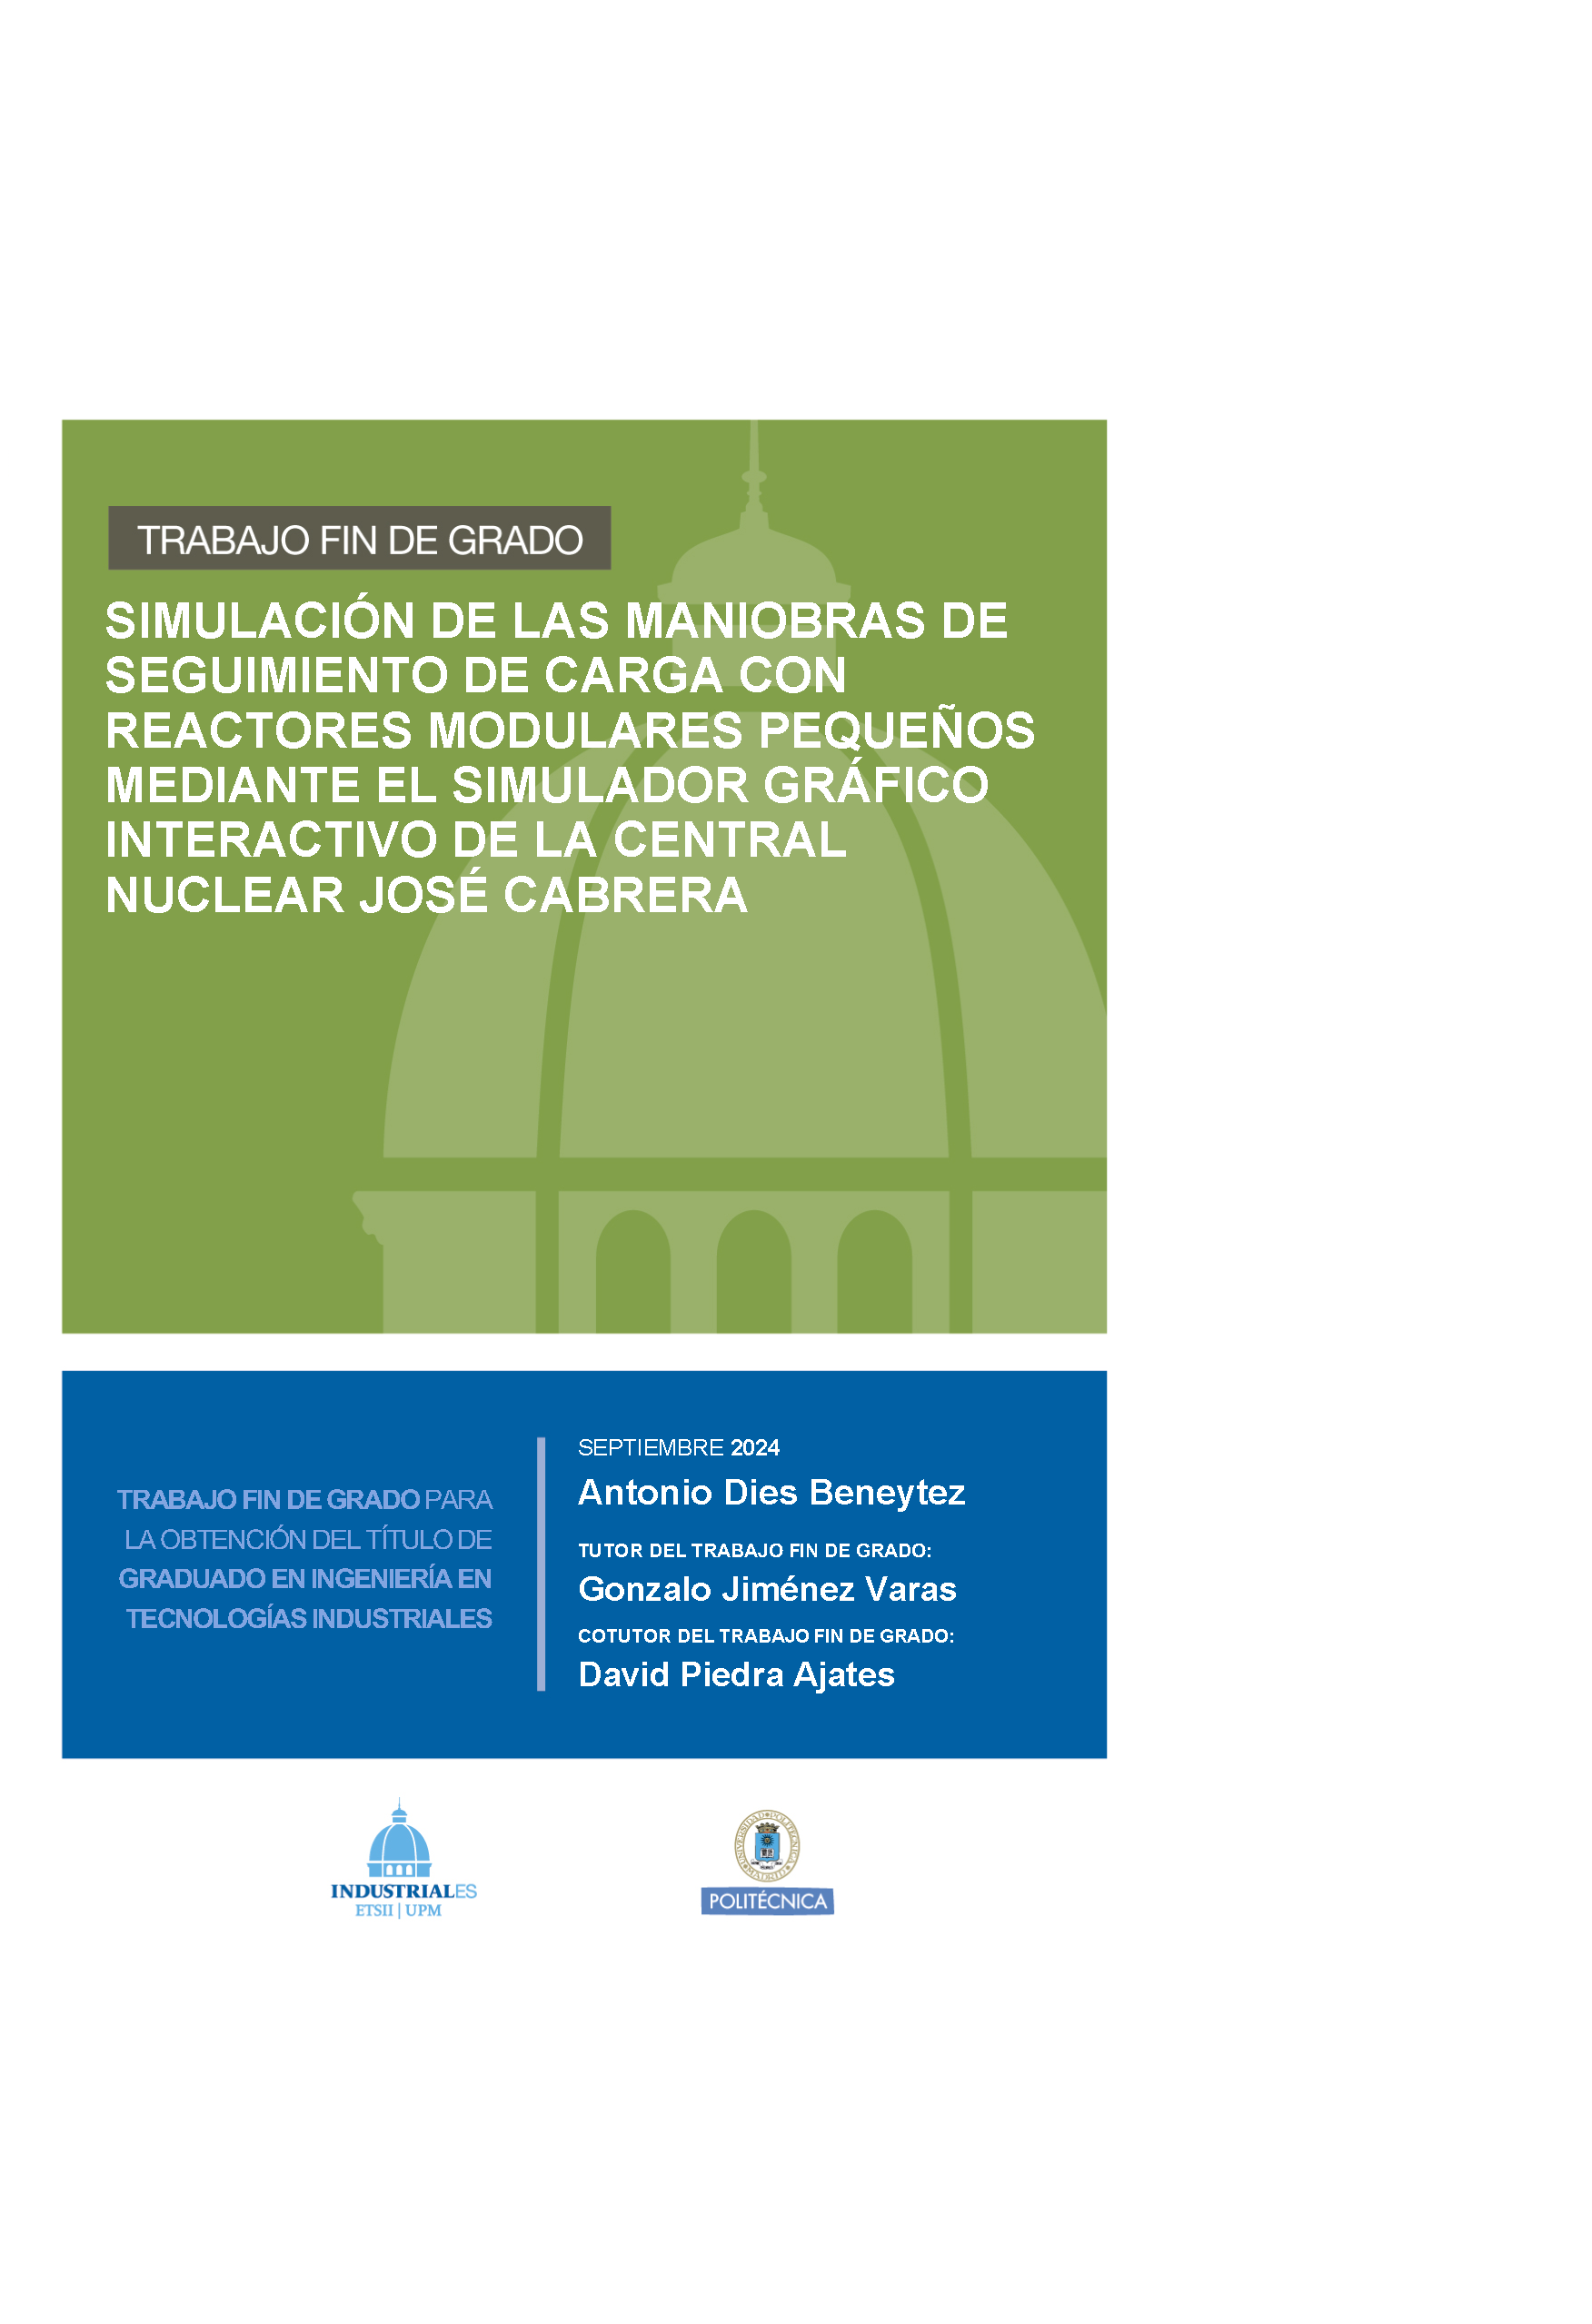
\includepdf{content/Portada_TFG_Antonio_Dies.pdf}  
%%%%%%%%%%%%%%%%%%%%%%%%%%%%%%%%%%%%%%%%%%%%%%%%%%

% Las páginas anteriores al contenido del TFG (previas a la introducción) suelen numerarse en números romanos:
\pagenumbering{roman}


%%%%%%%%%%%%%%%%%% - CITA - %%%%%%%%%%%%%%%%%%%%%
\newpage
\thispagestyle{empty}

\begin{flushright} % Se alinea el texto en el lado derecho de la página.
\vspace*{5cm} % Se añade un espacio vertical de 5cm para situar la cita en ~1/3 de la página.

\textit{“As for the future, your task is not to foresee it, but to enable it.”} 

\medskip % Salto a la línea de tamaño medio (existen \smallskip, \medskip y \bigskip)
- Antoine de Saint-Exupéry

\end{flushright}

\afterpage{\blankpage} % Se añade una página en blanco después de la cita.


%%%%%%%%%%%%% - AGRADECIMIENTOS - %%%%%%%%%%%%%%%%
\newpage
\thispagestyle{plain} % Formato plano (sin encabezado/pie de página pero con número de página):

\section*{AGRADECIMIENTOS} % Se añade un asterisco a \section para que el título no esté numerado.
\addcontentsline{toc}{section}{AGRADECIMIENTOS} % Al utilizar \section* se ha de añadir manualmente el apartado al índice (Table Of Contents, TOC).

Agradezco a \dots

Gracias a \dots

A \dots \ por \dots

\afterpage{\blankpage} % Se añade una página en blanco después de los agradecimientos.

%%%%%%%%%%%%%% - RESUMEN - %%%%%%%%%%%%%
\newpage
\section*{RESUMEN} % Se añade un asterisco a \section para que el título no esté numerado.
\markright{RESUMEN} % Al utilizar \section* se ha de añadir manualmente el título del apartado al encabezado.
\addcontentsline{toc}{section}{RESUMEN} % Al utilizar \section* se ha de añadir manualmente el apartado al índice (Table Of Contents, TOC).

Este resumen deberá tener una extensión máxima de cinco páginas y habrá de constituir una síntesis de los puntos más importantes del proyecto. El resumen debe permitir al lector: 
\begin{itemize}
    \item tener una visión general del trabajo realizado
    \item lograr una comprensión global del proyecto. No importa cuán complejo sea el tema tratado, el resumen debe explicar lo más claramente posible en qué consiste
\end{itemize}

Además, el resumen debe crear interés en el lector para que éste lea todo el contenido del trabajo. Incluir al final Palabras clave y Códigos UNESCO.

\afterpage{\blankpage} % Se añade una página en blanco después del resumen.


%%%%%%%%%%%%%%%%%%% - ÍNDICE - %%%%%%%%%%%%%%%%%%%
\newpage
\renewcommand*\contentsname{ÍNDICE} % Se modifica el nombre por defecto de la "Table Of Contents" (tabla de contenidos, índice) para pasar a llamarla "ÍNDICE".
\tableofcontents % Se genera el índice de contenidos del documento que incorpora todos los títulos de \section, \subsection y \subsubsection (y también \paragraph, ver capítulo 1), así como los títulos añadidos con \addcontentsline (como el resumen ejecutivo, por ejemplo).
\afterpage{\blankpage} % Se añade una página en blanco después del índice.
%%%%%%%%%%%%%%%%%%%%%%%%%%%%%%%%%%%%%%%%%%%%%%%%%%

% Se inicia una nueva página, y se restablece la numeración de las páginas, utilizando esta vez el sistema de numeración estándar (1, 2, 3, 4, ...)
\newpage
\pagenumbering{arabic}

%%%%%%%%%%%%%% - CONTENIDO PRINCIPAL - %%%%%%%%%%%%%%

\section{INTRODUCCIÓN} \label{sec:introduccion}

\subsection{Justificación}

Actualmente, el mundo atraviesa una crisis energética global desencadenada en el año 2021 principalmente por la recuperación económica tras la pandemia y agravada tras la invasión rusa de Ucrania en febrero de 2022. El precio del gas natural alcanzó máximos históricos, aumentando consecuentemente en muchos casos el coste de la electricidad en general. Familias, empresas e industrias se han visto gravemente afectadas, llevando a diversos países en camino de una fuerte recesión económica. Consecuentemente, la reducción de los costes energéticos se convierte en una de las principales prioridades de empresas y ciudadanos, y la independencia energética, la
garantía de suministro y la lucha contra el cambio climático adquieren una gran importancia en el debate público de gran cantidad de países (\cite{crisis_energetica_iea}). 

Frente a esta situación, la energía nuclear está tomando cada vez más relevancia en muchos países, considerándose un factor clave para conseguir los grandes desafíos políticos, económicos y climáticos  a los que se enfrenta la sociedad actual en un escenario tan complicado. Numerosos países han optado por ampliar su parque nuclear existente, muchos han decidido alargar la vida de sus reactores nucleares actualmente en operación y algunos han comenzado a construir sus primeras centrales nucleares. 

\begin{table}[h]
    \resizebox{\textwidth}{!}{%
    \begin{tabular}{|cc|cc|cc|}
    \hline
    \rowcolor[HTML]{ECF4FF} 
    \multicolumn{2}{|l|}{\cellcolor[HTML]{ECF4FF}\textbf{Generación de electricidad nuclear}} &
      \multicolumn{2}{l|}{\cellcolor[HTML]{ECF4FF}\textbf{Reactores en operación}\tablefootnote{\textbf{En operación:} Conectados a la red.}} &
      \multicolumn{2}{l|}{\cellcolor[HTML]{ECF4FF}\textbf{Reactores en construcción}\tablefootnote{\textbf{En construcción:} primer hormigón vertido para el reactor.}} \\ \hline
    \rowcolor[HTML]{FFFFFF} 
    \multicolumn{1}{|c|}{\cellcolor[HTML]{FFFFFF}\textbf{9,8}} &
      2.808 TWh &
      \multicolumn{1}{c|}{\cellcolor[HTML]{FFFFFF}\textbf{436}} &
      392.114 MWe &
      \multicolumn{1}{c|}{\cellcolor[HTML]{FFFFFF}{\color[HTML]{000000} \textbf{62}}} &
      {\color[HTML]{000000} 69.279 MWe} \\ \hline
    \rowcolor[HTML]{ECF4FF} 
    \multicolumn{2}{|c|}{\cellcolor[HTML]{ECF4FF}\textbf{Reactores planificados}\tablefootnote{\textbf{Planificados:} Aprobaciones, financiamiento o compromiso en vigor. Se espera que estén en funcionamiento en los próximos 15 años.}} &
      \multicolumn{2}{c|}{\cellcolor[HTML]{ECF4FF}\textbf{Reactores propuestos}\tablefootnote{\textbf{Propuestos:} Programa específico o propuestas de sitio; tiempo muy incierto.}} &
      \multicolumn{2}{c|}{\cellcolor[HTML]{ECF4FF}\textbf{OLP aprobada}\tablefootnote{\textbf{\acrfull{olp} aprobada:} Autorización a operar más allá de los 40 años. En Estados Unidos, la mayoría de reactores tiene licencia para operar a 60 años y 6 tienen permiso para operar hasta los 80.}} \\ \hline
    \multicolumn{1}{|c|}{\cellcolor[HTML]{FFFFFF}\textbf{110}} &
      \cellcolor[HTML]{FFFFFF}112.877 MWe &
      \multicolumn{1}{c|}{\cellcolor[HTML]{FFFFFF}\textbf{333}} &
      \cellcolor[HTML]{FFFFFF}366.652 MWe &
      \multicolumn{2}{c|}{\textbf{191}} \\ \hline
    \end{tabular}%
    }
    \caption{Resumen de la situación actual de la energía nuclear en el mundo (\cite{world_nuclear_power_reactors}).}
    \label{tab:situacion_nuclear_mundial}
    \end{table}

    \begin{wrapfigure}{r}{0.52\textwidth}
      \vspace{-0.5cm}
      \centering
      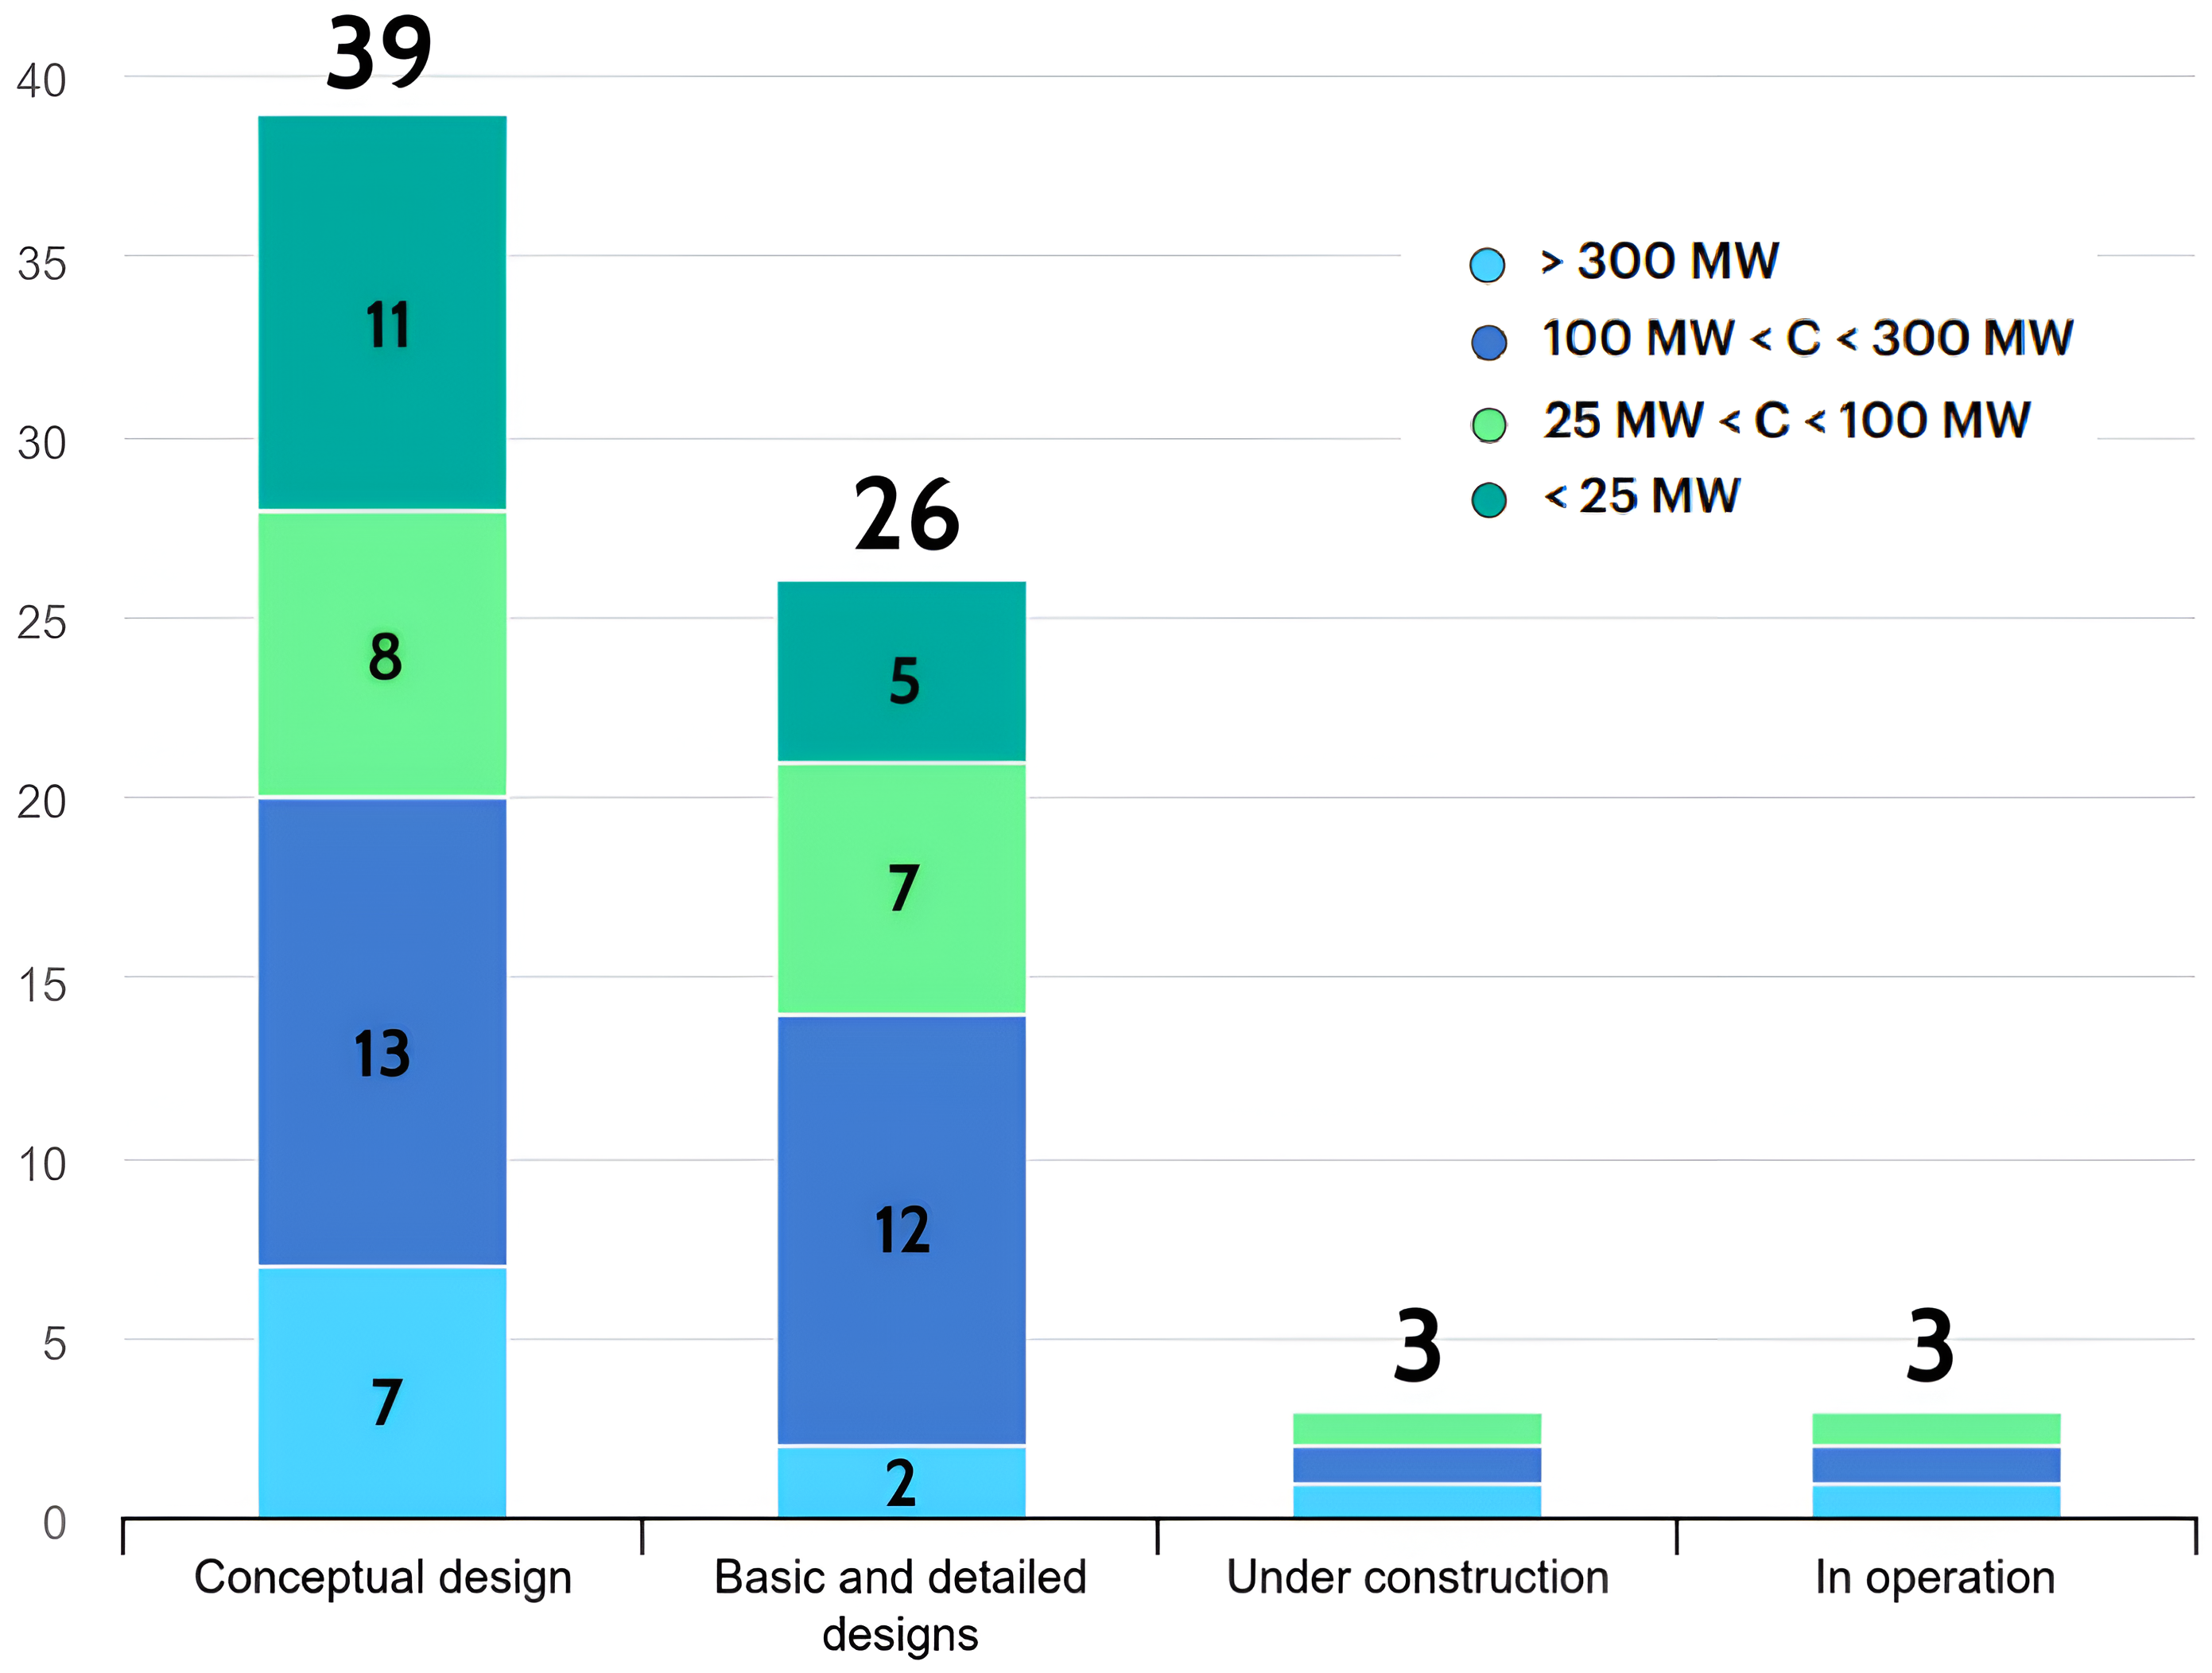
\includegraphics[width=0.52\textwidth]{content/figures/global_smr_projects2.png}
      \caption{\acrshortpl{smr} en el mundo (\cite{iea_global_smr_projects}).}
      \label{fig:global_smr_projects}
      \vspace{-1cm}
    \end{wrapfigure}

    En este contexto, se ha incrementado muy considerablemente el interés por los reactores modulares pequeños, ampliamente conocidos como \emph{\acrfullpl{smr}}. Se trata de una tecnología avanzada de menor escala que la convencional que ofrece grandes ventajas en lo que a coste, tiempo de construcción, seguridad y versatilidad se refiere. Por consiguiente, múltiples instituciones públicas y privadas están participando activamente en los esfuerzos encaminados a hacer prosperar esta tecnología, existiendo más de 80 diseños de \acrshortpl{smr} comerciales que se están desarrollando en todo el mundo (\cite{smr_oiea}).




    
\newpage 

Este creciente empuje de la industria nuclear está contribuyendo a un aumento de profesionales especializados en este sector y, paralelamente, a una creciente necesidad de futuros profesionales nucleares. En este contexto y frente a los grandes avances tecnológicos desarrollados actualmente, cobran una especial importancia los \textbf{simuladores} empleados tanto en el ámbito del análisis numérico como en la formación de operadores, técnicos e ingenieros nucleares. Existen múltiples simuladores virtuales y físicos desarrollados por diversas instituciones y empresas que permiten enfrentarse a las condiciones de operación, maniobras y accidentes que pueden suceder en una central nuclear. La Escuela Técnica Superior de Ingenieros Industriales de Madrid (ETSII - UPM) tiene a su disposición el \acrfull{sgiz}, con el cual se trabajará en el presente proyecto para profundizar en el estudio de la operación de las centrales nucleares y, en concreto, en la operación de un \acrshort{smr}, debido a las grandes similitudes que el simulador en cuestión presenta con respecto a esta innovadora tecnología.

\subsection{Objetivos}

El principal objetivo de este trabajo fin de grado es \textbf{simular maniobras de seguimiento de carga de una central nuclear muy similar a un \acrshort{smr}} mediante el \acrshort{sgiz} de la Escuela. Este tipo de maniobras es una de las aplicaciones fundamentales para las que se concibe el diseño de los \acrshortpl{smr} y presentan un gran interés actualmente. Para ello, y como segundo objetivo fundamental, se pretende \textbf{conocer en profundidad el funcionamiento de un \acrshort{smr}; sus sistemas de seguridad, protección y control, y su modo de operación}.

Asimismo, existen paralelamente diversos objetivos secundarios. En primer lugar, familiarizarse con el tipo de software empleado en los simuladores del ámbito nuclear. En segundo lugar, conocer el estado del arte, las características, las grandes ventajas y los desafíos de la tecnología de los \acrshortpl{smr}. Por último, implementar las simulaciones realizadas al programa de prácticas de la asignatura de Tecnologías Avanzadas en Reactores Nucleares del Máster en Ciencia y Tecnología Nuclear impartido en la ETSII.

\subsection{Metodología}

El desarrollo de este proyecto parte de una adquisición completa de diversos conceptos teóricos que permitirán posteriormente focalizarse en la realización de simulaciones prácticas. Al mismo tiempo, estas simulaciones complementarán y consolidarán los conocimientos previos adquiridos y posibilitarán un aprendizaje en profundidad. De esta manera, el trabajo se fundamenta, en tres grandes bloques:

\begin{itemize}
  \item \textbf{Los \acrlongpl{smr}:} Comenzando por los orígenes de esta tecnología, posteriormente se analizan detalladamente las ventajas que presenta frente a los reactores de gran escala y se clasifican los distintos tipos de pequeños reactores modulares existentes. Por último, se analiza un \acrshort{smr} en concreto ---el AP300--- por su similitud con el reactor del simulador con el que se trabaja ---el \acrshort{sgiz}---.
  \item \textbf{Los simuladores:} En primer lugar, se clasifican los distintos tipos de simuladores existentes en función de los objetivos, las ventajas y las funcionalidades que presentan. En segundo lugar, se analizan casos concretos de simuladores de \acrshortpl{smr} para conocer el estado del arte de este tipo de simulación. Seguidamente, se detallan las ventajas del empleo de simuladores para fines formativos y didácticos. Por último, se estudia la Central Nuclear de Zorita, a la cual pertenece el \acrshort{sgiz}, comparándola con el AP300 para ver su parecido con un \acrshort{smr}. Además, se finaliza este estudio con una descripción de las características y modos de operación del \acrshort{sgiz}.
  \item \textbf{Las simulaciones:} Como el proyecto se centra en el análisis de las capacidades de seguimiento de carga de los \acrshortpl{smr}, se comienza este apartado práctico con un estudio de este tipo de maniobras de variación de potencia en función de distintas necesidades. Seguidamente, se realizan múltiples simulaciones que, tras ser debidamente analizadas, permiten comprender en profundidad, no solo el seguimiento de carga, sino también el funcionamiento y los  sistemas más importantes de una central nuclear. En este bloque se incluye la implementación de una de las simulaciones como práctica académica.
\end{itemize}
\newpage
\section{\emph{SMALL MODULAR REACTORS (SMRs)}} \label{small_modular_reactors}

Los reactores modulares pequeños, más conocidos como \acrfullpl{smr}, son \textbf{reactores nucleares avanzados que producen entre 10 y 300 MWe por módulo} (\cite{nea_smrs_2021}). Aunque se trata de una potencia considerablemente menor a la de los reactores nucleares convencionales de alta potencia ---que suele ser de más de 1.000 MWe---, es precisamente esta característica la que los hace muy atractivos, dadas las múltiples ventajas que esto proporciona en cuanto a versatilidad y variedad de aplicaciones.

Actualmente, hay un creciente interés por esta innovadora tecnología. Durante la \emph{Conferencia Internacional sobre el Cambio Climático y el Papel de la Energía Nuclear} celebrada en septiembre de 2019, muchos Estados Miembros consideraron a los \acrshortpl{smr} como ``una opción nuclear potencialmente viable para contribuir a mitigar el cambio climático'' (\cite{oiea_informe_2019}). A raíz de esta conferencia, en abril de 2021, el \acrfull{oiea} creó la \emph{Plataforma sobre Reactores Modulares Pequeños y sus Aplicaciones (Plataforma SMR)}, un mecanismo que coordina las actividades del \acrshort{oiea} en este campo y proporciona un punto de encuentro común para los Estados Miembros y otras partes interesadas. Por último, cabe destacar que la Comisión Europea creó el pasado 6 de febrero de 2024 una alianza con el objetivo de facilitar y acelerar el desarrollo y el despliegue de los primeros proyectos de \acrshortpl{smr} en Europa a principios de la década de 2030: la \emph{Alianza Europea Industrial en SMRs}. Todo esto refleja una apuesta creciente por los pequeños reactores modulares que debe ir acompañada por un fuerte impulso en el \acrshort{idi} en este ámbito.

\subsection{Breve recorrido histórico: Orígenes y desarrollo}

El origen de los \acrshortpl{smr} es militar y se remonta a los años 50, cuando se diseñaron por primera vez los pequeños reactores que se emplearon para la propulsión naval de submarinos nucleares, portaviones y rompehielos. Con la elaboración del primer subarino nuclear, el \emph{Nautilus}, diseñado por la armada estadounidense y puesto en marcha en enero de 1955, se puso de manifiesto las importantes ventajas que esta tecnología ofrecía a los grandes navíos militares: posibilidad de inmersión por tiempo ilimitado ---en el caso de los submarinos--- al no requerir oxígeno para su funcionamiento, alto nivel de disponibilidad y de independencia de abastecimiento de combustible, elevada versatilidad y mayores velocidades de desplazamiento (\cite{propulsion_naval_nuclear}).

\begin{figure}[h]
    \centering
    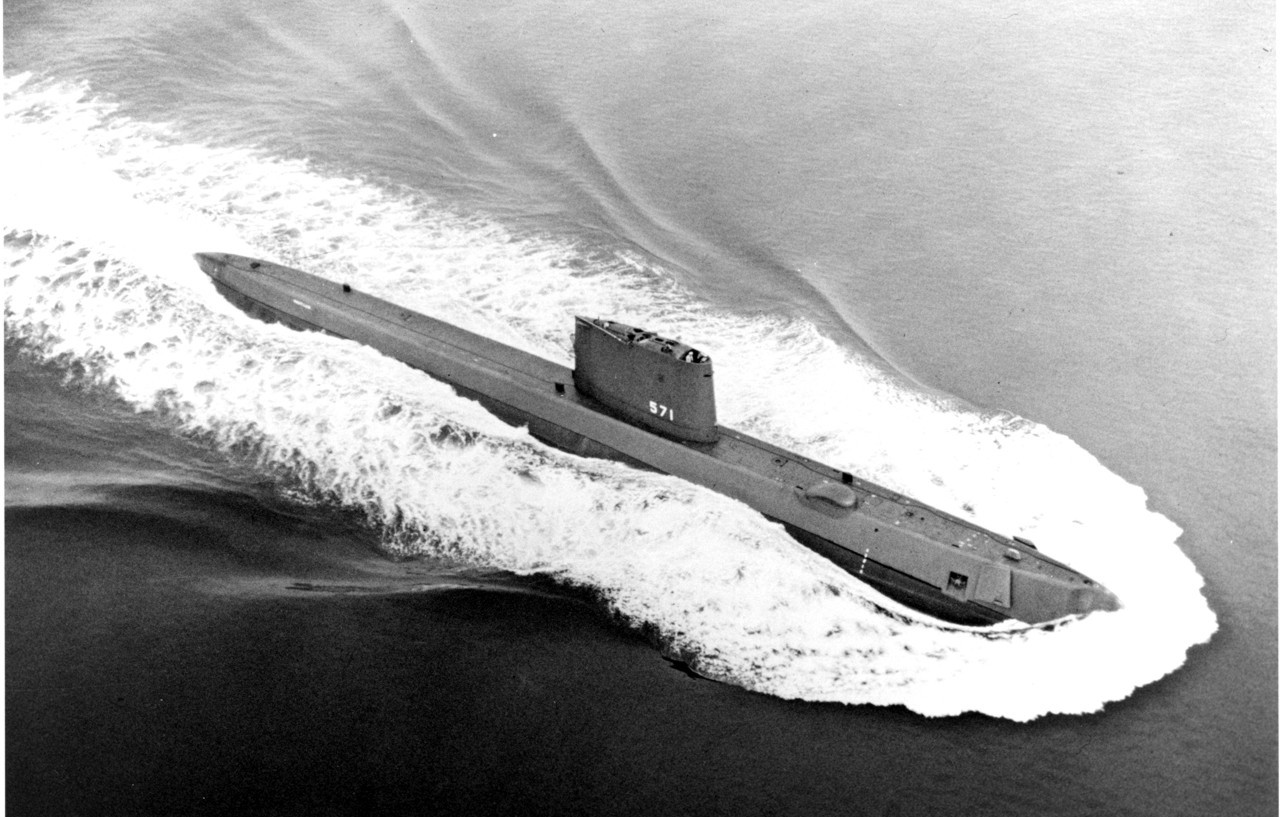
\includegraphics[width=0.55\textwidth]{content/figures/nautilus.jpg}
    \caption{\emph{USS Nautilus (SSN-571)} en alta mar con su reactor S2W de 10 MW de Westinghouse (\cite{poder_naval}).}
    \label{fig:nautilus}
\end{figure}

No fue, sin embargo, hasta más adelante cuando empezaron a desarrollarse los pequeños reactores nucleares comerciales para uso civil. El primer prototipo fue diseñado en 2007 por un equipo de científicos estadounidenses de la \emph{Oregon State University (OSU)} y se le llamó \emph{Multi-Application Small Light Water Reactor (MASLWR)}. Con una potencia de 45 MWe, el MASLWR, fue el prototipo con el que empezó a trabajar la empresa \emph{NuScale Power}, la cual consiguió lanzar en 2022 al mercado estadounidense el primer \acrshort{smr} apto para operar.

Hoy en día \textbf{existen en todo el mundo más de 80 diseños y conceptos de \acrshort{smr}} en diversas etapas de desarrollo, cuatro de los cuales se encuentran en etapas avanzadas de construcción en Argentina, China y Rusia.

\subsection{Características generales}

Los diseños de \acrshortpl{smr} están progresando rápidamente, partiendo del objetivo de integrar sistemas para conseguir modulizar los reactores al mismo tiempo que se introducen mejoras significativas para el funcionamiento eficaz y seguro de los mismos. De esta manera, se están desarrollando prototipos con muy buenas prestaciones en lo que a seguridad, flexibilidad, costes, gestión de residuos y variedad de aplicaciones se refiere.

\subsubsection{Seguridad} \label{seguridad}

Debido a la experiencia de más de 60 años de operación de las centrales nucleares, se han llevado a cabo gradualmente grandes mejoras de seguridad y control de las mismas. Los reactores nucleares avanzados que se están desarrollando en los últimos años, incluidos los \acrshortpl{smr}, incorporan estos avances tecnológicos. Entre las múltiples mejoras incorporadas, cabe destacar el empleo de innovadores \textbf{sistemas de seguridad pasiva}. Los sistemas pasivos son aquellos que no requieren de la acción de un operador o de realimentación electrónica para funcionar, sino que su actuación se asegura por principios físicos independientes de energía externa. Son, por tanto, especialmente útiles en casos de emergencia en los que, aunque se perdiera el suministro eléctrico de la central, los sistemas de seguridad deberían funcionar sin ningún problema (\cite{glosario_seguridad_oiea}). Algunos ejemplos de este tipo de sistemas son los r\gls{ecombinadores pasivos} autocatalíticos\footnote{Eliminan los posibles gases combustibles generados dentro de la contención en accidentes severos mediante la recombinación o combustión de una manera gradual, minimizando así el riesgo de una explosión de hidrógeno.}, el \acrfull{svfc}\footnote{Posibilita la despresurización controlada del Edificio de Contención en caso de fusión del núcleo y la reducción de la cantidad de material radiactivo que podría ser liberado al exterior.} o el sistema de sellado pasivo de las bombas del circuito primario\footnote{Permite reducir significativamente o, incluso, eliminar la fuga de refrigerante a través de los sellos sin requerir operación manual. Se activan por temperatura y bloquean automáticamente
el paso de agua.}. Todos estos nuevos sistemas se han ido implementando en las centrales nucleares actualmente en operación y se han incorporado, junto con muchos otros avances, en los diseños de los reactores avanzados.

En el caso de los \acrshortpl{smr}, la mayor dependencia de los mecanismos de seguridad pasiva, al reducir la necesidad de sistemas activos ---como las bombas de refrigeración del reactor---, simplifica las evaluaciones de seguridad y reduce las posibilidades de fallo de la instalación. La menor potencia de salida y la mayor relación superficie-volumen ofrecida por núcleos más pequeños aumentan la eficiencia de los sistemas de seguridad pasiva tanto para condiciones de operación normales como para transitorios indeseados. Por ejemplo, muchos diseños de tipo \acrshortpl{lwr} disponen de grandes depósitos de agua para enfriar pasivamente los sistemas de reactor incluso en circunstancias extremas (por ejemplo, en caso de pérdida de suministro eléctrico exterior). Una mayor dependencia de los sistemas de enfriamiento pasivo permite \textbf{diseños más simplificados y una operación y mantenimiento más eficientes}. 

Por otro lado, su \textbf{diseño integral} incorpora todos los componentes del \gls{sistema de suministro de vapor nuclear} (del inglés, \acrshort{nsss})\footnote{Incluye los principales sistemas y componentes de una central nuclear: todo el sistema del refrigerante del reactor (el circuito primario), los sistemas fluidos auxiliares y los principales sistemas eléctricos, de instrumentación y control requeridos para la operación de la planta.} en un solo recipiente. Consecuentemente, la mayor relación superfície-volumen de estos reactores mejora la disipación del calor residual. Esto implica que la cantidad de refrigerante contenido en la vasija del reactor es considerablemente mayor que en las configuraciones tradicionales de bucle externo, lo cual aumenta la capacidad calorífica\footnote{Cantidad de energía necesaria para aumentar la temperatura de un sistema en una unidad de temperatura.} y la inercia térmica\footnote{Capacidad que tiene un sistema de almacenar calor. Es directamente proporcional a la capacidad calorífica, por lo que a mayor inercia térmica, mayor cantidad de energía se requiere para elevar la temperatura de un cuerpo.} del sistema. Además, para la extracción del calor residual se han desarrollado nuevas metodologías, como apoyar la refrigeración convencional con la convección natural de aire.

\begin{figure}[h]
  \centering
  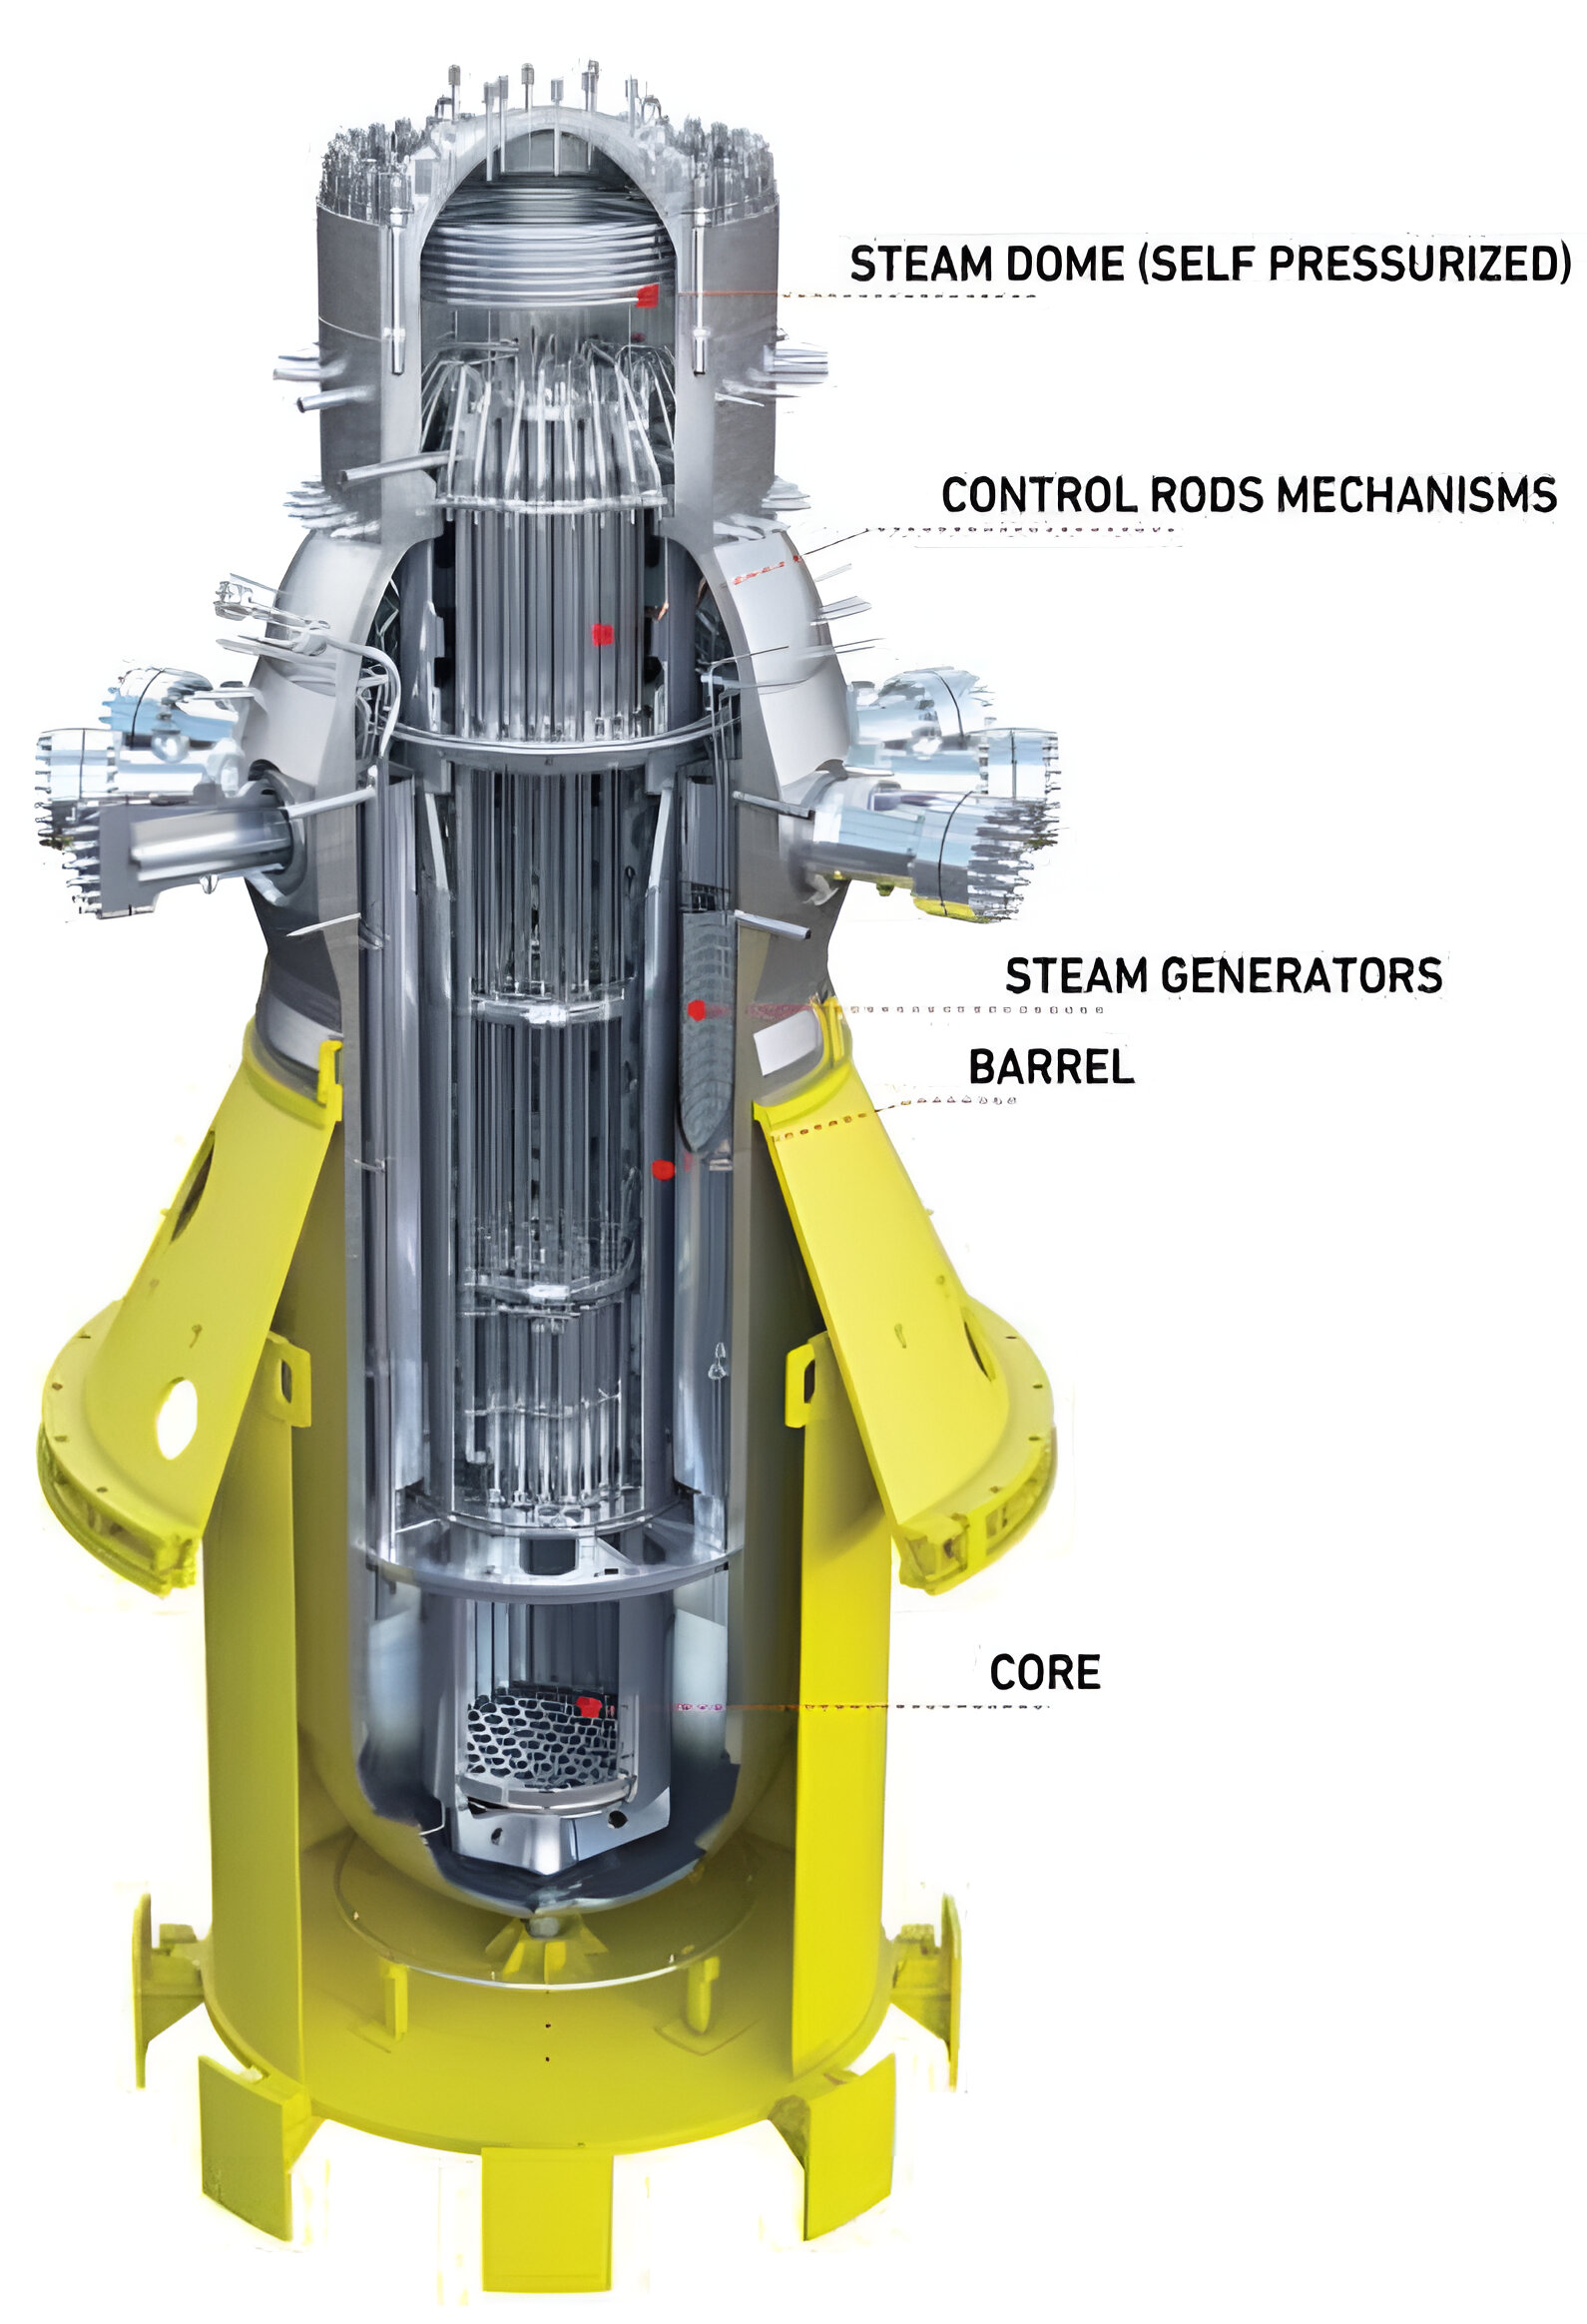
\includegraphics[width=0.62\textwidth]{content/figures/carem.jpeg}
  \caption{Vasija del reactor CAREM (ver tabla \ref{tab:smrs_agua_tierra}) que alberga de forma integral los componentes del \acrshort{nsss}: el núcleo, los generadores de vapor, el refrigerante primario, etc. junto con otros elementos fundamentales, como las barras de control (\cite{iaea_smr_booklet_2022}).}
  \label{fig:carem}
\end{figure}

La compacta configuración de los \acrshortpl{smr} \textbf{reduce la probabilidad de accidentes y la gravedad de los mismos}. Por ejemplo, un diseño más compacto reduce considerablemente el número de penetraciones en la vasija de reactor para la instalación de tubos, lo cual se traduce en una disminución del número de puntos con probabilidad de fuga, haciendo así más resistente al reactor frente a un accidente de pérdida de refrigerante (del inglés, \acrshort{loca}). Otro ejemplo es que la integración de las barras de control dentro de la vasija del reactor elimina el riesgo de accidentes por eyección de las mismas, suceso que puede ocurrir en un reactor convencional y que provoca un súbito incremento de reactividad y, por tanto, un aumento incontrolado de la potencia del reactor. Cabe mencionar, por último, que al trabajar con mayor inercia térmica y menor densidad de potencia\footnote{Cantidad de potencia generada por unidad de volumen. En los \acrshortpl{smr}, al ser mucho menor la potencia generada, la potencia densidad específica es baja.}, la respuesta frente a transitorios de temperatura es más lenta, lo cual aumenta los márgenes de seguridad y ralentiza el posible descontrol del reactor en situaciones adversas.

Además, la reducción del inventario del núcleo del reactor hace que se requiera \textbf{menos blindaje} para la protección del mismo y que las dosis de exposición de los trabajadores sean menores. Tal y como se ha comentado en el párrafo anterior, el hecho de tener un núcleo más pequeño reduce la probabilidad de accidente e implica menor energía en la posible expulsión de emisiones radiactivas. De esta manera, \textbf{se reduce la extensión necesaria de las zonas de planificación de emergencia (\acrshortpl{epz})}\footnote{Zonas que rodean a la central nuclear que se proveen, en base al plan de emergencia correspondiente, de las necesarias medidas de protección de cara a un posible accidente}. Esto último implica que estas plantas podrían ubicarse más cerca de los consumidores finales, ofreciendo un servicio más directo y reduciendo los problemas derivados del transporte de electricidad a grandes distancias.

Por último, las características de los \acrshortpl{smr} hacen posible su \textbf{ubicación subterránea}, que proporciona una mayor protección frente a posibles peligros naturales ---terremotos, inundaciones, huracanes, etc.--- o provocados por el ser humano ---como podría ser el impacto de un avión---. Múltiples diseños desarrollados en los últimos años, como el que se muestra en la figura \ref{fig:ultra_safe_nuclear_mmr}, están optando por ubicar de esta manera los principales componentes de la planta (\cite{nea_smrs_2021}).

\begin{figure}[h]
  \centering
  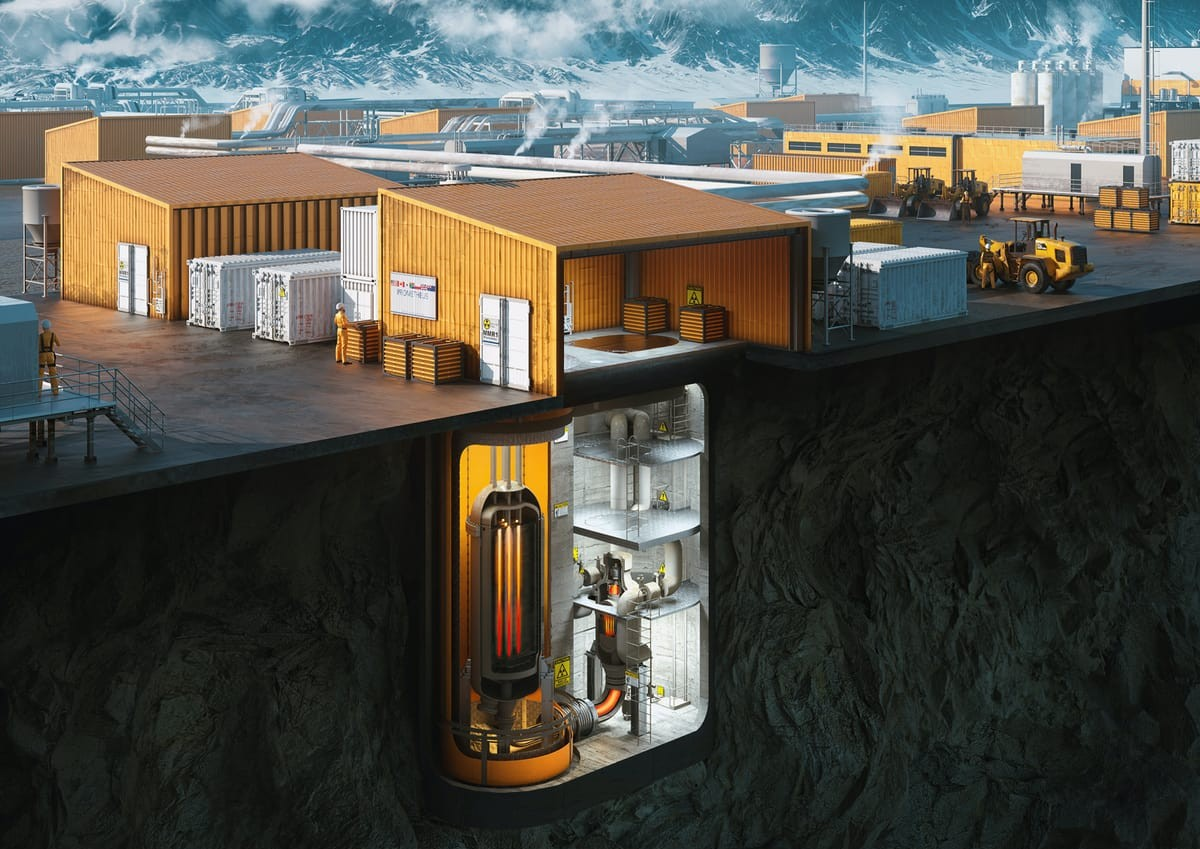
\includegraphics[width=0.65\textwidth]{content/figures/ultra_safe_nuclear_mmr.jpg}
  \caption{\emph{\acrshort{mmr} Energy System} (ver tabla \ref{tab:mmrs}) de entre 3,5 y 15 MWe de potencia, diseñado por la \emph{Ultra Safe Nuclear Corporation} (\cite{ultra_safe_nuclear_corporation}).}
  \label{fig:ultra_safe_nuclear_mmr}
\end{figure}

\subsubsection{Modularidad} \label{modularidad}

La \emph{modularización} es una forma de simplificar la construcción de un equipo mediante su división en módulos más pequeños que pueden construirse en fábrica, para ser posteriormente transportados a su destino y finalmente ensamblados allí mismo. En el ámbito nuclear, aunque esta técnica ya ha sido empleada para la construcción de algunas centrales nucleares de gran escala, los \acrlongpl{smr} aprovechan aún más las \textbf{ventajas} que confiere este tipo de construcción en cuanto a eficiencia, coste y seguridad:

\begin{itemize}
  \item El hecho de realizar la fabricación o el pre-ensamblaje de los módulos en una fábrica preparada para ello ---fuera del sitio de construcción--- con una metodología en serie estandarizada, aumenta la productividad laboral, asegura un mejor control de calidad de todos los componentes y reduce los riesgos derivados de la gestión del proyecto, al ser más predecible la evolución material y temporal del mismo.
  \item El pequeño tamaño de los módulos ---al tratarse de reactores de escala reducida--- permite una buena transportabilidad y maniobrabilidad de los mismos. Varios desarrolladores de \acrshort{smr} han estudiado y garantizado la posibilidad de transportar el módulo completo del sistema de suministro de vapor nuclear (\acrshort{nsss}) usando camiones convencionales, barcos o por ferrocarril.
  \item Actualmente, la modularización y producción en fábrica ya aplica aproximadamente al 30\% de la construcción de los reactores nucleares. Sin embargo, se prevee una capacidad de modularización de hasta el 60 - 80\% en el proceso de construcción de los pequeños reactores modulares (\cite{nea_unlocking_2020}).
  \item La manufactura en fábrica permite emplear técnicas avanzadas de fabricación ---como, por ejemplo, la soldadura láser o la fabricación aditiva--- que serían muy difíciles de implementar si se tratase de fabricación \emph{in situ}. Este tipo de técnicas avanzadas reduce el número de soldaduras necesarias y elimina las costosas inspecciones de calidad en servicio. Asimismo, las tecnologías punteras de digitalización y automatización de las cadenas de producción implican una disminución adicional del coste y del tiempo de entrega de los componentes.
  \item Finalmente, estas reducciones en la duración de la construcción de los \acrshortpl{smr} implica una mayor velocidad para llegar al mercado, ya que hace más predecibles los tiempos y elimina la incertidumbre temporal que a veces se da en los proyectos de las grandes centrales nucleares.
\end{itemize}

Sin embargo, la construcción modular presenta también ciertos \textbf{inconvenientes}:

\begin{itemize}
  \item El diseño adecuado de los módulos que compondrán la instalación es un verdadero desafío tecnológico e ingenieril, lo cual supone mayores esfuerzos en la concepción constructiva de los mismos.
  \item Los materiales y componentes de los distintos módulos deben ser adquiridos antes de comenzar la construcción, lo que supone un aumento de la inversión inicial.
\end{itemize}

\newpage
\subsubsection{Combustible y gestión de residuos} \label{combustible}

En lo que se refiere al \emph{front end} o fase pre-reactor del ciclo de combustible de los \acrlongpl{smr} de tipo \acrshort{lwr}, se prevee un desarrollo compatible con la tecnlogoía empleada en los ciclos de combustible actuales, con enriquecimientos  por debajo del 5\%. Además, se esperan ciclos de operación más largos: de 36 a 40 meses, frente a los 18 - 24 meses de los \acrshortpl{lwr} existentes. Esto último se debe a que el tamaño del núcleo es más reducido y estos reactores avanzados se diseñan para aprovechar más eficientemente el combustible o con capacidad de emplear nuevos combustibles avanzados con mayor \gls{grado de quemado}\footnote{El grado de quemado es la energía extraída por unidad de masa de combustible presente en el reactor. En general, al trabajar a más bajas potencias, el grado de quemado de los \acrshortpl{smr} es inferior que el de los reactores de gran escala. Sin embargo, los diseños más recientes buscan grados de quemado muy elevados para aumentar la eficiencia, los períodos entre recargas y la seguridad.}. Esto se traduce en una disminución de costes de capital y operativos, y en menores riesgos por la menor cantidad de combustible con la que se trabaja (\cite{overview_smrs}).

En el caso de los microrreactores ---los de \gls{tubos de calor}\footnote{Los microrreactores refrigerados con tubos de calor ---\acrfull{hpr}--- eliminan pasivamente el calor del núcleo  utilizando tubos de calor. Estos tubos son dispositivos pasivos de transferencia de calor que usan la fuerza capilar de su estructura interna y juegan con los cambios de fase. El tubo de calor contiene un fluido de trabajo que transfiere calor al evaporarse en la sección evaporadora y se condensa en la sección condensadora. Se trata de reactores con un diseño compacto, de fácil transporte y con una elevada estabilidad del sistema.}, principalmente--- y los \acrshortpl{smr} de \acrshort{genIV}, se calculan períodos de operación entre recargas de hasta 20 años. De hecho, los reactores que emplean \textbf{\gls{combustible} \acrshort{triso}}\footnote{Combustible tri-isotrópico empleado en reactores de alta temperatura formado por carburo de uranio revestido con varias capas de carbón pirolítico y $SiO_2$ para retener los productos de fisión a elevadas temperaturas.} o los refrigerados por sales fundidas se diseñan para poder realizar las recargas sin dejar de funcionar.

Paralelamente, varios diseños de \acrshort{smr} están considerando el empleo de \textbf{uranio de alto ensayo y bajo enriquecimiento} (entre el 5 - 19,75\%), el \acrfull{haleu}, el cual ofrece muy buenas prestaciones en lo que se refiere a un elevado grado de quemado, menor tamaño de núcleo requerido, períodos de operación más largos y posibilidad de aprovechamiento del uranio empobrecido de los elementos de combustible irradiados. Combustibles con tan elevado enriquecimiento son necesarios para los reactores nucleares de espectro neutrónico rápido o para reactores de propulsión naval, que de momento emplean uranio altamente enriquecido (del inglés, \acrshort{heu}), cuyas existencias se prevee que podrían agotarse para la década del 2030. Es por esto que, pese a que anteriormente el uso del \acrshort{haleu} se limitaba a reactores de investigación y a la producción de radioisótopos médicos, el organismo regulador en materia nuclear de EEUU, la \acrfull{nrc}, ha autorizado recientemente el inicio de la producción de este tipo de combustible, sometiéndolo al riguroso control y las múltiples inspecciones que conlleva trabajar comercialmente con enriquecimientos elevados.  Cabe mencionar que, para que en el futuro se dé un suministro estable de este combustible, se requieren mejoras en la infraestructura actual del ciclo de combustible convencional, desarrollando particularmente las instalaciones de enriquecimiento, reconversión y fabricación del combustible. Asimismo, habría que asegurar un transporte adecuado del combustible y una correcta gestión de los residuos radiactivos de alta actividad generados (\cite{nrc_haleu}). 

Por otro lado, muchas empresas desarrolladoras no descartan la posibilidad de emplear \textbf{óxido mixto de uranio (del inglés, \acrshort{mox})} en sus reactores. Se trata de un combustible compuesto por una mezcla de óxido de uranio natural, uranio empobrecido y óxido de plutonio ---la proporción de plutonio varía del 3 al 10\%--- que tiene grandes ventajas:

\begin{itemize}
  \item Su comportamiento es análogo ---con un grado de quemado similar--- al del combustible convencional de bajo enriquecimiento, empleado en la mayoría de reactores de tipo \acrshort{lwr}.
  \item Puede elaborarse a partir del $U^{235}$ ---remanente--- y $Pu^{239}$ ---generado a partir de las capturas neutrónicas y posteriores desintegraciones del $U^{238}$--- presentes en los elementos de combustible irradiados, llevando a cabo así el \textbf{reciclado del combustible "gastado"}, el cual conserva más de un 90\% de su capacidad energética inicial. 
  \item El plutonio necesario también puede obtenerse del armamento militar desactivado, contribuyendo así a la \gls{no prolifera}ción nuclear\footnote{La no ploriferación nuclear consiste en un programa promovido principalmente por la \acrshort{onu} para la cooperación entre países con el fin de emplear la energía nuclear con fines pacíficos e impulsar el desarme nuclear.} (\cite{wna_mox}).
\end{itemize}

Por último, son pocos los \acrshortpl{smr} de \acrshort{genIV} con reactores de espectro neutrónico rápido que estén considerando actualmente emplear plutonio como combustible. Cabe destacar el Reactor de Sal Estable (del inglés, \acrshort{ssr}) de la empresa Moltex, que emplea el $Pu^{240}$ remanente en el combustible irradiado de otras centrales nucleares (\cite{nea_smrs_2021}).

A continuación se expone una tabla comparativa de los combustibles empleados en distintos tipos de reactores nucleares ---tanto de gran como de pequeña escala---, en la cual se ponen de manifiesto las consideraciones que se han explicado en este apartado:

\begin{table}[h]
  \centering
  \resizebox{\textwidth}{!}{%
  \begin{tabular}{|
    >{\columncolor[HTML]{FFCCC9}}c ccccc|}
    \hline
    \multicolumn{1}{|c|}{\cellcolor[HTML]{ECF4FF}\textbf{Diseño}} &
      \multicolumn{1}{c|}{\cellcolor[HTML]{ECF4FF}\textbf{Combustible}} &
      \multicolumn{1}{c|}{\cellcolor[HTML]{ECF4FF}\textbf{\begin{tabular}[c]{@{}c@{}}Enriquecimiento\\ (\%)\end{tabular}}} &
      \multicolumn{1}{c|}{\cellcolor[HTML]{ECF4FF}\textbf{\begin{tabular}[c]{@{}c@{}}Eficiencia\\ térmica (\%)\end{tabular}}} &
      \multicolumn{1}{c|}{\cellcolor[HTML]{ECF4FF}\textbf{\begin{tabular}[c]{@{}c@{}}Grado de \\ quemado\\ (GWd/tU)\end{tabular}}} &
      \cellcolor[HTML]{ECF4FF}\textbf{\begin{tabular}[c]{@{}c@{}}Período entre\\ recargas (meses)\end{tabular}} \\ \hline
    \multicolumn{6}{|c|}{\cellcolor[HTML]{FFCE93}\textbf{Reactor de agua ligera de gran escala}} \\ \hline
    \multicolumn{1}{|c|}{\cellcolor[HTML]{FFCCC9}AP1000} &
      \multicolumn{1}{c|}{$UO_{2}$} &
      \multicolumn{1}{c|}{\textless \space 5\%} &
      \multicolumn{1}{c|}{30\%} &
      \multicolumn{1}{c|}{60} &
      12 - 18 \\ \hline
    \multicolumn{6}{|c|}{\cellcolor[HTML]{FFCE93}\textbf{SMRs refrigerados por agua establecidos en tierra}} \\ \hline
    \multicolumn{1}{|c|}{\cellcolor[HTML]{FFCCC9}NuScale} &
      \multicolumn{1}{c|}{$UO_{2}$} &
      \multicolumn{1}{c|}{} &
      \multicolumn{1}{c|}{30\%} &
      \multicolumn{1}{c|}{\textgreater \space 30} &
      24 \\ \cline{1-2} \cline{4-6} 
    \multicolumn{1}{|c|}{\cellcolor[HTML]{FFCCC9}SMART} &
      \multicolumn{1}{c|}{$UO_{2}$} &
      \multicolumn{1}{c|}{} &
      \multicolumn{1}{c|}{30\%} &
      \multicolumn{1}{c|}{\textless \space 54} &
      30 \\ \cline{1-2} \cline{4-6} 
    \multicolumn{1}{|c|}{\cellcolor[HTML]{FFCCC9}SMR-160} &
      \multicolumn{1}{c|}{$UO_{2}$} &
      \multicolumn{1}{c|}{} &
      \multicolumn{1}{c|}{30\%} &
      \multicolumn{1}{c|}{45} &
      24 \\ \cline{1-2} \cline{4-6} 
    \multicolumn{1}{|c|}{\cellcolor[HTML]{FFCCC9}Nuward} &
      \multicolumn{1}{c|}{$UO_{2}$} &
      \multicolumn{1}{c|}{} &
      \multicolumn{1}{c|}{31\%} &
      \multicolumn{1}{c|}{-} &
      24 \\ \cline{1-2} \cline{4-6} 
    \multicolumn{1}{|c|}{\cellcolor[HTML]{FFCCC9}BWRX-300} &
      \multicolumn{1}{c|}{$UO_{2}$} &
      \multicolumn{1}{c|}{} &
      \multicolumn{1}{c|}{32\%} &
      \multicolumn{1}{c|}{49.5} &
      12-24 \\ \cline{1-2} \cline{4-6} 
    \multicolumn{1}{|c|}{\cellcolor[HTML]{FFCCC9}UK SMR} &
      \multicolumn{1}{c|}{$UO_{2}$} &
      \multicolumn{1}{c|}{\multirow{-6}{*}{\textless \space 5\%}} &
      \multicolumn{1}{c|}{35\%} &
      \multicolumn{1}{c|}{55 - 60} &
      18-24 \\ \hline
    \multicolumn{6}{|c|}{\cellcolor[HTML]{FFCE93}\textbf{SMRs refrigerados por agua establecidos en el mar}} \\ \hline
    \multicolumn{1}{|c|}{\cellcolor[HTML]{FFCCC9}KLT-40S} &
      \multicolumn{1}{c|}{$UO_{2}$} &
      \multicolumn{1}{c|}{18.6\%} &
      \multicolumn{1}{c|}{23\%} &
      \multicolumn{1}{c|}{45.4} &
      30-36 \\ \hline
    \multicolumn{1}{|c|}{\cellcolor[HTML]{FFCCC9}RITM-200} &
      \multicolumn{1}{c|}{$UO_{2}$} &
      \multicolumn{1}{c|}{\textless \space 20\%} &
      \multicolumn{1}{c|}{29\%} &
      \multicolumn{1}{c|}{-} &
      72-84 \\ \hline
    \multicolumn{6}{|c|}{\cellcolor[HTML]{FFCE93}\textbf{Gen IV y MMRs}} \\ \hline
    \multicolumn{1}{|c|}{\cellcolor[HTML]{FFCCC9}Aurora} &
      \multicolumn{1}{c|}{\begin{tabular}[c]{@{}c@{}}HALEU reciclado \\ (combustible usado \\ del EBR-II)\end{tabular}} &
      \multicolumn{1}{c|}{-} &
      \multicolumn{1}{c|}{38\%} &
      \multicolumn{1}{c|}{-} &
      240 \\ \hline
    \multicolumn{1}{|c|}{\cellcolor[HTML]{FFCCC9}eVinci} &
      \multicolumn{1}{c|}{HALEU} &
      \multicolumn{1}{c|}{5 - 19.75\%} &
      \multicolumn{1}{c|}{29\%} &
      \multicolumn{1}{c|}{\cellcolor[HTML]{FFFFFF}-} &
      > \space 36 \\ \hline
    \multicolumn{1}{|c|}{\cellcolor[HTML]{FFCCC9}Natrium} &
      \multicolumn{1}{c|}{HALEU} &
      \multicolumn{1}{c|}{-} &
      \multicolumn{1}{c|}{-} &
      \multicolumn{1}{c|}{-} &
      - \\ \hline
    \multicolumn{1}{|c|}{\cellcolor[HTML]{FFCCC9}ARC-100} &
      \multicolumn{1}{c|}{Aleación U-Zr} &
      \multicolumn{1}{c|}{13.1\%} &
      \multicolumn{1}{c|}{35\%} &
      \multicolumn{1}{c|}{77} &
      20 \\ \hline
    \multicolumn{1}{|c|}{\cellcolor[HTML]{FFCCC9}\begin{tabular}[c]{@{}c@{}}Energy Multiplier\\ Module ($EM^{2}$)\end{tabular}} &
      \multicolumn{1}{c|}{Carburo de uranio} &
      \multicolumn{1}{c|}{$\sim 14.5\%$} &
      \multicolumn{1}{c|}{53\%} &
      \multicolumn{1}{c|}{130} &
      360 \\ \hline
    \multicolumn{1}{|c|}{\cellcolor[HTML]{FFCCC9}\begin{tabular}[c]{@{}c@{}}Westinghouse\\ Lead Fast Reactor\end{tabular}} &
      \multicolumn{1}{c|}{\begin{tabular}[c]{@{}c@{}}Óxido de uranio,\\  futura transición a \\ nitruros de uranio\end{tabular}} &
      \multicolumn{1}{c|}{$\leq 19.7\%$} &
      \multicolumn{1}{c|}{47\%} &
      \multicolumn{1}{c|}{$\geq 100$} &
      $\geq 24$ \\ \hline
    \multicolumn{1}{|c|}{\cellcolor[HTML]{FFCCC9}\begin{tabular}[c]{@{}c@{}}Integral Molten\\ Salt Reactor \\ (IMSR)\end{tabular}} &
      \multicolumn{1}{c|}{\begin{tabular}[c]{@{}c@{}}Sal fundida \\ en circulación \\ (fluoruro) con U\end{tabular}} &
      \multicolumn{1}{c|}{\textless \space 5\%} &
      \multicolumn{1}{c|}{44\%} &
      \multicolumn{1}{c|}{-} &
      84 \\ \hline
    \multicolumn{1}{|c|}{\cellcolor[HTML]{FFCCC9}Stable Salt Reactor} &
      \multicolumn{1}{c|}{\begin{tabular}[c]{@{}c@{}}Sal fundida estática\\ (cloruro) con Pu\end{tabular}} &
      \multicolumn{1}{c|}{RGPu\tablefootnote{El \acrfull{rgpu} es plutonio con una cantidad de $Pu^{240}$ igual o superior al 19\%, obtenido a partir del combustible irradiado de las centrales nucleares.}} &
      \multicolumn{1}{c|}{40\%} &
      \multicolumn{1}{c|}{120-200} &
       \\ \cline{1-5}
    \multicolumn{1}{|c|}{\cellcolor[HTML]{FFCCC9}KP-FHR} &
      \multicolumn{1}{c|}{TRISO} &
      \multicolumn{1}{c|}{19.75\%} &
      \multicolumn{1}{c|}{44\%} &
      \multicolumn{1}{c|}{-} &
       \\ \cline{1-5}
    \multicolumn{1}{|c|}{\cellcolor[HTML]{FFCCC9}U-Battery} &
      \multicolumn{1}{c|}{TRISO} &
      \multicolumn{1}{c|}{\textless \space 20\%} &
      \multicolumn{1}{c|}{40\%} &
      \multicolumn{1}{c|}{80} &
      \multirow{-3}{*}{\begin{tabular}[c]{@{}c@{}}Recarga\\ con el reactor\\ en marcha\end{tabular}} \\ \hline
    \end{tabular}
    }
  \caption{Principales características del combustible de algunos reactores nucleares de distintos tipos (\cite{nea_smrs_2021}).}
  \label{tab:fuel}
  \end{table}



\subsubsection{Costes y competitividad}

Tal y como se ha mencionado en el apartado anterior, la modularización y estandarización simplifica, agiliza y abarata la construcción de los reactores nucleares, pudiéndolos hacer más atractivos económicamente. A continuación se presentan las principales consideraciones a tener en cuenta a la hora de analizar la viabilidad económica los pequeños reactores modulares:

\begin{itemize}
  \item Por una parte, el \textbf{diseño integral} y la \textbf{simplificación de la arquitectura general} de la planta y de los componentes conlleva un consecuente abaratamiento en la fabricación de los mismos por la reducción del capital material y humano requerido. Por ejemplo, el hecho de integrar los distintos sistemas del \acrshort{nsss} en un único recipiente implica la eliminación del presionador. Cabe destacar que algunos desarrolladores están considerando la simplificación adicional que supondría el diseño de infraestructuras de la planta compartidas, teniendo, por ejemplo, las salas de control dentro del edificio de turbinas.
  
  Por otra parte, el hecho de emplear \textbf{sistemas de seguridad pasiva} hace que algunos componentes activos ya no sean necesarios, reduciendo de nuevo los costes por la minimización de componentes, pero también por la disminución de la electricidad que estos consumen. Por ejemplo, las bombas de refrigeración del reactor y sus sistemas auxiliares son innecesarios cuando el núcleo puede refrigerarse por circulación natural de agua. 
  
  De esta manera, los diseñadores estiman una reducción de costes del 15\% debida a la simplificación en el diseño para los \acrshortpl{smr} de tipo \acrshort{pwr}. Además, se estiman ahorros ligeramente inferiores debidos a la menor cantidad de material ---hormigón, acero, etc.--- requerida. Por otro lado, estos ahorros se ven contrarrestados por los elevados costes de las pruebas y la validación de esta nueva tecnología (\cite{nea_market_potential}).

  \item La \textbf{producción en serie} conlleva grandes mejoras en lo que se refiere a la gestión del proyecto. Al trabajar en un entorno mejor controlado, aumenta la calidad de los componentes, reduciendo errores de construcción y la necesidad de retrabajos ---repetición de algún proceso debido a fallos detectados---. De esta manera, los procesos de construcción, operación, mantenimiento y posterior desmantelamiento son más eficientes y rápidos que en los reactores de gran escala. De hecho, el tiempo de construcción esperado para los \acrlongpl{smr} es de entre 4 - 5 años para la primera unidad de su tipo y entre 3 - 4 años para las unidades posteriores del mismo tipo (\cite{VEGEL2017395}). Comparado con los 6 años de construcción que, de media, requiere una central nuclear de gran escala, supone un avance importante. 
  
  Sin embargo, tal y como se ha mencionado en el apartado \ref{modularidad}, la producción en serie hace que se espere que el precio inicial de la puesta en marcha de la cadena de suministro sea muy elevado. Existen estudios que establecen un número mínimo necesario de \acrshortpl{smr} a un cierto precio de venta para recuperar el coste de establecer una cadena de suministro para la fabricación de los componentes modulares de la planta. En particular, en el caso de \acrshortpl{smr} de 180 MWe y una fábrica con costes fijos de mil millones de dólares, deberían venderse 4 \acrshortpl{smr} a 1.500 millones de dólares para recuperar la inversión (\cite{overview_smrs}).

  \item El \textbf{impacto de la modularización} en el coste de capital de los \acrshortpl{smr} depende del grado de modularización en la construcción de los mismos. Según los estudios realizados, una ``modularización completa'' y una tasa de interés del 15\% implican una reducción de costes de construcción del 39\% con respecto al método convencional de construcción \emph{in situ}. Asimismo, se ha calculado que es necesario un grado de modularización del 60\% para obtener una reducción significativa de los gastos (\cite{maronati2016total}).
  
  \item La \textbf{posibilidad de construir varios \acrlongpl{smr} en un mismo emplazamiento} presenta múltiples ventajas económicas:
  
  \begin{itemize}
    \item El incremento gradual del número de módulos independientes en un mismo emplazamiento permite que un \acrshort{smr} pueda comenzar a generar ingresos mientras que los demás módulos se están construyendo. Los ingresos generados por esta primera unidad ---o unidades--- permite reducir la inversión inicial ---disminuyendo, por tanto, el capital de riesgo--- y la necesidad de préstamos para la construcción de las siguientes.
    \item Se reduce el impacto en el suministro eléctrico al realizar una parada, ya que las demás unidades pueden permanecer en servicio mientras tanto.
    \item Supone un ahorro de ciertos costes fijos, como los de las licencias, seguros, recursos humanos, planes de evacuación\dots, que podrán ser comunes a los diversos módulos.
    \item Permite la compartición de personal, de repuestos o, incluso, de software entre las múltiples unidades, reduciendo así los costes operativos.
  \end{itemize}
  De esta manera, a mayor número de unidades, menor será el coste de cada una.

  \item Se estima que los \textbf{mayores ciclos de operación} permitidos ---justificados en el apartado \ref{combustible}--- implican un ahorro de costes de capital del del 2 – 5\% y un ahorro de costos operativos anuales del 3\%, ya que se reduce la cantidad de combustible necesaria y el número de recargas a realizar durante la vida de la planta, las cuales conllevan un importante esfuerzo de gestión, control de calidad y mantenimiento (\cite{overview_smrs}).
  
  \item Debido a la mayor extensión de los ciclos de operación mencionados en el punto anterior y a la reducción de la probabilidad de fallo de los componentes y sistemas fruto de un diseño más compacto y simple, los \acrshortpl{smr} presentan un \textbf{elevado \gls{factor de carga}}\footnote{Relación entre la energía eléctrica producida por un dispositivo generador en un período de tiempo y la que se hubiera podido producir en ese período si operara a potencia nominal.}, lo cual mejora drásticamente la economía de la planta. 
  
  Algunos estudios realizados afirman que es necesario que el factor de carga de los \acrshortpl{smr} sea igual o superior al de los \acrshortpl{lwr} de gran escala actuales para que sean competitivos (\cite{SHROPSHIRE2011299}). Según un informe de la \emph{World Nuclear Association}, el factor de carga global medio de todos los reactores nucleares del mundo fue de un 80,3\% en el año 2020 (\cite{wna_report_2021}). Teniendo en cuenta que los proveedores de \acrshortpl{smr} apuestan por un factor de carga igual o superior al 95\%, puede decirse ---atendiendo al requisito previamente establecido--- que estos reactores avanzados serán competititivos en el mercado.
  
  \item La \textbf{posibilidad de construcción subterránea} de los \acrshortpl{smr} resulta económicamente favorable, ya que reduce la necesidad de adaptar los edificios que se encuentran en la superfíce a la sismología local del emplazamiento. Esto se debe a que las partes más delicadas de la planta se encontrarían bajo tierra, con una capa geológica adicional de protección que reduciría el coste del acondicionamiento seguro del \acrshort{nsss}.
  
  \item Sin embargo, uno de los grandes desafíos que presentan es la \textbf{obtención de las licencias necesarias}, ya que se trata de una tecnología relativamente nueva y modificar el marco legal actual para la aprobación de operación es complicado. Por tanto, se prevee que el coste a corto plazo para la aprobación legal por parte del regulador será superior al requerido en las plantas convencionales (\cite{uxc2015historical}).
  
\end{itemize}

En definitiva, tal y como puede observase en la figura \ref{fig:economy}, pese a la principal desventaja ecónomica que supone la menor escala de los \acrshortpl{smr} en lo que se refiere a la cantidad de energía eléctrica producida, los aspectos anteriormente analizados hacen que el coste del MWh producido ---\acrfull{lcoe}--- se equilibre e, incluso, mejore considerablemente con respecto a los grandes reactores. De esta manera, al final se consigue un menor desembolso de capital necesario, menor riesgo, una recuperación más rápida de la inversión, una reducción de costes de fabricación y mayor flexibilidad.

\begin{figure}[h]
  \centering
  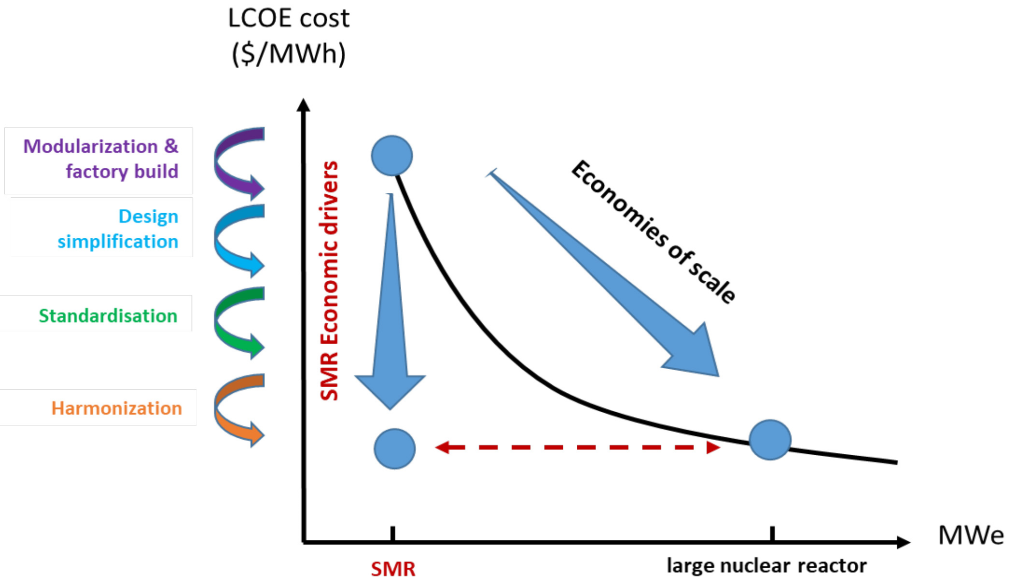
\includegraphics[width=0.8\textwidth]{content/figures/economy.png}
  \caption{Principales impulsores económicos para compensar las desventajas de la pequeña escala de los \acrshortpl{smr} (\cite{nea_smrs_2021}).}
  \label{fig:economy}
\end{figure}

Por último, vale la pena tener en mente los órdenes de magnitud del coste total de un \acrlong{smr}. Para ello, se emplean los resultados detallados a continuación de un estudio económico realizado por la \emph{Energy Policy Institute} de la Universidad de Chicago sobre el VOYGR-12 \acrshort{smr} de la empresa NuScale Power: 

\begin{table}[h]
  \centering
  \resizebox{0.7\textwidth}{!}{%
  \begin{tabular}{|c|c|}
  \hline
  \rowcolor[HTML]{ECF4FF} 
  \textbf{GENERAL DESCRIPTION}                      & \textbf{VOYGR-12 COSTS}  \\ \hline
  \rowcolor[HTML]{9698ED} 
  \textbf{Capitalized Direct Costs}                 & \textbf{\$1,805,616,142} \\ \hline
  \rowcolor[HTML]{CBCEFB} 
  Structures and Improvements                       & \$612,136,797            \\ \hline
  \rowcolor[HTML]{CBCEFB} 
  Reactor Plant Equipment                           & \$869,360,876            \\ \hline
  \rowcolor[HTML]{CBCEFB} 
  Turbine Plant Equipment                           & \$196,121,808            \\ \hline
  \rowcolor[HTML]{CBCEFB} 
  Electric Plant Equipment                          & \$34,982,052             \\ \hline
  \rowcolor[HTML]{CBCEFB} 
  Heat Rejection Systems                            & \$62,934,255             \\ \hline
  \rowcolor[HTML]{CBCEFB} 
  Miscellaneous Plant Equipment                     & \$30,080,354             \\ \hline
  \rowcolor[HTML]{FD6864} 
  \textbf{Capitalized Indirect Costs}               & \textbf{\$663,710,610}   \\ \hline
  \rowcolor[HTML]{FFCCC9} 
  Design Services at Home Office                    & \$130,978,572            \\ \hline
  \rowcolor[HTML]{FFCCC9} 
  Field Construction Management                     & \$60,906,859             \\ \hline
  \rowcolor[HTML]{FFCCC9} 
  Field Construction Supervision                    & \$246,930,385            \\ \hline
  \rowcolor[HTML]{FFCCC9} 
  Field Indirect Costs                              & \$224,894,794            \\ \hline
  \rowcolor[HTML]{FFCE93} 
  \textbf{Total Manufacture and Construction Costs} & \textbf{\$2,469,326,752} \\ \hline
  \end{tabular}%
  }
  \caption{Costes estimados de la fabricación y construcción del VOYGR-12 (\cite{cost_evaluation_nuscale}).}
  \label{tab:costes_voygr-12}
  \end{table}

  El VOYGR-12 \acrshort{smr} es una planta de 924 MWe constituida por 12 módulos de 77 MWe cada uno, por lo que el coste total por unidad de energía generada es de 2.672,43 \$/kWh. Por otro lado, el coste total estimado del reactor AP1000 de Westinghouse ---con una potencia de 1.110 MWe--- es de \$6,8 mil millones (\cite{cost_ap1000}), resultando un coste total por unidad de energía producida de 6.126,13 \$/kWh, 2,3 veces superior que en el caso anterior. En la siguiente tabla se exponen los resultados recopilados, poniéndose de manifiesto la competitividad económica de los reactores modulares pequeños frente a los de gran escala:

  \begin{table}[h]
    \centering
    \resizebox{0.9\textwidth}{!}{%
    \begin{tabular}{
    >{\columncolor[HTML]{FFCCC9}}c |
    >{\columncolor[HTML]{FFFFFF}}c |c|}
    \cline{2-3}
    \cellcolor[HTML]{FFFFFF}\textbf{} &
      \cellcolor[HTML]{ECF4FF}\textbf{AP1000} &
      \cellcolor[HTML]{ECF4FF}\textbf{VOYGR-12 SMR} \\ \hline
    \multicolumn{1}{|c|}{\cellcolor[HTML]{FFCCC9}\textbf{Coste total estimado (\$)}} &
      6.800.000.000 &
      2.469.326.752 \\ \hline
    \multicolumn{1}{|c|}{\cellcolor[HTML]{FFCCC9}\textbf{Coste total por unidad de energía producida (\$/kWh)}} &
      6.126,13 &
      \cellcolor[HTML]{FFFFFF}2.672,43 \\ \hline
    \end{tabular}%
    }
    \caption{Comparación de costes entre una central nuclear de gran escala de generación III+ y un SMR en fase avanzada de desarrollo (\cite{cost_ap1000} y \cite{cost_evaluation_nuscale}).}
    \label{tab:comparacion_voygr_ap1000}
    \end{table}

\newpage

\subsubsection{Diversidad de aplicaciones}

A parte de las mejoras económicas, logísticas y de seguridad, los \acrlongpl{smr} presentan grandes ventajas en múltiples aplicaciones. A continuación se ofrece una explicación genérica de cada una de dichas aplicaciones, ofreciendo una explicación más detallada en el caso del seguimiento de carga (apartado \ref{seguimiento_de_carga}), un modo de operación de gran interés práctico que se pretende simular en el \acrshort{sgiz} en el presente proyecto.

\paragraph{Cogeneración} \label{cogeneracion}

La cogeneración consiste en la producción simultánea de electricidad y calor. Actualmente, esta utilidad de las centrales nucleares ya está siendo explotada en diversos países del mundo, ya que, al aprovechar mejor los recursos generados, se mejora la eficiencia térmica ---hasta un 80\%---, se reducen las emisiones de $CO_2$, $NO_x$ y $SO_2$ asociadas al empleo de combustibles fósiles y, por tanto, aumentan los beneficios económicos. La gran ventaja que introducen los \acrshortpl{smr} a esta práctica es que ---debido a la menor escala, a la versatilidad y a la seguridad de los mismos--- pueden ubicarse mucho más cerca de la población y de los consumidores finales, minimizando los costes y las pérdidas térmicas que derivan del transporte del calor a largas distancias. Además, el desarrollo de reactores de \acrshort{genIV} que trabajan a altas temperaturas aumenta, como se observa en la figura \ref{fig:wna_heat_applications} el abanico de aplicaciones posibles de esta tecnología.

La extracción del calor se lleva a cabo directamente del vapor a media y alta temperatura (300 - 900ºC) a la salida de los generadores de vapor, pudiéndose aprovechar también el vapor a baja temperatura extraído a la salida de la turbina (100 - 200ºC). El calor obtenido puede ser empleado para múltiples aplicaciones, siendo especialmente interesantes la \textbf{calefacción urbana}, la \textbf{desalación} y la \textbf{producción de hidrógeno} termoquímico. 

Por una parte, la carencia de agua dulce en múltiples países es un gran desafío al que se enfrenta nuestra sociedad actual. Según un informe de la \acrshort{onu}, hay alrededor de 4.000 millones de peronas en el mundo ---prácticamente la mitad de la población mundial--- que padecen escasez de agua durante al menos un mes al año (\cite{onu_agua}). A parte de las necesarias mejoras en la distribución y el reciclaje del agua, se hace cada vez más necesaria la construcción de desaladoras que eliminen las sales en exceso del agua del mar y la conviertan en agua dulce apta para el abastecimiento humano. Los dos principales tipos de \textbf{desalación} son la desalación térmica y la ósmosis inversa. En la primera, además de energía eléctrica, se requiere energía térmica para evaporar el agua salada, que será posteriormente condensada en forma de agua dulce. En la ósmosis inversa, se requiere energía eléctrica para bombear el agua a presión y hacerla pasar a través de membranas. Ambas necesidades ---calor y electricidad--- pueden ser cubiertas mediante el empleo de la energía nuclear, razón por la cual numerosos países han apostado  o quieren apostar por la construcción de centrales nucleares junto al mar con capacidad de desalación, o por el uso de la tecnología nuclear para cubrir la demanda térmica y eléctrica requerida para esta aplicación. Tal y como se ha expuesto anteriormente los \acrshortpl{smr} son una opción muy atractiva para este uso por las ventajas que presentan en lo que se refiere a la cogeneración.

Por otra parte, ante la preocupación por la protección del medioambiente y el consecuente propósito de reemplazar a los combustibles fósiles para la reducción de emisiones, el \textbf{hidrógeno} se presenta como una fuente de energía limpia para el transporte, el almacenamiento de energía o la producción de electricidad. La producción de hidrógeno en la actualidad se lleva a cabo principalmente mediante el reformado del metano, proceso que genera elevadas emisiones de $CO_2$. Por tanto, el uso de la tecnología nuclear para la producción de hidrógeno es una alternativa interesante que requiere de un sistema de cogeneración equipado con los compoenentes necesarios para obtener el hidrógeno, principalmente, por electrólisis o mediante procesos termoquímicos. Por un lado, la electrólisis consiste en inducir mediante una corriente eléctrica la división de las moléculas de agua para producir hidrógeno y oxígeno. La electrólisis del agua líquida tiene lugar a temperaturas relativamente bajas ---entre 80 y 120°C---, mientras que la del vapor ocurre a temperaturas mucho más elevadas ---entre 700 y 950ºC--- y es mucho más eficiente. Este último tipo de electrólisis es ideal para producirse mediante reactores nucleares avanzados de altas temperaturas. Por otro lado, la producción de hidrógeno mediante procesos termoquímicos consiste en inducir reacciones químicas con determinados compuestos para dividir ---igual que en la electrólisis--- las moléculas de agua. Para este mecanismo de obtención de hidrógeno también se requieren las elevadas cantidades de calor que son capaces de proporcionar los reactores avanzados de alta temperatura.

En definitiva, dependiendo de la tecnología empleada, del tipo de combustible y de la temperatura alcanzada, la cogeneración nuclear puede emplearse para unas u otras aplicaciones, tal y como se muestra en la siguiente figura:

\begin{figure}[h]
  \centering
  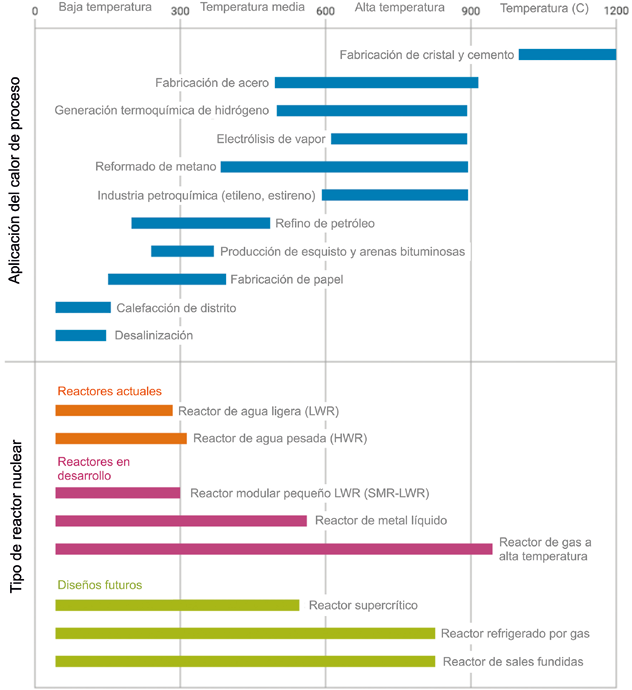
\includegraphics[width=0.71\textwidth]{content/figures/aplicaciones_calor.png}
  \caption{Rangos de temperatura para las distintas aplicaciones con necesidad de calor y tipos de reactores que pueden cubrir esa demanda (\cite{wna_heat_applications}).}
  \label{fig:wna_heat_applications}
\end{figure}

En el gráfico anterior se pone de manifiesto la existencia de múltiples procesos industriales que actualmente emplean combustibles fósiles y que pueden descarbonizarse mediante la cogeneración nuclear y, en concreto, mediante el uso de reactores avanzados para este propósito.

\paragraph{Seguimiento de carga} \label{seguimiento_de_carga}

Tradicionalmente, por razones técnicas y económicas, las centrales nucleares se han empleado para la generación de energía eléctrica como \textbf{centrales base}\footnote{Se denomina ``centrales base'' a aquellas plantas generadoras de elevada potencia cuya función es suministrar energía eléctrica de forma permanente, ofreciendo así un abastecimiento base fiable que cubra gran parte de la demanda eléctrica. Operan durante largos períodos contínuos, evitando en la medida de lo posible las interrupciones. Se incluye en este grupo a las centrales térmicas ---carbón, gas natural\dots---, nucleares e hidráulicas con gran capacidad de generación.}. Desde el punto de vista técnico, es complicado equilibrar las poblaciones neutrónicas del núcleo del reactor, mantener constante la eliminación de calor residual del núcleo y garantizar la integridad física de los compomenentes estructurales, cuando se dan variaciones de temperatura derivadas de las variaciones de potencia requeridas para el seguimiento de carga. Desde el punto de vista económico, debido a los elevados costes de capital inicial y a los reducidos costes de combustible, las centrales nucleares suministran electricidad al menor precio posible cuando mantienen un elevado \gls{factor de carga}, por lo que interesa que funcionen a plena potencia (\cite{stanford_load_following}).

Sin embargo, últimamente ha aumentado el interés en la capacidad de seguimiento de carga de las plantas nucleares, principalmente, en los siguientes dos casos concretos:

\begin{itemize}
  \item Redes eléctricas donde la energía nuclear representa una gran parte de la generación energética total, como es el caso de Francia (63 \%), Ontario (51 \%), Ucrania (56 \%), Carolina del Sur (55 \%), Illinois (52 \%), etc. En estos casos interesa que esta fuente de energía, al ser mayoritaria, tenga capacidad de adaptación a las habituales fluctuaciones de la demanda eléctrica diarias y a lo largo de las distintas épocas del año.
  \item Redes eléctricas donde las fuentes de energía renovable intermitentes ---como la solar y la eólica--- constituyen una parte importante de la producción eléctrica total y presentan importante variaciones en la producción. Algunos casos en los que se da esta segunda situación son Alemania, España, Ontario, Nueva York, California, etc (\cite{ANS_2019}).
\end{itemize} 

Por lo general, se definen tres tipos de maniobras de seguimiento de carga: 

\begin{itemize}
  \item \underline{Regulación primaria de frecuencia:} La demanda de electricidad nunca puede determinarse de antemano con precisión exacta, por lo que existe una cierta variación aleatoria en la demanda que resulta en fluctuaciones de frecuencia generalmente inferiores a 20 mHz. Las centrales nucleares deben monitorear la frecuencia en la red y adaptar inmediatamente su producción para mantener la frecuencia estable en el valor deseado. 
  
  El control de frecuencia primario permite ajustes a corto plazo en la producción de electricidad de acuerdo con la demanda cada 2 - 30 segundos.  En este caso, las correspondientes modulaciones de potencia suelen realizarse dentro de un rango del $\pm 2\%$ de la potencia nominal.
  \item \underline{Regulación secundaria de frecuencia:} Actúa en marcos de tiempo más largos ---desde varios segundos hasta varios minutos--- y restablece la frecuencia exacta calculando una desviación promedio de frecuencia durante un período de tiempo determinado. Con este fin, el operador de la red envía una señal a la central nuclear para modificar su nivel de potencia dentro de un rango del $\pm 5\%$ de la potencia nominal.
  
  \begin{figure}[h]
    \centering
    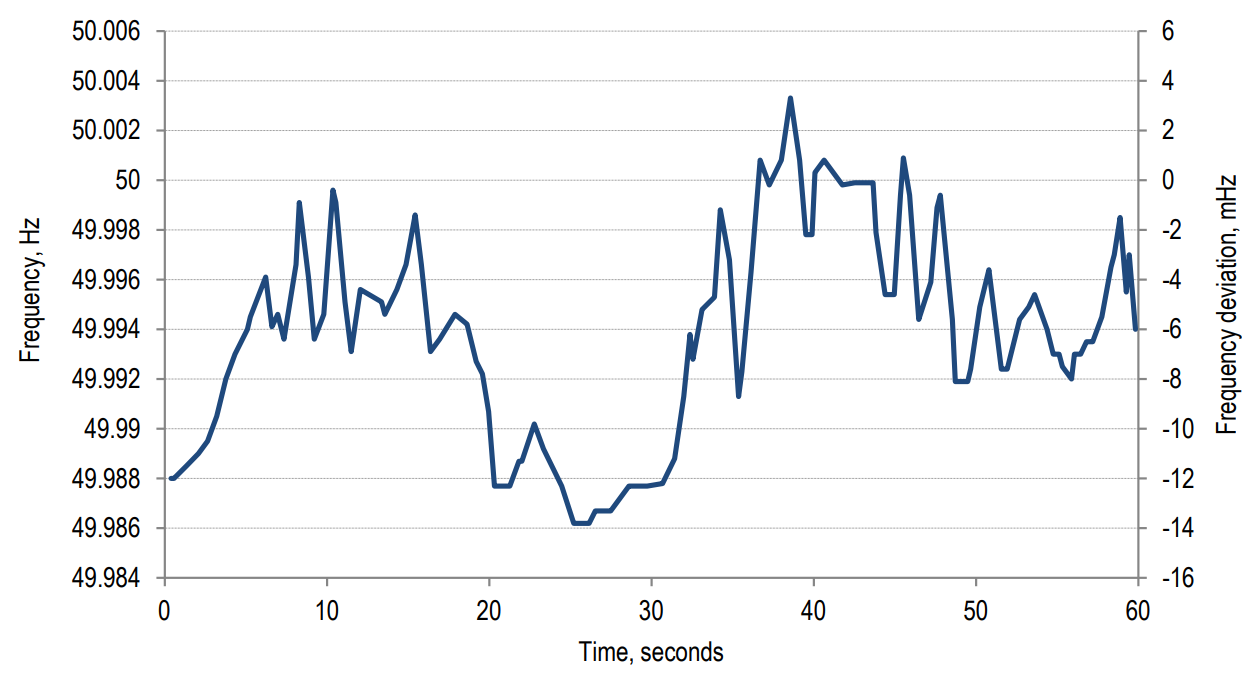
\includegraphics[width=0.7\textwidth]{content/figures/frequency_variation.png}
    \caption{Ejemplo de variaciones en la frecuencia de la red europea (\cite{NEA_2011_load_following}).}
    \label{fig:frequency_variations}
  \end{figure}

  \item \underline{Programas de carga variable predefinidos:} Reducciones o aumentos en la producción de energía acordados previamente con el operador de la red. Se suele tratar de una o dos variaciones de potencia al día, dependiendo de la demanda y de la capacidad de seguimiento de carga de la planta.
  
  \begin{figure}[h]
    \centering
    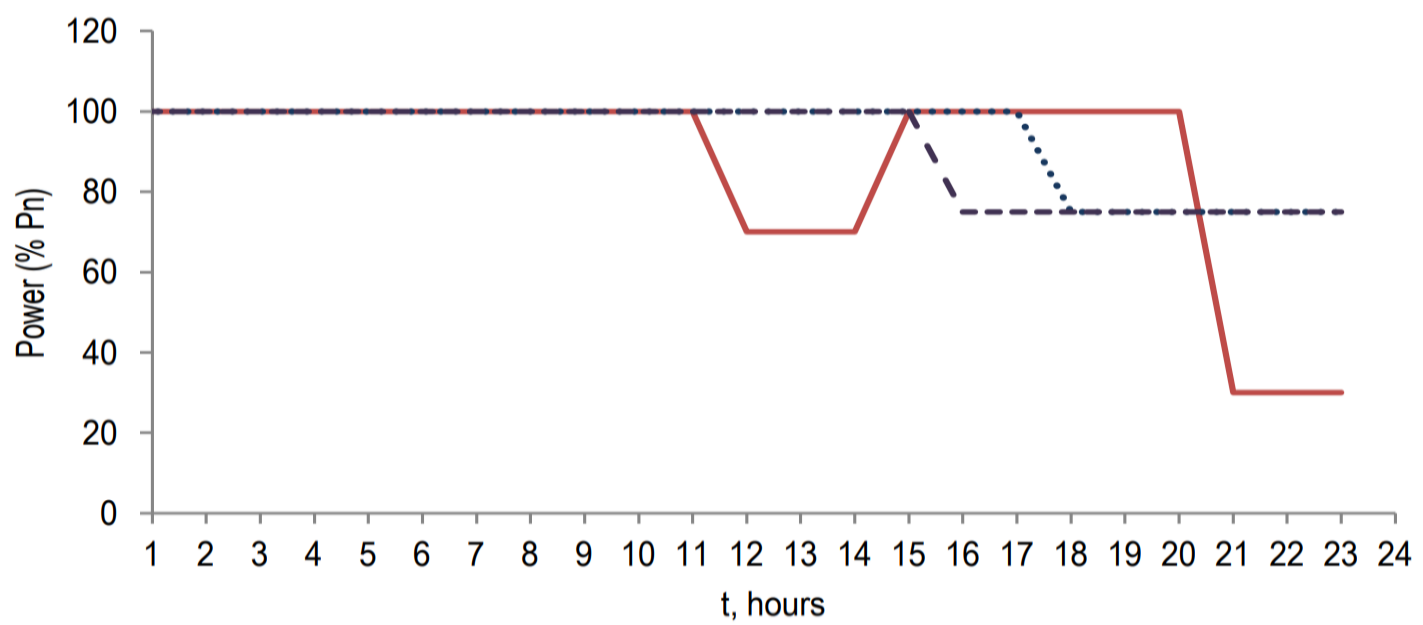
\includegraphics[width=0.7\textwidth]{content/figures/predefined_load_following.png}
    \caption{Ejemplo de un programa de carga variable predefinido para un período de 24 horas, en el que se producen dos reducciones importantes de potencia (\cite{NEA_2011_load_following}).}
    \label{fig:predefined_load_following}
    \vspace{-0.5cm}
  \end{figure}
\end{itemize}

Vale la pena tener en cuenta los órdenes de magnitud que muestran cuantitativamente la capacidad de seguimiento de carga de la mayoría de centrales nucleares de gran escala. Etas, se diseñan con una capacidad de seguimiento de carga similar a la de las centrales de carbón, con unas rampas de potencia de entre 1-5 \%/min y tiempos de arranque hasta alcanzar la potencia total estable del orden de entre un día y varios días. Estas capacidades de seguimiento de carga son mucho más lentas que las de los generadores de las turbinas de gas, que tienen tiempos de arranque de menos de 1 hora y pueden aumentar la potencia a una tasa del 10-20\%/min (\cite{stanford_load_following}).

Centrando ahora la atención en los \acrlongpl{smr}, cabe mencionar que, debido a la incorporación de técnicas de modulación de potencia mejoradas y al diseño de sistemas de control avanzados, tienen mejores capacidades de seguimiento de carga que los hace muy adecuados para operar junto con fuentes de energía renovable intermitentes, contribuyendo así a la estabilidad y flexibilidad del sistema eléctrico. 

En concreto, los niveles de potencia de los pequeños reactores modulares pueden variar entre el \textbf{15 - 100 \%}, con rampas de potencia típicas de \textbf{2 - 5 \%/min}, logrando rampas de potencia de \textbf{10 - 20 \%/min} en algunos diseños (\cite{ANS_2019}). 

\begin{table}[h]
  \centering
  \resizebox{0.7\textwidth}{!}{%
  \begin{tabular}{|
    >{\columncolor[HTML]{FFCCC9}}c |c|c|c|}
    \hline
    \cellcolor[HTML]{ECF4FF}\begin{tabular}[c]{@{}c@{}}Tipo de\\ SMR\end{tabular} &
      \cellcolor[HTML]{ECF4FF}\begin{tabular}[c]{@{}c@{}}Potencia eléctrica\\ (MWe)\end{tabular} &
      \cellcolor[HTML]{ECF4FF}\begin{tabular}[c]{@{}c@{}}Rango de potencia\\ (\%)\end{tabular} &
      \cellcolor[HTML]{ECF4FF}\begin{tabular}[c]{@{}c@{}}Rampa de potencia\\ (\%/min)\end{tabular} \\ \hline
    \textit{\begin{tabular}[c]{@{}c@{}}Pressurized Water Reactor\\ (PWR)\end{tabular}}             & 50 - 160   & 20 - 100 \% & 2 - 5 \\ \hline
    \textit{\begin{tabular}[c]{@{}c@{}}Molten Salt Reactor\\ (MSR)\end{tabular}}                   & 37,5 - 192 & 20 -100 \%  & 5     \\ \hline
    \textit{\begin{tabular}[c]{@{}c@{}}High Temperature Gas-cooled \\ Reactor (HTGR)\end{tabular}} & 76 - 286   & 15 - 100 \% & 5     \\ \hline
    \textit{\begin{tabular}[c]{@{}c@{}}Lead-cooled Fast Reactor\\ (LFR)\end{tabular}}              & 3 - 450    & 0 - 125 \%  & 10    \\ \hline
    \textit{\begin{tabular}[c]{@{}c@{}}Sodium Fast Reactor\\ (SFR)\end{tabular}}                   & 50 - 311   & 20 - 100 \% & 1 - 2 \\ \hline
    \textit{\begin{tabular}[c]{@{}c@{}}Heat Pipe cooled Reactor\\ (HPR)\end{tabular}}              & 0,2 - 25   & 60 - 100 \% & 20    \\ \hline
    \end{tabular}
  }
  \caption{Capacidad de seguimiento de carga de 16 diseños distintos de \acrshortpl{smr} agrupados en el tipo de SMR al que pertenece cada diseño (\cite{ANS_2019}).}
  \label{tab:capacidad_seguimiento_de_carga_smrs}
  \end{table}

A continuación, se detallan los principales métodos existentes para la variación de la potencia y el control de la frecuencia:

\begin{itemize}
  \item \underline{Variación en la concentración de ácido bórico:}\footnote{El ácido bórico es lo que se denomina un ``veneno soluble'' que se disuelve en el refrigerante del reactor y se emplea como un método de control de potencia. El boro es un elemento con elevada sección eficaz de absorción, lo cual disminuye el factor de utilización térmica y ---por la regla de los 4 factores--- disminuye la reactividad del núcleo, disminuyendo de esta manera la potencia generada.} Se emplea en los reactores \acrshort{pwr} y su principal problema de este mecanismo es que se trata de un proceso lento que requiere de varios minutos para tener efecto. Por ello, este método se emplea para los cambios de potencia programados y no para cambios rápidos, para los cuales son más apropiados los dos métodos que se detallan a continuación. Obviamente, también puede usarse este método para variaciones de potencia no programadas, siempre y cuando el tiempo requerido para las mismas sea de, al menos, unos minutos.
  
  \item \underline{Empleo de bancos especiales de las barras de control:} 
  Se trata, concretamente, de los bancos de barras de control A, B, C y D, los cuales se denominan ``bancos de control u operación''.

  Están presentes en todos los tipos de reactores, siendo la forma más común de ajustar la potencia. Las ventajas que presenta el empleo de las barras de control es que ofrecen una respuesta rápida y pueden adaptarse a sistemas de control automático. Sin embargo, producen una distorsión en la distribución de potencia, ya que se agota más el combustible en la parte inferior del reactor que en la parte superior, por donde se insertan dichas barras en el caso de los \acrshortpl{pwr}. Lo bueno es que este problema puede corregirse variando la concentración de ácido bórico y retirando después las barras de control (\cite{apuntes_centrales}).

  \item \underline{Empleo del coeficiente de temperatura del moderador:} Este coeficiente representa la variación de la reactividad con la temperatura del moderador: 
  
  \begin{equation}
    \alpha_{mod}=\frac{\partial \rho}{\partial T_{mod}}
  \end{equation}

  Un reactor, para ser intrínsecamente estable ---y, por tanto, seguro---, debe tener un coeficiente de potencia negativo, de modo que un aumento en la reactividad del núcleo conlleve una reducción de la potencia, tal y como se muestra a continuación:

  \begin{equation} \label{coeficiente_potencia}
    \frac{\partial \rho}{\partial P}=\frac{\partial \rho}{\partial T_c} \frac{\partial T_c}{\partial P}+\frac{\partial \rho}{\partial T_{\mathrm{mod}}} \frac{\partial T_{\mathrm{mod}}}{\partial P}=\alpha_{T c} \frac{\partial T_c}{\partial P}+\alpha_{\mathrm{mod}} \frac{\partial T_{\mathrm{mod}}}{\partial P}<0
  \end{equation}

  Para ello, es necesario que el coeficiente Doppler ($\alpha_{T_{c}}$) y el coeficiente de temperatura del moderador ($\alpha_{mod}$) sean negativos. En un reactor con coeficiente de temperatura del moderador negativo ---para lo cual debe diseñarse para operar en régimen de submoderación---, un aumento de temperatura del moderador conlleva una disminución de la reactividad y, por la ecuación \ref{coeficiente_potencia}, una consecuente disminución de la potencia. De esta manera, aumentando la temperatura del moderador o sobrerefrigerando el núcleo se disminuye o aumenta, respectivamente, la potencia de la planta (\cite{apuntes_centrales}).
  
  Las ventajas que presenta este método es que no hace uso de materiales que puedan desgastarse y que proporciona una potencia homogénea en todo el reactor. Sin embargo, si los cambios de potencia ---y, por tanto, de temparatura--- son muy bruscos, será necesario un presionador lo suficientemente grande como para adaptar la presión del circuito primario a los cambios del nivel de agua producidos (\cite{seguimiento_carga_josep_rey}).
\end{itemize}

En la siguiente figura se muestra una operación de variación de potencia en que se emplean los dos primeros métodos explicados:

\begin{figure}[h]
  \centering
  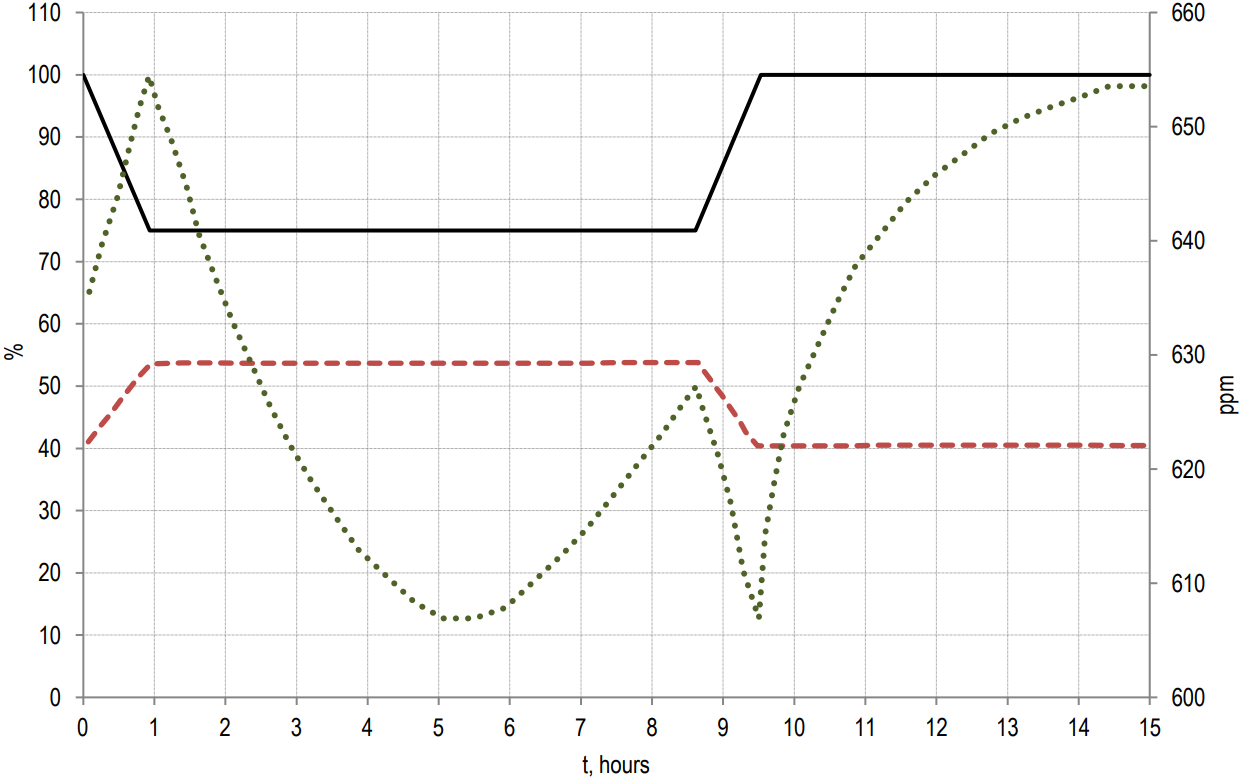
\includegraphics[width=0.7\textwidth]{content/figures/seguimiento_carga_barras_y_boro.png}
  \caption{Ejemplo de variación de potencia mediante la inserción del banco de barras de control D y la variación de la concentración de ácido bórico en un reactor \acrshort{pwr} (\cite{NEA_2011_load_following}).}
  \label{fig:seguimiento_carga_barras_y_boro}
\end{figure}

Tal y como se ha comentado al inicio de este subapartado, es preferible mantener el reactor operando constantemente a su máxima potencia, evitando así el ciclado térmico de los componentes del núcleo del reactor y del circuito primario. Por eso, los diseños de \acrshort{smr} más recientes apuestan principalmente por mantener siempre el circuito primario de la planta a plena potencia y seguir la curva de carga utilizando la energía ---tanto térmica como eléctrica--- del lado secundario para la cogeneración Una opción muy atractiva es la \textbf{derivación de vapor/turbina}. Cuando la demanda de electricidad en la red eléctrica cambia, el operador de la central puede ajustar la cantidad de vapor que pasa a través de la turbina principal utilizando válvulas de derivación. Al abrirlas, parte del vapor se desvía y no pasa por la turbina, lo que reduce la cantidad de energía que se convierte en electricidad (\cite{ANS_2019}). Este vapor puede emplearse para disintos fines, como calefacción urbana, desalación, producción de hidrógeno, etc. tal y como se detalla en el apartado de \textit{Cogeneración (\ref{cogeneracion})}. 

\paragraph{Abastecimiento de zonas remotas}

Las grandes centrales nucleares tienen un papel importante en el mix energético de muchos países como centrales base, ofreciendo una elevada garantía de suministro en sistemas eléctricos centralizados e interconectados. Sin embargo, el desarrollo de estos grandes reactores es muy reducido en regiones donde las limitaciones económicas, geográficas o relacionadas con la red eléctrica, dificultan la viabilidad de su construcción. 

Frente a esta realidad, la modularidad, flexibilidad, reducción de tiempos de construcción y costes, y los bajos requisitos de red de los \acrlongpl{smr}, convierten a esta tecnología avanzada en una posible solución al necesario abastecimiento eléctrico de áreas remotas que no están conectadas a la red, regiones con redes eléctricas pequeñas o regiones que no pueden permitirse la construcción de grandes centrales. A continuación se detallan algunos casos concretos en los que la tecnología \acrshort{smr} puede resultar muy adecuada:

\begin{itemize}
  \item La \textbf{pobreza energética} es una realidad en muchos países del mundo. Un ejemplo claro y destacado es el continente africano, donde, en la actualidad, 600 millones de personas ---el 43\% de la población total--- carecen de acceso a la electricidad, la mayoría de ellos pertenecientes a países del África subsahariana (\cite{iea_africa}). 
  
  Distintos organismos, empresas y desarrolladores están promoviendo el uso de los pequeños reactores modulares para, o bien abastecer ---junto con las fuentes de energía renovable--- de forma independiente zonas remotas que no están conectadas a la red, o bien desarrollar en determinados países un sistema eléctrico más interconectado que permita la construcción de múltiples \acrshortpl{smr} para cubrir, junto con otras fuentes de energía, la demanda energética total. Por ejemplo, un estudio realizado por un grupo de ingenierios y físicos nucleares de la Universidad de Johannesbrugo, analiza y propone un despliegue nuclear gradual a gran escala de 700 \acrshortpl{smr} de tipo \acrshort{htgr} para cubrir el déficit energético de los países del África subsahariana, que han estimado que podría conseguirse añadiendo una capacidad instalada de 68 GW  (\cite{application_smrs_africa}). 
  
  Por otro lado, muchos países de África están desarrollando o pretenden desarrollar un programa nuclear enfocado, en algunos casos, en la construcción de reactores tanto de gran como de pequeña escala. Tal y como se observa en la figura \ref{fig:africa_nuclear_support}, algunos países van más avanzados en este camino, mientras que otros todavía tienen por delante mucho trabajo de impulso económico y político, formación de personal, creación de las empresas y el organismo regulador necesario, etc.

  \begin{figure}[h]
    \centering
    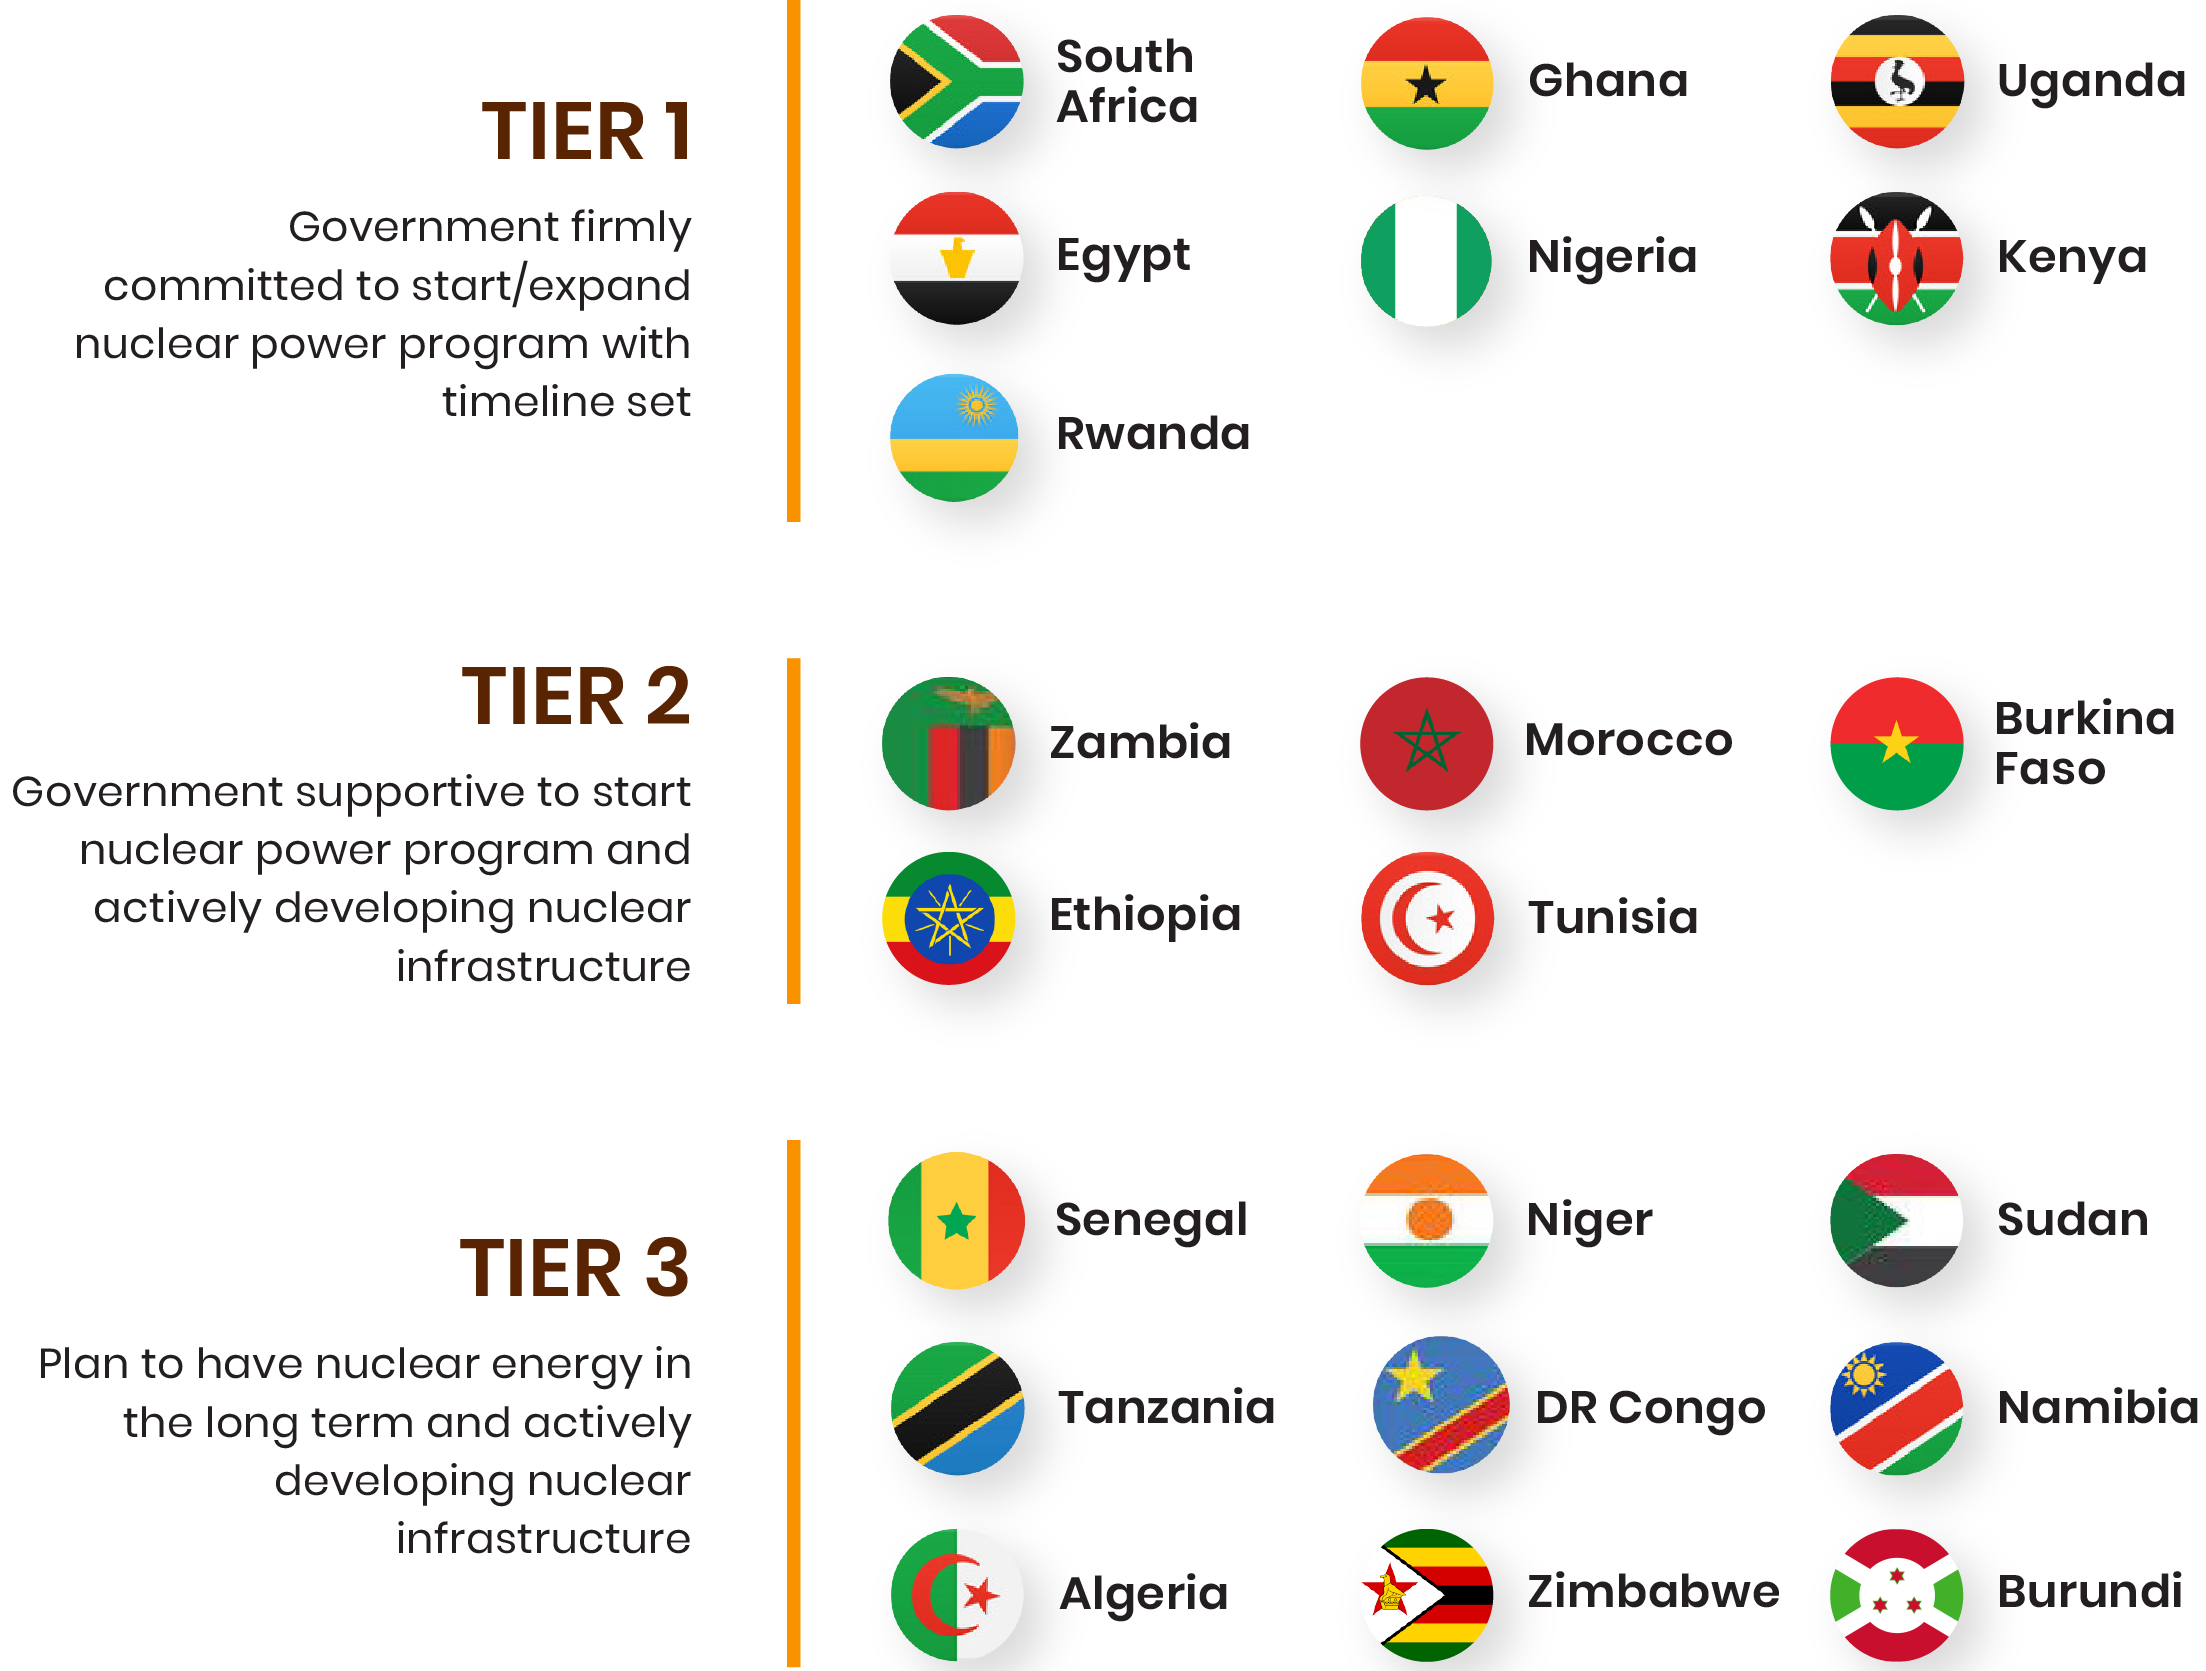
\includegraphics[width=0.75\textwidth]{content/figures/africa_nuclear_support.png}
    \caption{Países de África implicados en incorporar la energía nuclear en su mix energético divididos en 3 niveles, según el grado de avance (\cite{nba_africa}).}
    \label{fig:africa_nuclear_support}
  \end{figure}

  \item Por otra parte, existen usos muy específicos en áreas remotas para los que el uso de generadores diésel podría reemplazarse por reactores modulares pequeños y, en concreto, por microrreactores (\acrshort{mmr}). Es el caso de las \textbf{comunidades mineras} o de las \textbf{bases militares} aisladas, por ejemplo.
  
  \item En relación con el punto anterior, los \acrshortpl{smr} de muy pequeña escala también resultan muy atractivos para aplicaciones espaciales, tal y como se explica con más detalle en el siguiente apartado. 
\end{itemize}

\paragraph{Exploración espacial} \label{exploracion_espacial}

Una última aplicación que se va detallar en este análisis es el empleo de reactores nucleares de pequeña escala para misiones espaciales, principalmente, con los siguientes dos objetivos:

\begin{itemize}
  \item \underline{Propulsión de naves espaciales:} Consiste en sustituir o apoyar, mediante motores nucleares, los motores químicos que se han usado tradicionalmente en la propulsión espacial. Existen dos principales tecnologías para este propósito:
  \begin{itemize}
    \item \textbf{Propulsión termonuclear (\acrshort{ntp}):} Consiste en transferir calor desde el reactor a un propelente líquido ---como puede ser el hidrógeno---. Este calor convierte el líquido en gas, el cual se expande a través de una tobera para proporcionar el empuje necesario para propulsar a la nave espacial. Esta tecnología proporciona un empuje elevado y el doble de eficiencia en el consumo de propelente en comparación con los cohetes químicos, permitiendo una carga menor de combustible y una reducción considerable de tiempos de viaje ---se estima una reducción del 25\%---.
    
    \begin{figure}[h]
      \centering
      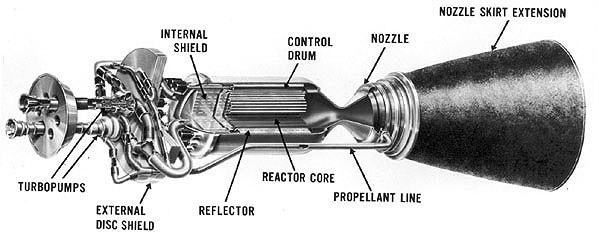
\includegraphics[width=0.7\textwidth]{content/figures/rover_nerva_engine.jpg}
      \caption{Diseño de un \acrfull{nerva} (\cite{nasa_space_nuclear_propulsion}).}
      \label{fig:nasa_space_nuclear_propulsion}
    \end{figure}

    \item \textbf{Propulsión electronuclear (\acrshort{nep}):} Consiste en utilizar un reactor para generar electricidad que carga positivamente los propelentes gaseosos y empuja los iones a través de un propulsor, lo que impulsa la nave espacial hacia adelante. Los sistemas \acrshort{nep} proporcionan bajo empuje pero continuo y utilizan los propelentes de manera mucho más eficiente que los cohetes químicos, aumentando mucho la velocidad y reduciendo así mucho los tiempos de viaje ---se estima una reducción superior al 60\%---.
  \end{itemize}

  Actualmente, la \acrshort{nasa} está llevando a cabo varios programas de investigación sobre diversas opciones para propulsar naves espaciales mediante energía nuclear. Cabe destacar el proyecto Kilopower, que emprendió en 2017 con apoyo del Departamento de Energía de los EEUU. El proyecto consiste en el diseño de un reactor  que, junto con un motor Stirling, proporciona una potencia eléctrica de entre 1 y 10 kWe que alimenta el generador eléctrico de la aeronave, el cual aplica un elevado voltaje a una corriente de Xe para ionizarlo y generar un plasma que, al ser acelerado, propulse la nave (\cite{nasa_space_nuclear_propulsion}).

  \item \underline{Generación de energía en superfície extraterrestre:} Se están llevando a cabo proyectos para emplear \acrshortpl{mmr} como fuente de energía fiable para misiones espaciales de exploración que requieran una permanencia prolongada en otros planetas. Estas unidades serían fabricadas en la Tierra y se transportarían al emplazamiento deseado, pudiendo ser operadas de forma remota y con capacidad de albergar astronautas o emplearse como estaciones de exploración remotas.
  
  Cabe destacar a este respecto el reactor del proyecto Kilopower ---mencionado en el punto anterior---, diseñado con capacidad de suministro de 10 kWe durante 10 años, para futuras misiones tripuladas en la Luna o en Marte (\cite{nasa_fission_surface_power}).
  
\end{itemize}

\newpage
\subsection{Clasificación de los Small Modular Reactors}

Pese a que existen diversos criterios para determinar los distintos tipos de \acrshortpl{smr}, en el presente proyecto se ha escogido la clasificación realizada por el \acrshort{oiea}, en la que se distinguen 6 grupos, de los cuales se ofrece a continuación una descripción y las tecnologías concretas desarrolladas:

\subsubsection{SMRs refrigerados por agua establecidos en tierra}

 Utilizan varias configuraciones de reactores de agua ligera (del inglés, \acrshortpl{lwr}) y de reactores de agua pesada (del inglés, \acrshortpl{hwr}) para establecerse en tierra y con posibilidad de aplicaciones sin conexión a la red. Se trata de la tecnología de \acrshort{smr} más madura en la actualidad, ya que la mayoría de las centrales nucleares de gran potencia en operación actualmente también son refrigeradas por agua.

 \begin{table}[h]
  \resizebox{\textwidth}{!}{%
  \begin{tabular}{|
  >{\columncolor[HTML]{FFCCC9}}c |c|c|c|c|c|}
  \hline
  \cellcolor[HTML]{ECF4FF}\textbf{Diseño} &
    \cellcolor[HTML]{ECF4FF}\textbf{Potencia (MWe)} &
    \cellcolor[HTML]{ECF4FF}\textbf{Tipo} &
    \cellcolor[HTML]{ECF4FF}\textbf{Diseñador} &
    \cellcolor[HTML]{ECF4FF}\textbf{País} &
    \cellcolor[HTML]{ECF4FF}\textbf{Estado} \\ \hline
  CAREM &
    30 &
    \acrshort{pwr} &
    CNEA &
    Argentina &
    En construcción \\ \hline
  ACP100 &
    125 &
    \acrshort{pwr} &
    CNNC/NPIC &
    China &
    En construcción \\ \hline
  CANDU SMR$^{TM}$ &
    300 &
    \acrshort{phwr} &
    Candu Energy &
    Canadá &
    Diseño conceptual \\ \hline
  CAP200 &
    \textgreater 200 &
    \acrshort{pwr} &
    SPIC/SNERDI &
    China &
    Diseño básico \\ \hline
  DHR400 &
    400 MWt &
    \acrshort{pwr} &
    CNNC &
    China &
    Diseño básico \\ \hline
  HAPPY200 &
    200 MWt &
    \acrshort{pwr} &
    SPIC &
    China &
    Diseño detallado \\ \hline
  NHR200-II &
    200 MWt &
    \acrshort{pwr} &
    Tsinghua University &
    China &
    Diseño básico \\ \hline
  TEPLATOR$^{TM}$ &
    \textless 150 MWt &
    \acrshort{hwr} &
    \begin{tabular}[c]{@{}c@{}}UWB Pilsen \\ \& CIIRC CTU\end{tabular} &
    República checa &
    Diseño conceptual \\ \hline
  NUWARD$^{TM}$ &
    2 × 170 &
    \acrshort{pwr} &
    EDF &
    Francia &
    Diseño conceptual \\ \hline
  IMR &
    350 &
    \acrshort{pwr} &
    MHI &
    Japón &
    \begin{tabular}[c]{@{}c@{}}Diseño conceptual\\ completado\end{tabular} \\ \hline
  i-SMR &
    170 &
    \acrshort{pwr} &
    \begin{tabular}[c]{@{}c@{}}KHNP \&\\ KAERI\end{tabular} &
    República de Corea &
    Diseño conceptual \\ \hline
  SMART &
    107 &
    \acrshort{pwr} &
    \begin{tabular}[c]{@{}c@{}}KAERI \\ \& K.A.CARE\end{tabular} &
    \begin{tabular}[c]{@{}c@{}}República de Corea\\ y Arabia Saudí\end{tabular} &
    Diseño detallado \\ \hline
  RITM-200N &
    55 &
    \acrshort{pwr} &
    \begin{tabular}[c]{@{}c@{}}JSC Afrikantov\\ \& OKBM Rosatom\end{tabular} &
    Rusia &
    \begin{tabular}[c]{@{}c@{}}Diseño detallado\\ completado\end{tabular} \\ \hline
  VK-300 &
    250 &
    \acrshort{bwr} &
    NIKIET &
    Rusia &
    Diseño detallado \\ \hline
  KARAT-45 &
    45 – 50 &
    \acrshort{bwr} &
    NIKIET &
    Rusia &
    Diseño conceptual \\ \hline
  KARAT-100 &
    100 &
    \acrshort{bwr} &
    NIKIET &
    Rusia &
    Diseño conceptual \\ \hline
  RUTA-70 &
    70 MWt &
    \acrshort{pwr} &
    NIKIET &
    Rusia &
    Diseño conceptual \\ \hline
  STAR &
    10 &
    \acrshort{pwr} &
    STAR ENERGY &
    Suiza &
    Diseño básico \\ \hline
  Rolls-Royce SMR &
    470 &
    \acrshort{pwr} &
    Rolls-Royce &
    Reino Unido &
    Diseño detallado \\ \hline
  VOYGR$^{TM}$ &
    4/6/12 × 77 &
    \acrshort{pwr} &
    NuScale Power &
    EEUU &
    \begin{tabular}[c]{@{}c@{}}Fabricación de\\ equipos en proceso\end{tabular} \\ \hline
  BWRX-300 &
    270 – 290 &
    \acrshort{bwr} &
    Hitachi &
    EEUU y Japón &
    Diseño detallado \\ \hline
  SMR-160 &
    160 &
    \acrshort{pwr} &
    Holtec International &
    EEUU &
    \begin{tabular}[c]{@{}c@{}}Diseño preliminar\\ completado\end{tabular} \\ \hline
  Westinghouse SMR &
    \textgreater 225 &
    \acrshort{pwr} &
    Westinghouse &
    EEUU &
    \begin{tabular}[c]{@{}c@{}}Diseño conceptual\\ completado\end{tabular} \\ \hline
  mPower &
    2 × 195 &
    \acrshort{pwr} &
    BWX Technologies &
    EEUU &
    Diseño conceptual \\ \hline
  OPEN20 &
    22 &
    \acrshort{pwr} &
    Last Energy &
    EEUU &
    Diseño detallado \\ \hline
  \end{tabular}%
  }
  \caption{Diseños existentes de SMRs refrigerados por agua establecidos en tierra (\cite{iaea_smr_booklet_2022}).}
  \label{tab:smrs_agua_tierra}
  \end{table}

\subsubsection{SMRs refrigerados por agua establecidos en el mar}

Instalaciones flotantes montadas en barcos o sumergidas bajo el mar. Ofrecen una gran versatilidad gracias a su capacidad de desplazamiento. A este grupo pertenecen los dos reactores KLT-40S pertenecientes a la \textbf{planta de energía nuclear flotante Akademik Lomonosov}, que comenzó su operación comercial en Pevek (Rusia) en mayo de 2020, siendo \textbf{el primer diseño de SMR conectado a la red}, con una potencia eléctrica total ---entre ambos reactores--- de 70 MWe y 300 MWt, proporcionando así electricidad a una ciudad de 100.000 habitantes.

\begin{figure}[h]
    \centering
    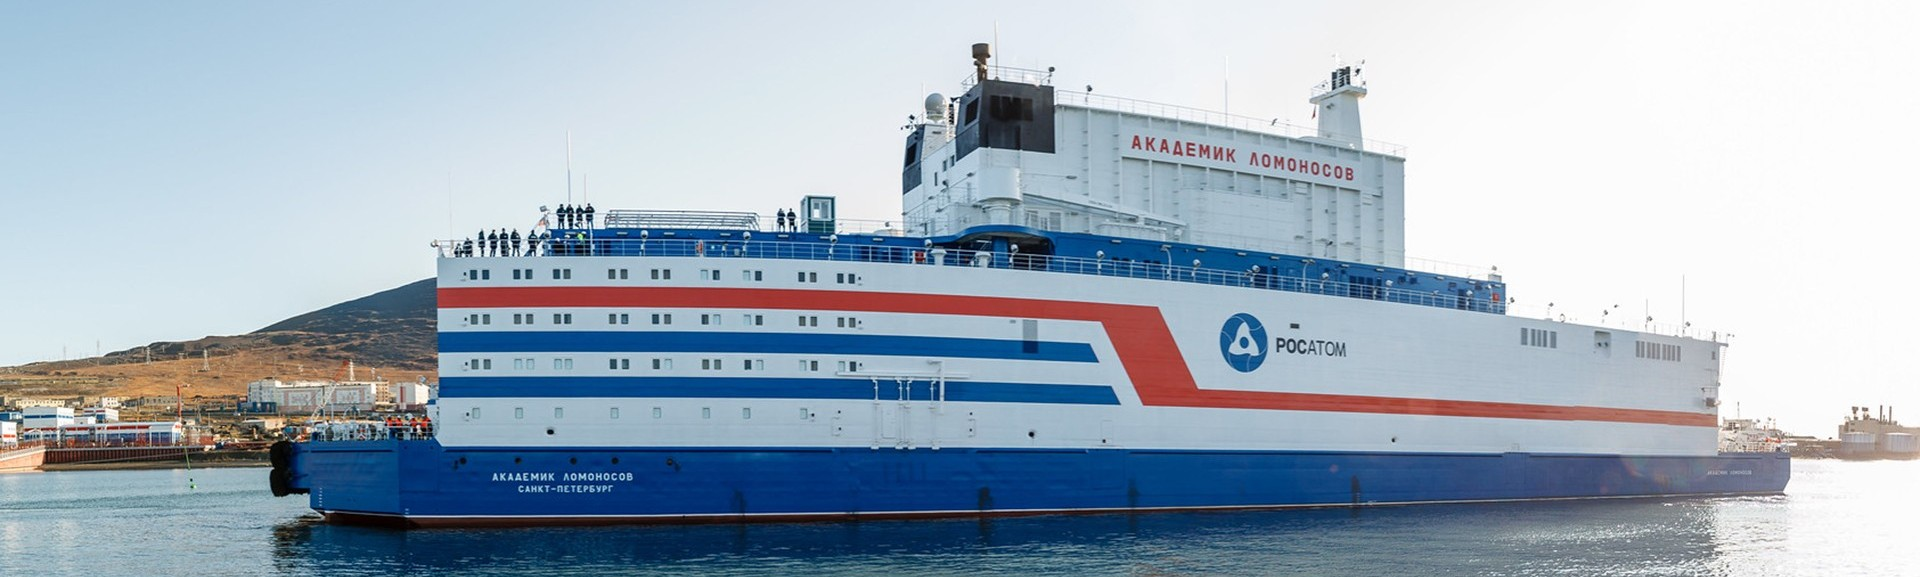
\includegraphics[width=0.8\textwidth]{content/figures/akademik_lomonosov.jpg}
    \caption{La central nuclear flotante Akademik Lomonosov (\cite{nuclear_españa}).}
    \label{fig:akademik_lomonosov}
\end{figure}

\begin{table}[h]
  \resizebox{\textwidth}{!}{%
  \begin{tabular}{|
  >{\columncolor[HTML]{FFCCC9}}c |c|c|c|c|c|}
  \hline
  \cellcolor[HTML]{ECF4FF}\textbf{Diseño} &
    \cellcolor[HTML]{ECF4FF}\textbf{Potencia (MWe)} &
    \cellcolor[HTML]{ECF4FF}\textbf{Tipo} &
    \cellcolor[HTML]{ECF4FF}\textbf{Diseñador} &
    \cellcolor[HTML]{ECF4FF}\textbf{País} &
    \cellcolor[HTML]{ECF4FF}\textbf{Estado} \\ \hline
  KLT-40S &
    2 × 35 &
    \acrshort{pwr} &
    JSC Afrikantov OKBM &
    Rusia &
    En operación \\ \hline
  ACPR50S &
    50 &
    \acrshort{pwr} &
    CGNPC &
    China &
    Diseño detallado \\ \hline
  ACP100S &
    125 &
    \acrshort{pwr} &
    CNNC/NPIC &
    China &
    Diseño básico \\ \hline
  BANDI-60 &
    60 &
    \acrshort{pwr} &
    KEPCO E\&C &
    Corea del Sur &
    Diseño conceptual \\ \hline
  ABV-6E &
    6 – 9 &
    \acrshort{pwr} &
    \begin{tabular}[c]{@{}c@{}}JSC Afrikantov\\ OKBM, Rosatom\end{tabular} &
    Rusia &
    Diseño final \\ \hline 
  RITM-200M &
    50 &
    \acrshort{pwr} &
    \begin{tabular}[c]{@{}c@{}}JSC Afrikantov\\ OKBM, Rosatom\end{tabular} &
    Rusia &
    \begin{tabular}[c]{@{}c@{}}Diseño básico\\ completado\end{tabular} \\ \hline
  VBER-300 &
    325 &
    \acrshort{pwr} &
    \begin{tabular}[c]{@{}c@{}}JSC Afrikantov\\ OKBM, Rosatom\end{tabular} &
    Rusia &
    \begin{tabular}[c]{@{}c@{}}Fase de \\ licenciamiento\end{tabular} \\ \hline
  SHELF-M &
    \textgreater \space 10 &
    \acrshort{pwr} &
    NIKIET &
    Rusia &
    Diseño básico \\ \hline
  \end{tabular}%
  }
  \caption{Diseños existentes de SMRs refrigerados por agua establecidos en el mar (\cite{iaea_smr_booklet_2022}).}
  \label{tab:smrs_agua_mar}
  \end{table}

\subsubsection{SMRs refrigerados por gas de alta temperatura (del inglés, HTGR)}

Reactores de \acrshort{genIV} que proporcionan calor a elevada temperatura (superior a 750°C) y que pueden ser utilizados para generar electricidad de forma más eficiente y con una variedad de aplicaciones industriales. Dentro de esta categoría, hay múltiples diseños en desarrollo y alguno en operación, como el \textbf{HTR-PM de China, el primer \acrshort{htgr} en operación del mundo}. Con un \gls{reactor de lecho de bolas}\footnote{Reactor de muy alta temperatura moderado con grafito y refrigerado por gas, cuyos elementos de combustible son esféricos (denominados ``bolas'') y contienen miles de partículas \acrshort{triso}. Estos combustibles tri-isotrópicos constan de carburo de uranio revestido con varias capas de carbón pirolítico y dióxido de silicio para retener los productos de fisión a altas temperaturas.}, una potencia eléctrica de 210 MWe y una potencia térmica de 500 MWt, se conectó a la red en diciembre de 2021 y comenzó a operar comercialmente a plena potencia en diciembre de 2023, con el objetivo de reemplazar las centrales de carbón presentes en el interior de China. También se incluyen en este grupo tres reactores de prueba \acrshort{htgr}, dos de los cuales han estado en operación durante más de veinte años para realizar pruebas en Japón y China.

\begin{figure}[h]
  \centering
  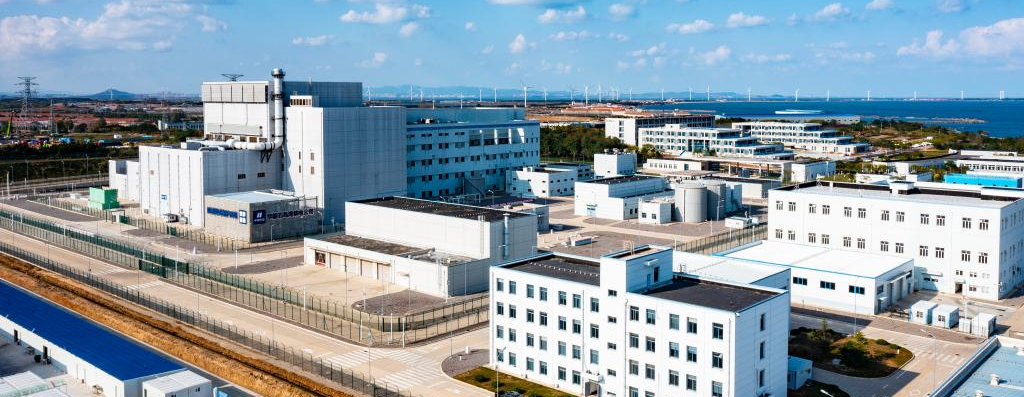
\includegraphics[width=0.65\textwidth]{content/figures/HTR_PM_china.jpg}
  \caption{Primer reactor de \acrshort{genIV} en operación: HTR-PM de China (\cite{htr_pm_china}).}
  \label{fig:htr_pm_china}
\end{figure}

\begin{table}[h]
  \centering
  \resizebox{0.91\textwidth}{!}{%
  \begin{tabular}{|
  >{\columncolor[HTML]{FFCCC9}}c |c|c|c|c|c|}
  \hline
  \cellcolor[HTML]{ECF4FF}\textbf{Diseño} &
    \cellcolor[HTML]{ECF4FF}\textbf{Potencia (MWe)} &
    \cellcolor[HTML]{ECF4FF}\textbf{Tipo} &
    \cellcolor[HTML]{ECF4FF}\textbf{Diseñador} &
    \cellcolor[HTML]{ECF4FF}\textbf{País} &
    \cellcolor[HTML]{ECF4FF}\textbf{Estado} \\ \hline
  HTR-PM &
    210 &
    \begin{tabular}[c]{@{}c@{}}\acrshort{htgr}\\ (lecho de bolas)\end{tabular} &
    \begin{tabular}[c]{@{}c@{}}INET, Tsinghua\\ University\end{tabular} &
    China &
    En operación \\ \hline
  STARCORE &
    14/20/60 &
    \begin{tabular}[c]{@{}c@{}}\acrshort{htgr}\\ (prismático)\end{tabular} &
    StarCore Nuclear &
    Canadá &
    Diseño preconceptual \\ \hline
  JIMMY &
    \begin{tabular}[c]{@{}c@{}}10 – 20\\ MWt\end{tabular} &
    \begin{tabular}[c]{@{}c@{}}\acrshort{htgr}\\ (prismático)\end{tabular} &
    JIMMY ENERGY SAS &
    Francia &
    Diseño detallado \\ \hline
  GTHTR300 &
    100 – 300 &
    \begin{tabular}[c]{@{}c@{}}\acrshort{htgr}\\ (prismático)\end{tabular} &
    JAEA Consortium &
    Japón &
    Diseño básico \\ \hline
  GT-MHR &
    288 &
    \begin{tabular}[c]{@{}c@{}}\acrshort{htgr}\\ (prismático)\end{tabular} &
    JSC Afrikantov OKBM &
    Rusia &
    \begin{tabular}[c]{@{}c@{}}Diseño preliminar\\ completado\end{tabular} \\ \hline
  MHR-T &
    4 × 205,5 &
    \acrshort{htgr} &
    JSC Afrikantov OKBM &
    Rusia &
    Diseño conceptual \\ \hline
  MHR-100 &
    25 – 87 &
    \acrshort{htgr} &
    JSC Afrikantov OKBM &
    Rusia &
    Diseño conceptual \\ \hline
  AHTR-100 &
    50 &
    \begin{tabular}[c]{@{}c@{}}\acrshort{htgr}\\ (lecho de bolas)\end{tabular} &
    Eskom Holdings SOC &
    Sudáfrica &
    \begin{tabular}[c]{@{}c@{}}Diseño conceptual\\ completado\end{tabular} \\ \hline
  PBMR-400 &
    165 &
    \begin{tabular}[c]{@{}c@{}}\acrshort{htgr}\\ (lecho de bolas)\end{tabular} &
    PBMR SOC &
    Sudáfrica &
    \begin{tabular}[c]{@{}c@{}}Diseño preliminar\\ completado\end{tabular} \\ \hline
  HTMR100 &
    35 &
    \begin{tabular}[c]{@{}c@{}}\acrshort{htgr}\\ (lecho de bolas)\end{tabular} &
    STL Nuclear (Pty) &
    Sudáfrica &
    Diseño básico \\ \hline
  EM$^2$ &
    265 &
    \acrshort{gfr} &
    General Atomics &
    EEUU &
    Diseño conceptual \\ \hline
  FMR &
    50 &
    \acrshort{gfr} &
    General Atomics &
    EEUU &
    Diseño conceptual \\ \hline
  Xe-100 &
    82,5 &
    \begin{tabular}[c]{@{}c@{}}\acrshort{htgr}\\ (lecho de bolas)\end{tabular} &
    X-Energy LLC &
    EEUU &
    Diseño básico \\ \hline
  SC-\acrshort{htgr} &
    272 &
    \begin{tabular}[c]{@{}c@{}}\acrshort{htgr}\\ (prismático)\end{tabular} &
    Framatome &
    EEUU &
    Diseño preliminar \\ \hline
  PeLUIt / RDE &
    40 MWt &
    \begin{tabular}[c]{@{}c@{}}\acrshort{htgr}\\ (lecho de bolas)\end{tabular} &
    BRIN &
    Indonesia &
    Diseño conceptual \\ \hline
  HTR-10 &
    2,5 &
    \begin{tabular}[c]{@{}c@{}}\acrshort{htgr}\\ (lecho de bolas)\end{tabular} &
    \begin{tabular}[c]{@{}c@{}}INET, Tsinghua\\ University\end{tabular} &
    China &
    Operable \\ \hline
  HTTR &
    30 MWt &
    \begin{tabular}[c]{@{}c@{}}HT\acrshort{htgr}GR\\ (prismático)\end{tabular} &
    JAEA &
    Japón &
    En operación \\ \hline
  \end{tabular}%
  }
  \caption{Diseños existentes de SMRs refrigerados por gas de alta temperatura (\cite{iaea_smr_booklet_2022}).}
  \label{tab:smrs_gas_alta_temp}
  \end{table}

\newpage

\subsubsection{SMRs rápidos refrigerados por metal líquido (del inglés, LMFR)}

Los metales líquidos que utilizan como regrigerantes incluyen sodio, plomo puro y eutéctico de plomo-bismuto. Hay grandes avances en el desarrollo y despliegue de esta tecnología de \acrshortpl{lmfr}. Prueba de ello es el BREST-OD-300, un reactor de neutrones rápidos refrigerado por plomo que se está construyendo en Seversk (Rusia) y se planea su puesta en marcha en 2026. Se trata de un proyecto prototipo para futuros diseños que empleen un ciclo combustible nuclear cerrado, en el cual pueda reutilizarse el combustible gastado mediante la separación del uranio, plutonio y actínidos minoritarios (Np, Am y Cm), para ser transmutados en estos reactores rápidos (\cite{apuntes_centrales}).

\begin{table}[h]
  \resizebox{\textwidth}{!}{%
  \begin{tabular}{|
  >{\columncolor[HTML]{FFCCC9}}c |c|c|c|c|c|}
  \hline
  \cellcolor[HTML]{ECF4FF}\textbf{Diseño} &
    \cellcolor[HTML]{ECF4FF}\textbf{Potencia (MWe)} &
    \cellcolor[HTML]{ECF4FF}\textbf{Tipo} &
    \cellcolor[HTML]{ECF4FF}\textbf{Diseñador} &
    \cellcolor[HTML]{ECF4FF}\textbf{País} &
    \cellcolor[HTML]{ECF4FF}\textbf{Estado} \\ \hline
  BREST-OD-300 &
    300 &
    \acrshort{lmfr} &
    NIKIET &
    Rusia &
    En construcción \\ \hline
  ARC-100 &
    100 &
    \acrshort{lmfr} &
    ARC Clean Energy &
    Canadá &
    Diseño preliminar \\ \hline
  4S &
    10 &
    \acrshort{lmfr} &
    \begin{tabular}[c]{@{}c@{}}Toshiba Energy\\ Systems \&\\ Solutions Corporation\end{tabular} &
    Japón &
    Diseño detallado \\ \hline
  MicroURANUS &
    20 &
    \acrshort{lbr} &
    UNIST &
    Corea del Sur &
    Diseño conceptual \\ \hline
  LFR-AS-200 &
    200 &
    \acrshort{lmfr} &
    newcleo srl &
    Italia &
    Diseño conceptual \\ \hline
  SVBR &
    100 &
    \acrshort{lmfr} &
    \begin{tabular}[c]{@{}c@{}}JSC AKME\\ Engineering\end{tabular} &
    Rusia &
    Diseño detallado \\ \hline
  SEALER-55 &
    55 &
    \acrshort{lmfr} &
    LeadCold &
    Suiza &
    Diseño conceptual \\ \hline
  Westinghouse LFR &
    450 &
    \acrshort{lmfr} &
    Westinghouse &
    EEUU &
    Diseño conceptual \\ \hline
  \end{tabular}%
  }
  \caption{Diseños existentes de SMRs rápidos refrigerados por metal líquido (\cite{iaea_smr_booklet_2022}).}
  \label{tab:smrs_metal_liquido_rapidos}
  \end{table}

\subsubsection{SMRs de sales fundidas (del inglés, MSR)}

Reactores de \acrshort{genIV} alimentados y refrigerados por sales fundidas, propiedad que les confiere múltiples ventajas, incluida una seguridad mejorada debido a la propiedades de las sales, un sistema de refrirefrigeración de fase única a baja presión que elimina la necesidad de un gran contenedor, un sistema de alta temperatura con gran eficiencia y un ciclo de combustible flexible. Se están llevando a cabo actividades preliminares de licenciamiento con varios de estos diseños de \acrshortpl{msr} con reguladores de Canadá, Dinamarca, Países Bajos, Reino Unido y los Estados Unidos.

\begin{table}[h]
  \resizebox{\textwidth}{!}{%
  \begin{tabular}{|
  >{\columncolor[HTML]{FFCCC9}}c |c|c|c|c|c|}
  \hline
  \cellcolor[HTML]{ECF4FF}\textbf{Diseño} &
    \cellcolor[HTML]{ECF4FF}\textbf{Potencia (MWe)} &
    \cellcolor[HTML]{ECF4FF}\textbf{Tipo} &
    \cellcolor[HTML]{ECF4FF}\textbf{Diseñador} &
    \cellcolor[HTML]{ECF4FF}\textbf{País} &
    \cellcolor[HTML]{ECF4FF}\textbf{Estado} \\ \hline
  IMSR400 &
    2 × 195 &
    \acrshort{msr} &
    Terrestrial Energy &
    Canadá &
    Diseño detallado \\ \hline
  SSR-W &
    300 &
    \acrshort{msr} &
    Moltex Energy &
    Canadá &
    Diseño conceptual \\ \hline
  smTMSR-400 &
    168 &
    \acrshort{msr} &
    CAS/SINAP &
    China &
    Diseño pre-conceptual \\ \hline
  CMSR &
    100 &
    M\acrshort{msr}SR &
    \begin{tabular}[c]{@{}c@{}}Seaborg Technologies\\ ApS\end{tabular} &
    Dinamarca &
    Diseño conceptual \\ \hline
  \begin{tabular}[c]{@{}c@{}}Copenhagen Atomics\\ Waste Burner\end{tabular} &
    20 MWt &
    \acrshort{msr} &
    Copenhagen Atomics &
    Dinamarca &
    Diseño detallado \\ \hline
  FUJI &
    200 &
    \acrshort{msr} &
    ITMSF &
    Japón &
    \begin{tabular}[c]{@{}c@{}}Diseño preliminar\\ completado\end{tabular} \\ \hline
  THORIZON &
    40 – 120 &
    \acrshort{msr} &
    THORIZON &
    Holanda &
    Diseño conceptual \\ \hline
  SSR-U &
    16 &
    \acrshort{msr} &
    Moltex Energy &
    Reino Unido &
    Diseño básico \\ \hline
  KP-FHR &
    140 &
    \acrshort{fhr} &
    KAIROS Power &
    EEUU &
    Diseño conceptual \\ \hline
  Mk1 PB-FHR &
    100 &
    \acrshort{fhr} &
    UC Berkeley &
    EEUU &
    Diseño pre-conceptual \\ \hline
  MCSFR &
    \begin{tabular}[c]{@{}c@{}}50 / 200 /\\ 400 / 1200\end{tabular} &
    \acrshort{msr} &
    Elysium Industries &
    EEUU &
    Diseño conceptual \\ \hline
  LFTR &
    250 &
    \acrshort{msr} &
    Flibe Energy &
    EEUU &
    Diseño conceptual \\ \hline
  ThorCon &
    250 &
    \acrshort{msr} &
    ThorCon International &
    \begin{tabular}[c]{@{}c@{}}EEUU\\ e Indonesia\end{tabular} &
    \begin{tabular}[c]{@{}c@{}}Diseño preliminar\\ completado\end{tabular} \\ \hline
  \end{tabular}%
  }
  \caption{Diseños existentes de SMRs de sales fundidas (\cite{iaea_smr_booklet_2022}).}
  \label{tab:smrs_sales_fundidas}
  \end{table}

\subsubsection{Microreactores modulares (del inglés, MMR)}

Diseños de \textbf{menos de 10 MWe de potencia}, con capacidad de opearción semi-autónoma y con una mejor transportabilidad que los \acrshortpl{smr} más grandes. Existen varios diseños punteros tecnológicamente ---incluidos de \acrshort{genIV}---, en los que el reactor utiliza diversos refrigerantes en cada caso: agua ligera, helio, sales fundidas o metal líquido. Los \acrshortpl{mmr} son especialmente adecuados para operar fuera de la red en ubicaciones remotas, en situaciones de necesidad de abastecimiento de emergencia en hospitales o comunidades afectadas por desastres naturales, para desalinizar agua del mar, etc. Estos microrreactores se encuentran en las primeras fases de desarrollo y, en las aplicaciones concretas anteriormente expuestas, se espera que sean muy competitivos frente a las fuentes de electricidad previamente utilizadas.

\begin{figure}[h]
    \centering
    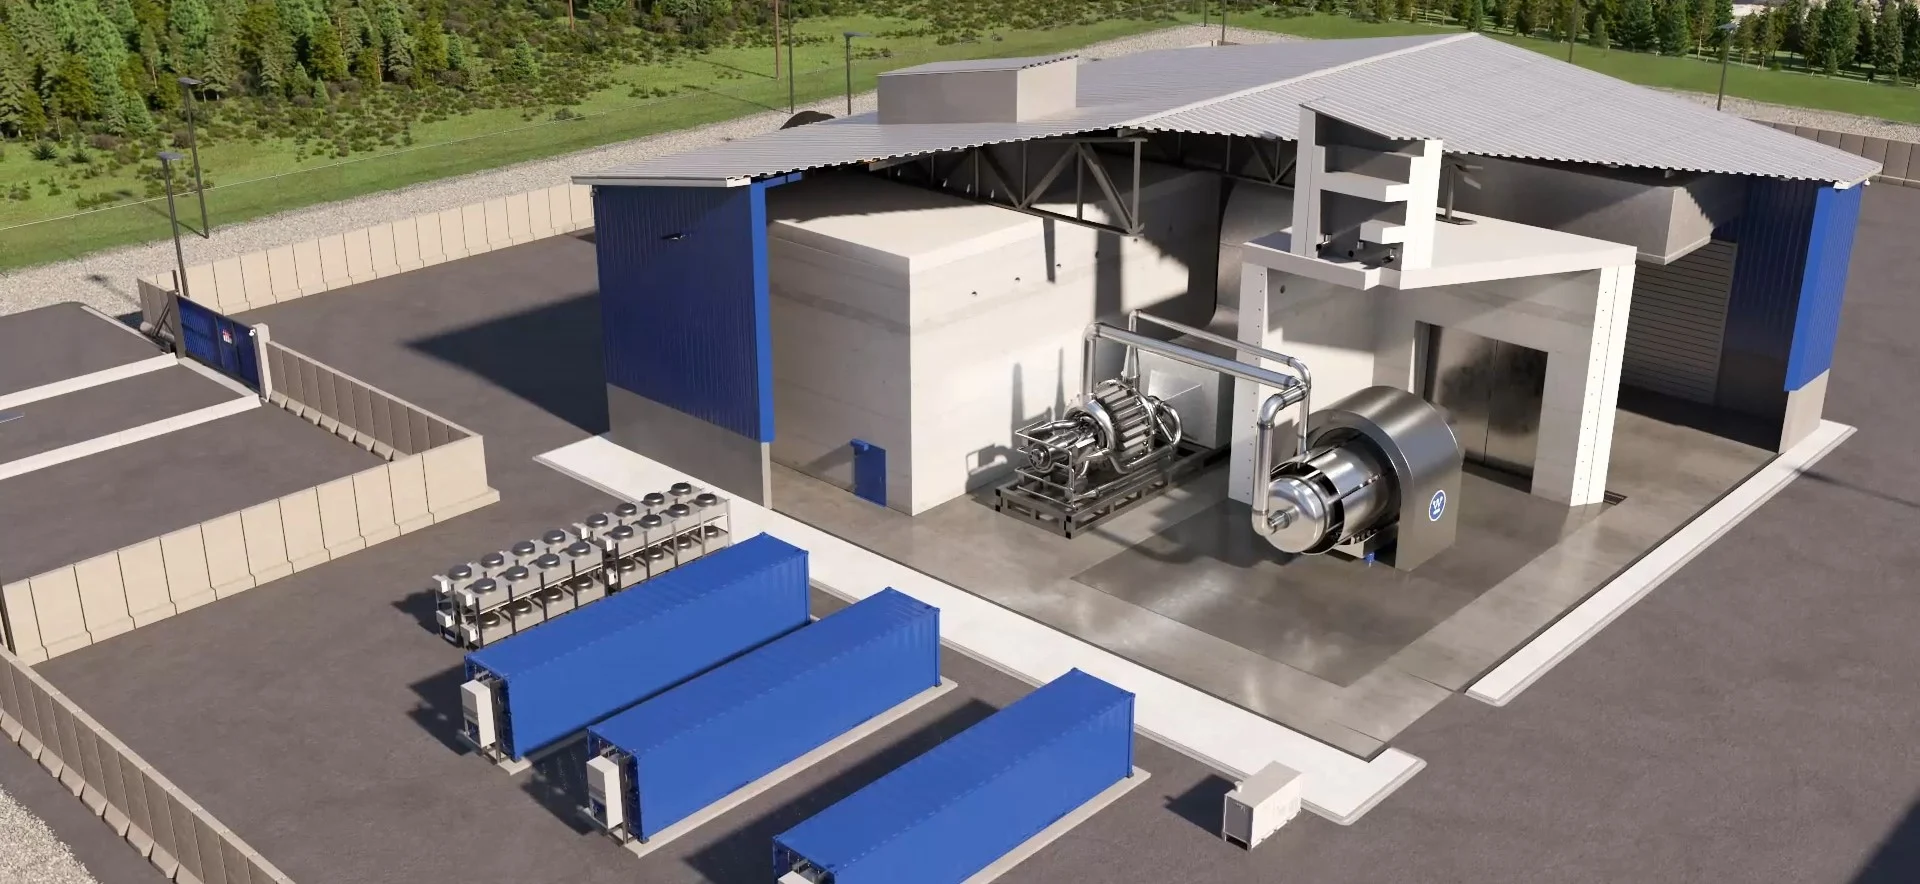
\includegraphics[width=0.7\textwidth]{content/figures/evinci.jpg}
    \caption{Render del \emph{eVinci$^{TM}$ Microreactor} de Westinghouse, con una potencia de 5 MWe y 13 MWt (\cite{evinci}).}
    \label{fig:evinci}
\end{figure}

\begin{table}[]
  \resizebox{\textwidth}{!}{%
  \begin{tabular}{|
  >{\columncolor[HTML]{FFCCC9}}c |c|c|c|c|c|}
  \hline
  \cellcolor[HTML]{ECF4FF}\textbf{Diseño} &
    \cellcolor[HTML]{ECF4FF}\textbf{Potencia (MWe)} &
    \cellcolor[HTML]{ECF4FF}\textbf{Tipo} &
    \cellcolor[HTML]{ECF4FF}\textbf{Diseñador} &
    \cellcolor[HTML]{ECF4FF}\textbf{País} &
    \cellcolor[HTML]{ECF4FF}\textbf{Estado} \\ \hline
  Energy Well & 8        & \acrshort{fhr} & Centrum výzkumu Řež & República Checa & Diseño pre-conceptual \\ \hline
  MoveluX &
    3 – 4 &
    \begin{tabular}[c]{@{}c@{}}Tubos de disipación\\ de calor (\acrshort{hpr})\end{tabular} &
    \begin{tabular}[c]{@{}c@{}}Toshiba Energy\\ Systems \& Solutions\\ Corporation\end{tabular} &
    Japón &
    Diseño conceptual \\ \hline
  ELENA &
    0,068 &
    \acrshort{pwr} &
    \begin{tabular}[c]{@{}c@{}}National Research\\ Centre\\ “Kurchatov Institute”\end{tabular} &
    Rusia &
    Diseño conceptual \\ \hline
  UNITHERM    & 6,6      & \acrshort{pwr}  & NIKIET              & Rusia           & Diseño conceptual     \\ \hline
  AMR         & 3        & \acrshort{htgr} & STL Nuclear (Pty)   & Sudáfrica       & Diseño pre-conceptual \\ \hline
  LFR-TL-30   & 30       & \acrshort{lmfr} & newcleo             & Reino Unido     & Diseño conceptual     \\ \hline
  U-Battery   & 4        & \acrshort{htgr} & Urenco              & Reino Unido     & Diseño conceptual     \\ \hline
  Aurora      & 1,5 – 50 & \acrshort{lmfr} & OKLO                & EEUU            & Diseño detallado      \\ \hline
  HOLOS-QUAD  & 10       & \acrshort{htgr} & HolosGen LLC        & EEUU            & Diseño detallado      \\ \hline
  MARVEL &
    0,015 – 0,027 &
    \acrshort{lmfr} &
    \begin{tabular}[c]{@{}c@{}}Idaho National\\ Laboratory\end{tabular} &
    EEUU &
    \begin{tabular}[c]{@{}c@{}}Fabricación de equipos\\ en proceso\end{tabular} \\ \hline
  MMR$^{TM}$ &
    \textgreater 5 y \textgreater 10 &
    \acrshort{htgr} &
    \begin{tabular}[c]{@{}c@{}}Ultra Safe Nuclear\\ Corporation\end{tabular} &
    EEUU &
    Diseño básico \\ \hline
  \begin{tabular}[c]{@{}c@{}}Westinghouse\\ eVinci$^{TM}$\end{tabular} &
    2 – 3,5 &
    \begin{tabular}[c]{@{}c@{}}Tubos de disipación\\ de calor (\acrshort{hpr})\end{tabular} &
    Westinghouse &
    EEUU &
    \begin{tabular}[c]{@{}c@{}}Diseño conceptual\\ completado\end{tabular} \\ \hline
  \end{tabular}%
  }
  \caption{Diseños existentes de MMRs (\cite{iaea_smr_booklet_2022}).}
  \label{tab:mmrs}
  \end{table}

\subsection{AP300 Small Modular Reactor}

A continuación, se pretende estudiar con detalle el diseño, las características y el funcionamiento del AP300, que se ha escogido debido a su avanzado grado de desarrollo, su previsión de despliegue a corto plazo y su parecido con la Central Nuclear José Cabrera ---véase el apartado \ref{comparacion_zorita_ap300}---, cuyo simulador interactivo se emplea en el presente proyecto.

\subsubsection{Introducción y contextualización}

El AP300 es un proyecto de \acrshort{smr} de 300 MWe que presentó Westinghouse en mayo de 2023, consistente en una versión a menor escala del reactor de Generación III+ AP1000. Este último, es un diseño de reactor avanzado de 1.110 MWe del que hoy en día existen 6 unidades en operación: 4 en China y 2 en EEUU. Además, múltiples reactores nucleares actulamente en construcción en el mundo son de este tipo, y existen contratos de despliegue de esta tecnología en varios países, como es el caso de Ucrania, China, EEUU, Polonia, Bulgaria, India y Países Bajos.

Una característica fundamental de este pequeño reactor modular es que, a diferencia de los demás \acrshortpl{smr} en desarrollo ---con las nuevas tecnologías y riesgos derivados de un nuevo tipo de reactor---, el AP300 utiliza la ingeniería, los componentes y la cadena de suministro del AP1000, confiriendo al nuevo proyecto una gran ventaja práctica. 

De esta manera, se prevee que se aprueben las licencias de operación para 2027 y que se conecte a la red en 2033. El período de construcción estimado es de unos 3 años y el coste del mismo es de 1.000 millones de euros por unidad ---coste unitario estimado de unos 3.400 \$/kWe--- (\cite{ap300_westinghouse}).

\begin{figure}[h]
  \centering
  \includegraphics[width=0.7\textwidth]{content/figures/ap300.png}
  \caption{Render del AP300 (\cite{ap300_westinghouse}).}
  \label{fig:AP300}
\end{figure}

Cabe mencionar que, en febrero de 2024, Westinghouse firmó un acuerdó con \emph{Community Nuclear Power} ---una empresa de desarrollo de \acrshortpl{smr} de Reino Unido--- para construir cuatro \acrshortpl{smr} AP300 en la región \emph{North Teesside}, al noreste de Inglaterra, con el fin de que comiencen a operar a principios de la década de 2030 (\cite{uk_ap300_deployment}).

\subsubsection{Características comunes con el AP1000}

El AP300 es un \acrshort{smr} de agua a presión (\acrshort{pwr}) de un solo lazo, con una potencia eléctrica de 300 MWe y una potencia térmica de 990 MWt. Tal y como se ha comentado anteriormente, utiliza la misma tecnología y procedimientos que el reactor AP1000 en los siguientes aspectos: 

\begin{itemize}
  \item Metodologías de diseño y licenciamiento.
  \item Técnicas de construcción. Por ejemplo, cimientos del edificio análogos a los del AP1000 o vasija del reactor forjada en anillo en vez de emplear soldaduras longitudinales.
  \item Procedimientos de operación y mantenimiento.
  \item Equipos y componentes principales. Por ejemplo, el empleo de presurizadores más grandes aumenta los márgenes de operación transitorio, aumentando así la seguridad.
  \item Tecnología de instrumentación y control.
  \item Sistemas de seguridad pasiva.
  \item Combustible: uranio de bajo enriquecimiento (\acrshort{leu}).
  \item Cadena de suministro. La mayor parte del equipamiento procederá de los proveedores escogidos para el AP1000.
  \item Módulos estructurales compuestos de acero y hormigón.
  \item Módulos prefabricados de salas de la planta con sus respectivos equipos.
  \item Capacidad avanzada de seguimiento de carga sin necesidad de productos químicos (con tasas de rampa de $\pm5\%/min$ hasta alcanzar el 15\% de la potencia total, en el caso del AP1000).
\end{itemize}
Uno de los principales objetivos de diseño del AP1000, que también comparte el AP300, es la \textbf{simplificación} en los sistemas de seguridad, en los sistemas de operación normal, en la sala de control, en las técnicas de construcción y en los sistemas de instrumentación y control. El motor principal de este objetivo es proporcionar una tecnología que es más fácil y menos costosa de construir, operar y mantener. El resultado de esta simplificación es una considerable reducción en la cantidad de válvulas, bombas, cables, material de construccion y otros componentes, todos los cuales contribuyen a un ahorro considerable en la inversión de capital y a costos más bajos de operación y mantenimiento. Todo esto optimizado sin reducir ---más bien aumentando--- el nivel de seguridad incorporada.

En lo que se refiere a la \textbf{seguridad}, el AP300 se basa en los avanzados sistemas empleados en los AP1000, distinguiendo 3 principales tipos de sistemas de seguridad:

\begin{itemize}
  \item \underline{Sistemas activos de defensa en profundidad:} Son múltiples sistemas adicionales que, sin ser estrictamente necesarios para mitigar accidentes de base de diseño\footnote{Accidentes graves que se postula que pueden ocurrir en una instalación nuclear y que sirven de base para el diseño de sus sistemas de protección.}, se encargan de \textbf{respaldar la operación normal de la planta} y servir de primera línea de defensa en caso de transitorios o contratiempos, en los cuales se pondrían automáticamente en funcionamiento los sistemas pasivos de seguridad. 
  
  Aunque estos sistemas no se contemplan en la evaluación del análisis de seguridad, proporcionan una defensa en profundidad adicional al agregar una capa de redundancia y diversidad. Cabe mencionar que estos sistemas requieren menos inspecciones, pruebas y mantenimiento que los principales sistemas de seguridad ---los pasivos---. Algunos ejemplos de este tipo de sistemas son los siguientes:

  \begin{itemize}
    \item Sistema de control químico y volumétrico (del inglés, \acrshort{cvcs}).
    \item Sistema normal ---no pasivo--- de extracción de calor residual (del inglés, \acrshort{rhrs}).
    \item Sistema de alimentación de agua de arranque (auxiliar).
    \item Sistema de control de hidrógeno de la contención (consta del sistema de monitoreo de hidrógeno).
    \item R\gls{ecombinadores pasivos} autocatalíticos de hidrógeno\footnote{Eliminan los posibles gases combustibles generados dentro de la contención en accidentes severos mediante la recombinación o combustión de una manera gradual, minimizando así el riesgo de una explosión de hidrógeno.}.
    \item Encendedores de hidrógeno\footnote{Eliminan el hidrógen del edificio de contención mediante el quemado del mismo por un encendedor eléctrico.} alimentados por baterías.
    \item Sistemas de calefacción, ventilación y aire acondicionado (del inglés, \acrshort{hvac}), que eliminan el calor de las salas de instrumentación y control, y de la sala de control principal.
  \end{itemize}

Estos sistemas utilizan sistemas de soporte como los generadores diésel de reserva, el sistema de enfriamiento de componentes y el sistema de agua de servicio. 
  
  \item \underline{Sistemas pasivos de seguridad:} Consisten ---tal y como se ha detallado en el apartado \ref{seguridad}--- en aquellos sistemas cuya actuación se asegura por principios físicos ---como la gravedad, la circulación natural de fluidos o el empleo de gases comprimidos--- independientes de energía externa, sin requerir la acción de un operador o de realimentación electrónica.
  En el AP300 estos son los \textbf{principales sistemas de seguridad} que, de forma autónoma e independiente, responden frente a cualquier accidente base de diseño, estableciendo y manteniendo automáticamente la refrigeración del núcleo, y asegurando la integridad del confinamiento por tiempo indefinido. No se emplean bombas, ventiladores, generadores diésel, enfriadores u otro tipo de maquinaria activa, tan solo unas válvulas que se alinean automáticamente y accionan los sistemas de seguridad pasivos.
  Adicionalmente, existen sistemas pasivos redundantes de mitigación de accidentes, diseñados para responder correctamente ante la peor consecución de sucesos en caso de accidente.
  
  Algunos de estos sistemas son:
  \begin{itemize}
    \item Sistema de refrigeración pasiva del núcleo.
    \item Sistema de enfriamiento pasivo de la contención (del inglés, \acrshort{pcs}).
    \item Sistema de habitabilidad de emergencia de la sala de control principal.
    \item Inyección de seguridad a alta presión con tanques de recarga del núcleo.
    \item Inyección de seguridad a media presión con acumuladores.
    \item Recarga del refrigerante del reactor a baja presión desde el tanque de almacenamiento de agua de recarga (del inglés, \acrshort{rwst}).
    \item Sistema pasivo de extracción del calor residual (del inglés, \acrshort{prhrs}).
    \item Sistema de depresurización automática.
  \end{itemize}
  
  Cabe destacar la capacidad de estos sistemas de seguridad pasiva de afrontar de forma segura más de 72 horas después de un apagón en la planta.

  \begin{figure}[h]
    \centering
    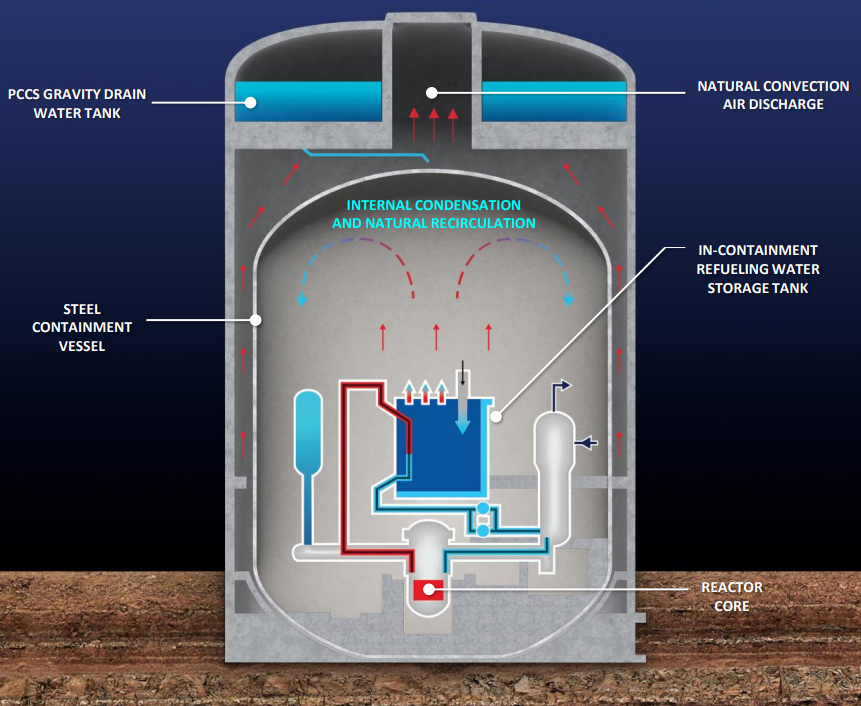
\includegraphics[width=0.7\textwidth]{content/figures/ap300_safety_systems.png}
    \caption{Esquema con las principales partes y sistemas de seguridad del edificio de contención del AP300 (\cite{ap300_westinghouse}).}
    \label{fig:ap300_safety_systems}
  \end{figure}

  \item \underline{Sistemas de mitigación de accidentes severos:} Son aquellos sistemas que, ante un accidente severo en la central, retienen los productos de fisión dentro de la vasija, proporcionan medios seguros de refrigeración de núcleo dañado y previenen la interacción del núcleo fundido con el hormigón, lo que podría ocasionar la liberación de material radioactivo al medio ambiente.
  
  El reactor AP300 está diseñado para drenar el agua del tanque de almacenamiento de agua de recarga de alta capacidad (\acrshort{rwst}) dentro del confinamiento hacia la cavidad del reactor en caso de sobrecalentamiento del núcleo. Esto proporciona enfriamiento en el exterior del recipiente del reactor, previendo así el fallo del recipiente del reactor y el posterior derrame de escombros del núcleo fundido en el confinamiento.
\end{itemize}

A parte de estos sistemas pasivos ---y activos de apoyo---, el reactor AP300 incorpora las necesarias barreras físicas que aseguran el confinamiento de los materiales radiactivos: las pastillas y vainas de combustible, la vasija del reactor, la vasija de contención de acero y el edificio de contención de hormigón armado. Estas dos últimas barreras físicas ofrecen una robusta protección ante daños extremos procedentes del exterior del reactor, desde catástrofes naturales de elevada intensidad a impactos de aviones a grandes velocidades.

Todos estos sistemas de seguridad ya fueron extensamente analizados y comprobados para el desarrollo del AP1000, siendo asimismo revisados y aprobados por los correspondientes reguladores de seguridad.


\subsubsection{Diferencias con el AP1000}

A parte de las evidentes diferencias de escala y tamaño por la menor potencia del pequeño reactor modular ---los edificios relacionados con la seguridad del reactor ocupan tan solo 1.600 $m^2$ aproximadamente---, cabe destacar las siguientes características del AP300 que lo distinguen del AP1000:

\begin{itemize}
  \item Mientras que el AP1000 es un reactor de dos lazos, el AP300 es ---como ya se ha comentado--- de un solo lazo. Se reducen así el número de soportes y soldaduras necesarias, así como la cantidad de material necesaria.
  \item Se ha concebido con una vida de diseño de más de 80 años, en comparación con la vida de diseño de 60 años del AP1000. 
  \item Se esperan ciclos de operación de 4 años (con previbles extensiones en el futuro), frente a los ciclos de 1 año y medio de su predecesor.
  \item Los elementos de combustible son de $12 \times  12$ varillas, en vez de la disposición de $17 \times 17$ del AP1000.
  \item El generador de vapor que emplea es el Delta 76, más pequeño que los empleados en el AP1000 (Delta 125).
  \item Se emplean pastillas de combustible dopadas con óxido crómico ($C_3O_2$) y alúmina ($Al_2O_3$) para mejorar las propiedades y la economía del ciclo de combustible.
  \item El diseño ``ultra compacto'' ---tal y como lo define la propia empresa--- reduce, a parte del tamaño global de la planta, la extensión de paredes y suelos, con una consecuente reducción en la cantidad de material necesario.
  \item El punto anterior conlleva una consecuente reducción de costes y tiempos de construcción, tal y como se muestra en la siguiente tabla, en la que se especifican los datos reales del AP1000 y los datos estimados del AP300:
\end{itemize}

\begin{table}[h]
  \centering
  \resizebox{0.9\textwidth}{!}{%
  \begin{tabular}{c|c|c|c|c|c|}
    \cline{2-6}
     &
      \cellcolor[HTML]{ECF4FF}\begin{tabular}[c]{@{}c@{}}Potencia\\ eléctrica\\ (MWe)\end{tabular} &
      \cellcolor[HTML]{ECF4FF}\begin{tabular}[c]{@{}c@{}}Potencia\\ térmica\\ (MWt)\end{tabular} &
      \cellcolor[HTML]{ECF4FF}\begin{tabular}[c]{@{}c@{}}Tiempo de\\ construcción\\ (años)\end{tabular} &
      \cellcolor[HTML]{ECF4FF}\begin{tabular}[c]{@{}c@{}}Coste de\\ construcción\\ (\$)\end{tabular} &
      \cellcolor[HTML]{ECF4FF}\begin{tabular}[c]{@{}c@{}}Coste por unidad\\ de potencia instalada\\ (\$/kWe)\end{tabular} \\ \hline
    \multicolumn{1}{|c|}{\cellcolor[HTML]{FFCCC9}AP1000} &
      1.110 &
      3.415 &
      9 &
      15.170.000.000 &
      13.666,67 \\ \hline
    \multicolumn{1}{|c|}{\cellcolor[HTML]{FFCCC9}AP300} &
      300 &
      990 &
      3 &
      1.000.000.000 &
      3.400 \\ \hline
    \end{tabular}
  }
  \caption{Comparación en potencia, tiempo y coste entre el AP1000 ---del cual se aportan los datos históricos reales de la construcción de la unidad Vogtle-3 en EEUU--- y el AP300 ---del cual se aportan los valores estimados por Westinghouse--- (\cite{vogtle_costs,construction_schedules})}
  \label{tab:ap1000_vs_ap300}
  \end{table}

\begin{figure}[h]
  \centering
  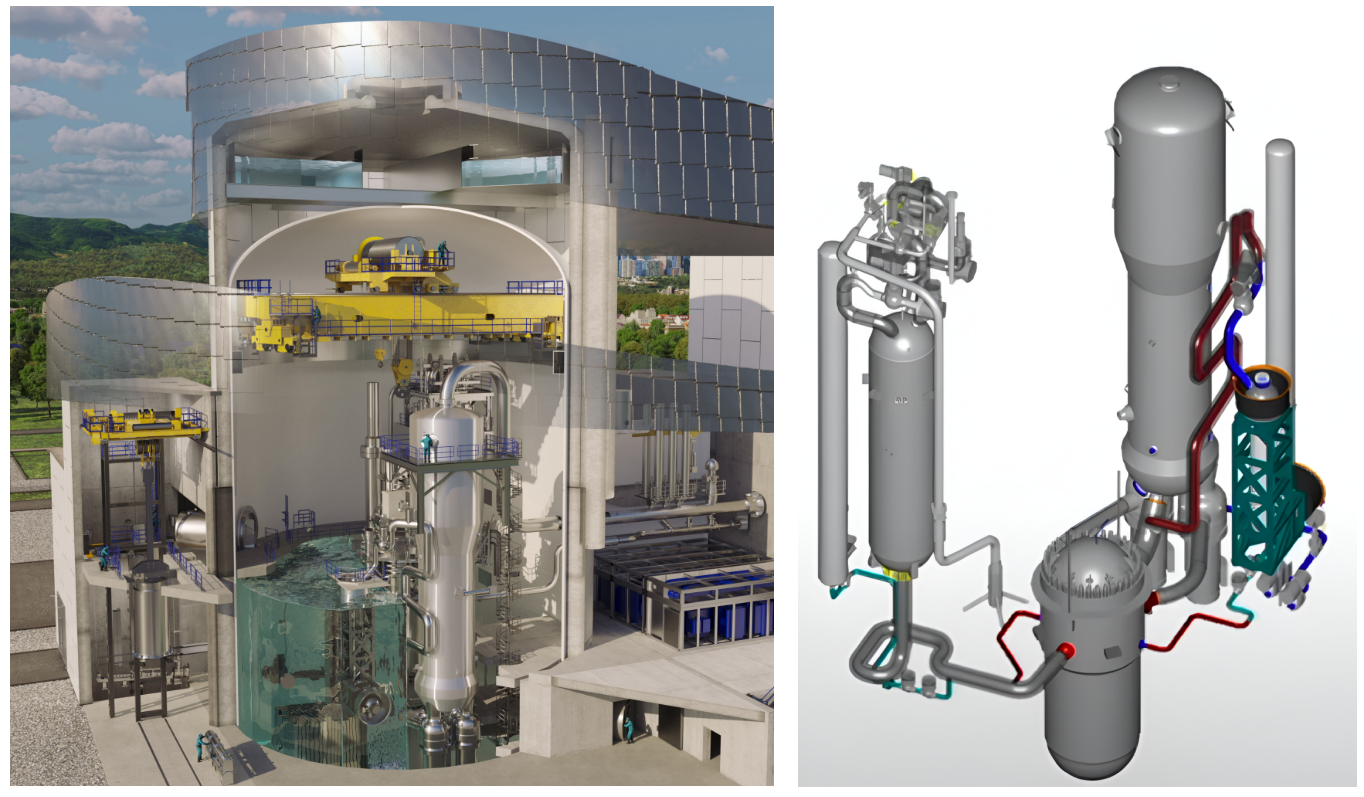
\includegraphics[width=\textwidth]{content/figures/ap300_inside_nsss.png}
  \caption{Render del interior del edificio principal de la planta ---a la izquierda--- y detalle 3D del \acrshort{nsss} del AP300 ---a la derecha--- (\cite{ap300_westinghouse}).}
  \label{fig:ap300_inside_nsss}
\end{figure}

 Por último, en lo que se refiere a sus \textbf{aplicaciones}, se espera que, a parte de ofrecer electricidad de forma confiable, segura y limpia, el AP300 se emplee para la calefacción urbana y la desalinización de agua. Además, sus capacidades de seguimiento de carga rápida lo hacen ideal para la integración con fuentes de energía renovables. Asimismo, allanará el camino hacia la economía del hidrógeno al permitir la producción de hidrógeno integrada con la planta (véase el apartado \ref{cogeneracion} para obtener información detallada sobre la desalación, la producción de hidrógeno y otras aplicaciones no eléctricas de los \acrshortpl{smr}).

 \begin{figure}[h]
  \centering
  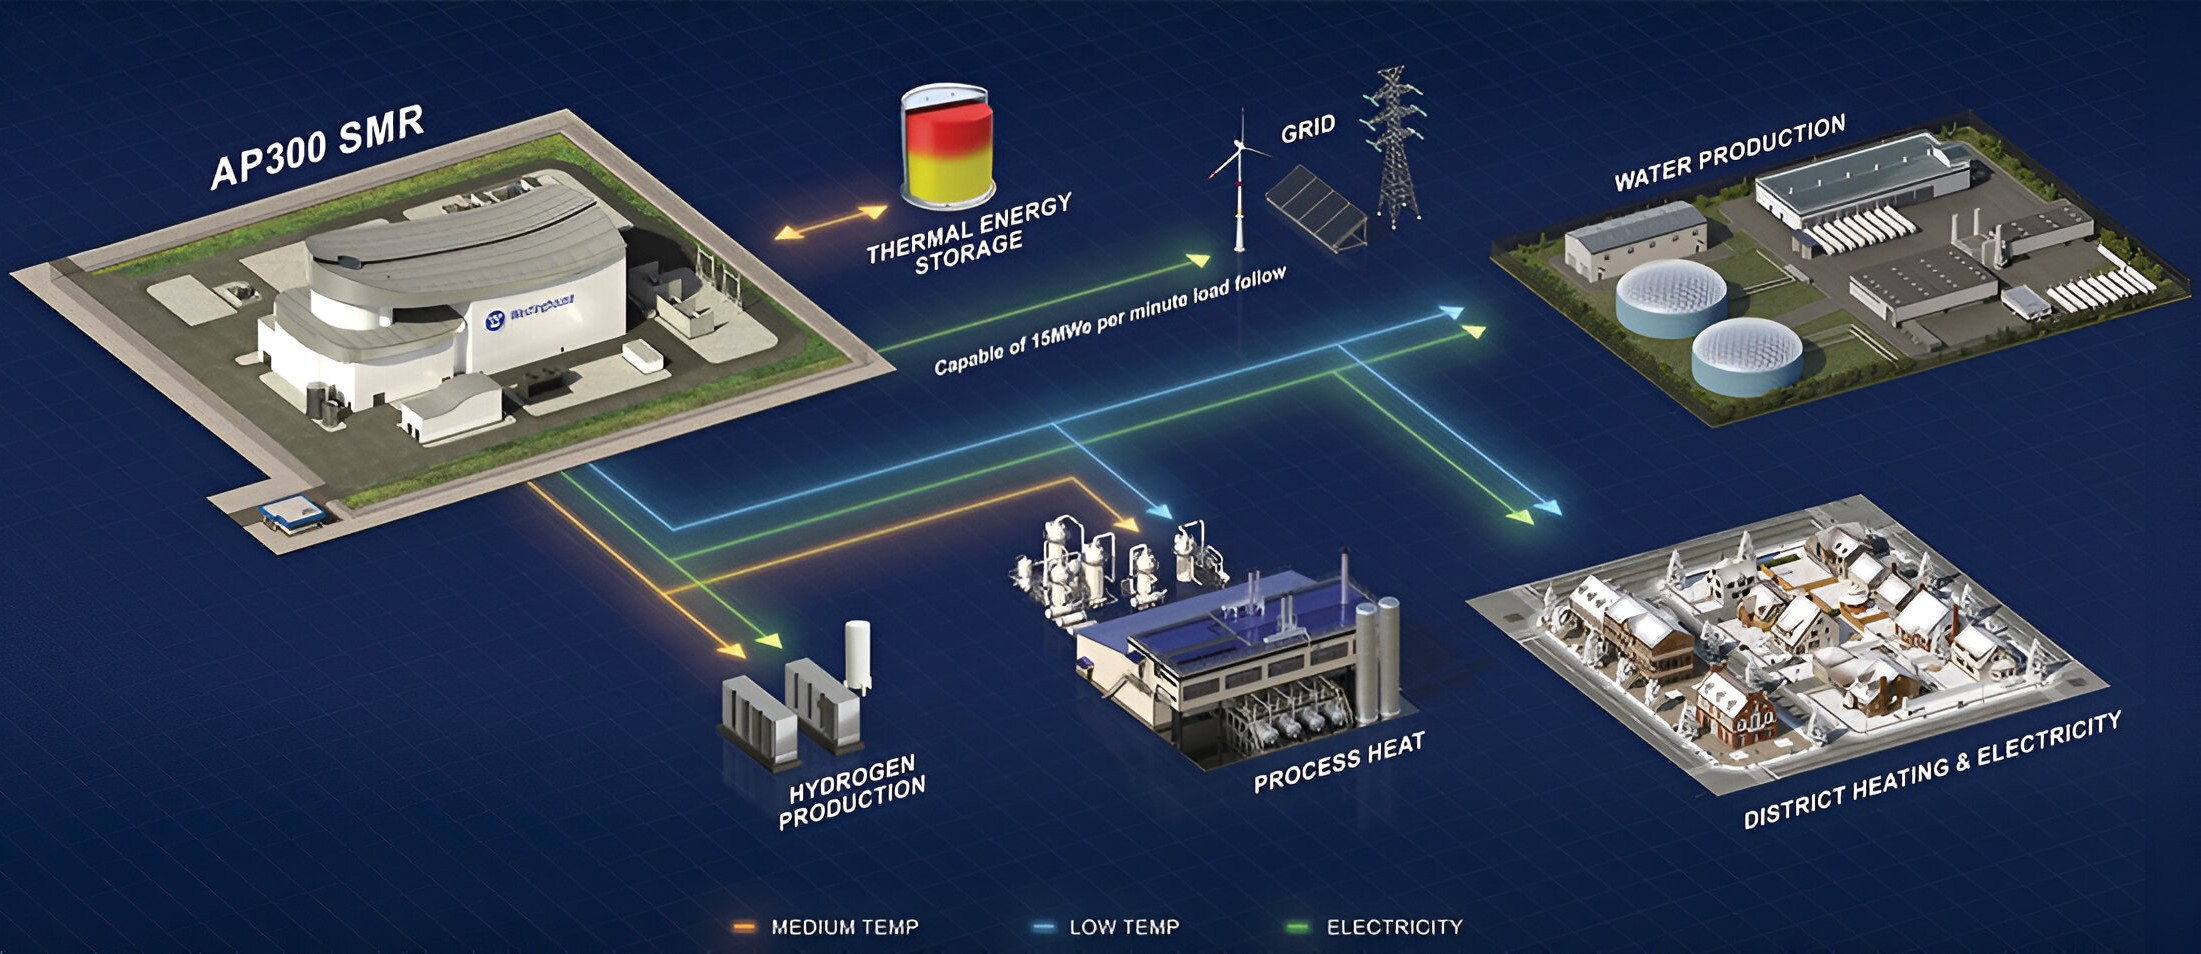
\includegraphics[width=\textwidth]{content/figures/ap300_applications.jpeg}
  \caption{Diversidad de aplicaciones del AP300 (\cite{ap300_westinghouse}).}
  \label{fig:AP300_applications}
\end{figure}

\newpage

% Formato APA (el recomendado para TFG)

\appto{\bibsetup}{\sloppy}

\printbibliography[heading=bibintoc, title=BIBLIOGRAFÍA] % Aparecen únicamente las referencias citadas a lo largo del documento
%%%%%%%%%%%%%%%%%%% - ANEXOS - %%%%%%%%%%%%%%%%%%%

\newpage
\section*{ANEXOS} \label{sec:anexos} % Se añade un asterisco a \section para que el título no esté numerado.
\phantomsection
\addcontentsline{toc}{section}{ANEXOS} % Al utilizar \section* se ha de añadir manualmente el apartado al índice (Table Of Contents, TOC).
\markright{ANEXOS} % Al utilizar \section* se ha de añadir manualmente el título del apartado al encabezado.

\renewcommand{\thesubsection}{\Alph{subsection}} % Se numeran los anexos con letras del alfabeto en lugar de números.
% Se indica que las tablas, figuras y códigos se numeran con el código del anexo (A, B, C, ...) seguido del número de tabla, figura o código dentro del anexo (tabla A.2, figura C.1, etc.)
\renewcommand{\thetable}{\Alph{subsection}.\arabic{table}}
\renewcommand{\thefigure}{\Alph{subsection}.\arabic{figure}}
\renewcommand{\thecode}{\Alph{subsection}.\arabic{code}}

% ---------------- Primer anexo ---------------- %
\setcounter{subsection}{0}
\setcounter{table}{0}
\setcounter{figure}{0}

\subsection{Gráficas obtenidas en la segunda simulación larga fallida} \label{graficas_erroneas}

\textit{Simulación de 6 horas y 40 minutos realizada en el \acrshort{sgiz} el 30 de abril de 2024.}

A continuación, se muestran algunas de las gráficas obtenidas en la simulación fallida explicada en el apartado \ref{sim_larga_fallida}, con una estabilización incorrecta a partir de las 4 horas:

\begin{figure}[!h]
    \centering
    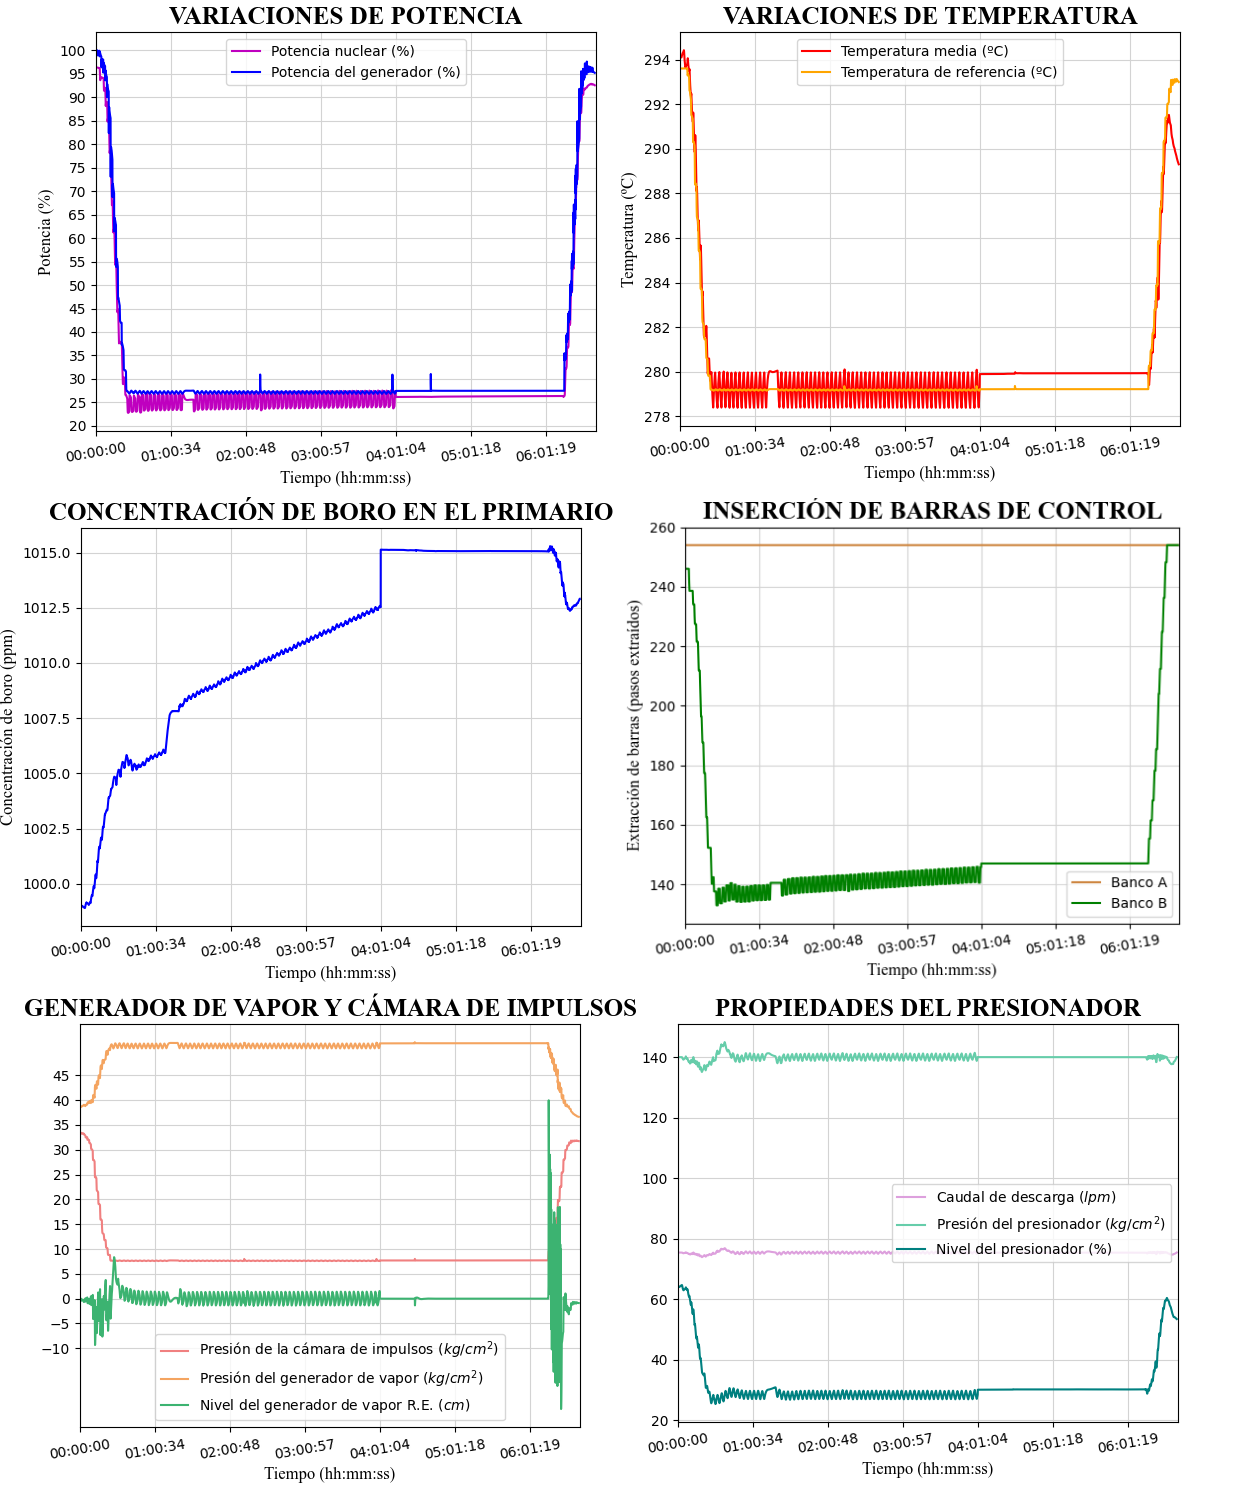
\includegraphics[width=\textwidth]{content/figures/sim2_peque.png}
    \caption{Gráficas imperfectas de la segunda simulación larga fallida.}
    \label{fig:sim2_peque}
\end{figure}

\newpage
\subsection{Resultados de la encuesta de la práctica} \label{resultados_encuesta_practica}

Tal y como se comenta en el apartado \ref{feedback_practica}, tras la realización de la práctica de seguimiento de carga en el \acrshort{sgiz} por parte de 28 alumnos de la asignatura de \textit{Tecnologías Avanzadas en Reactores Nucleares} del máster, se envió una encuesta para obtener retroalimentación sobre la sesión. A continuación, se muestran los resultados detallados de las 12 respuestas obtenidas:

\begin{enumerate}
    \item \textbf{¿Habías hecho alguna práctica similar en el \acrshort{sgiz} anteriormente?}
    
    \begin{figure}[!h]
        \centering
        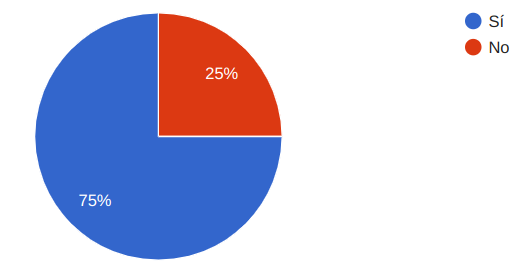
\includegraphics[width=0.47\textwidth]{content/figures/encuesta_1.png}
        \caption{Resultados pregunta 1.}
        \label{fig:encuesta_1}
    \end{figure}

    \item \textbf{¿Crees que la práctica se enmarca adecuadamente en la asignatura de Tecnologías Avanzadas en Reactores Nucleares?}
    
    \begin{figure}[!h]
        \centering
        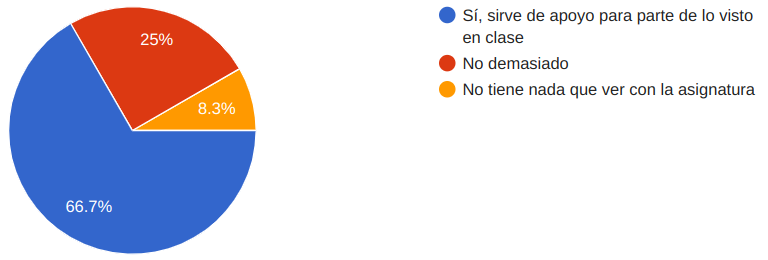
\includegraphics[width=0.72\textwidth]{content/figures/encuesta_2.png}
        \caption{Resultados pregunta 2.}
        \label{fig:encuesta_2}
    \end{figure}
    
    \item \textbf{¿Habías oído hablar antes de las capacidades avanzadas de seguimiento de carga para las que se diseñan los \acrlongpl{smr}?}
    
    \begin{figure}[!h]
        \centering
        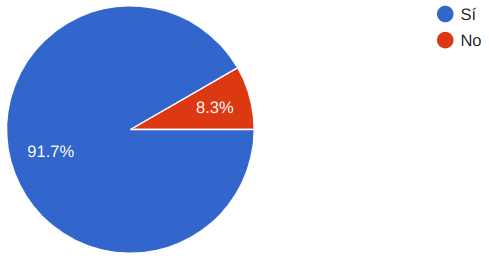
\includegraphics[width=0.47\textwidth]{content/figures/encuesta_3.png}
        \caption{Resultados pregunta 3.}
        \label{fig:encuesta_3}
    \end{figure}
    
    \newpage
    \item \textbf{¿Has aprendido cosas nuevas con la práctica?}
    \newline
    \begin{figure}[h]
        \centering
        \vspace{-0.5cm}
        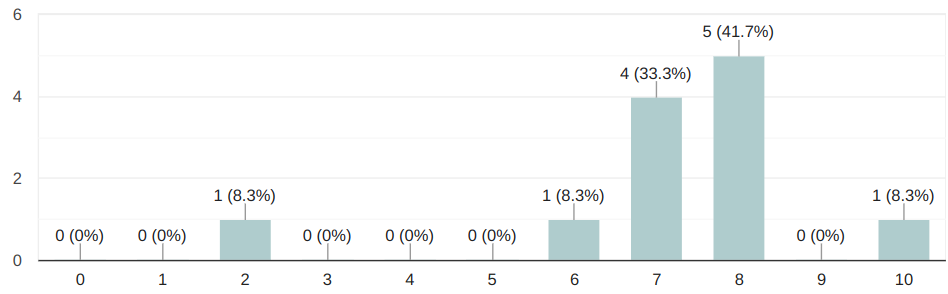
\includegraphics[width=\textwidth]{content/figures/encuesta_4.png}
        \caption{Resultados pregunta 4.}
        \label{fig:encuesta_4}
    \end{figure}
    
    \item \textbf{¿Te ha ayudado a comprender mejor las características y el funcionamiento general de los principales componentes y sistemas del reactor durante la operación del mismo?}
    
    \begin{figure}[h]
        \centering
        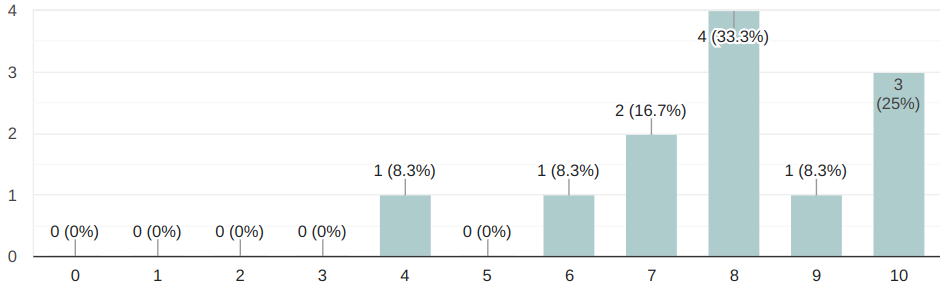
\includegraphics[width=\textwidth]{content/figures/encuesta_5.png}
        \caption{Resultados pregunta 5.}
        \label{fig:encuesta_5}
    \end{figure}
    
    \item \textbf{¿Se han entendido bien el objetivo, el procedimiento y las conclusiones de la simulación realizada? ¿Las explicaciones han sido suficientemente claras?}
    
    \begin{figure}[!h]
        \centering
        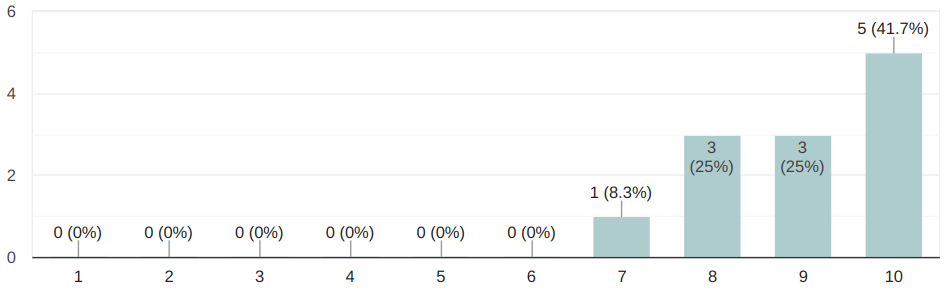
\includegraphics[width=\textwidth]{content/figures/encuesta_6.png}
        \caption{Resultados pregunta 6.}
        \label{fig:encuesta_6}
    \end{figure}
    
    \newpage
    \item \textbf{En general, ¿crees que realizar prácticas en el simulador ayuda a entender mejor lo visto en algunas asignaturas del grado y del máster?}
    
    \begin{figure}[!h]
        \centering
        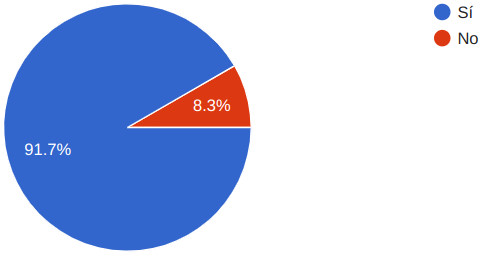
\includegraphics[width=0.47\textwidth]{content/figures/encuesta_7.png}
        \caption{Resultados pregunta 7.}
        \label{fig:encuesta_7}
    \end{figure}

    \item \textbf{Finalmente, valora del 0 al 10 tu grado de satisfacción general con la práctica realizada:}
    
    \begin{figure}[!h]
        \centering
        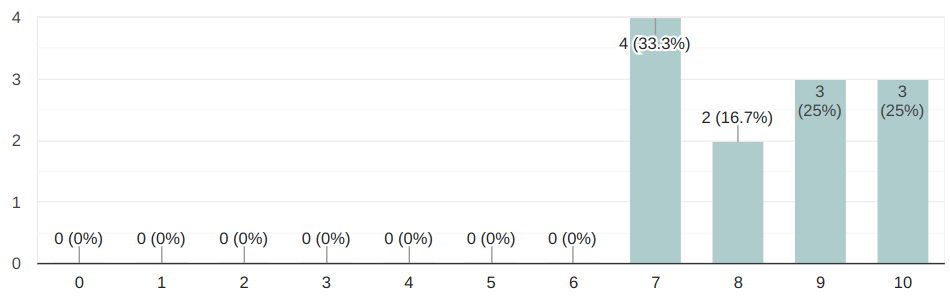
\includegraphics[width=\textwidth]{content/figures/encuesta_8.png}
        \caption{Resultados pregunta 8.}
        \label{fig:encuesta_8}
    \end{figure}
\end{enumerate}

Además de las 8 preguntas mostradas, se añadió una sección en el formulario para que los alumnos hicieran comentarios adicionales. La información aportada en esa sección es de gran utilidad y se encuentra resumida en el apartado \ref{feedback_practica}.

\newpage
\subsection{Código} \label{sec:codigo}

Todas las gráficas de las simulaciones realizadas en el \acrshort{sgiz} han sido elaboradas con \textit{Python} a partir de los datos generados en \textit{Excel} por el propio simulador. A continuación, se muestra, a modo de ejemplo, el código para la obtención de una de las gráficas:

\vspace{-5pt}

\begin{code}[H]
\begin{lstlisting}[firstnumber=1, breakindent=55pt]
  # Importación de las librerías necesarias
  import matplotlib.pyplot as plt
  import numpy as np
  import pandas as pd

  # Obtención de datos:
  gen_vapor_camara_imp=pd.read_excel("simulacion3.xlsx","gen_vapor_camara_imp")
  df_gen_vapor_camara_imp=pd.DataFrame=gen_vapor_camara_imp

  tiempo=[]
  for i in range(0,len(df_gen_vapor_camara_imp.tiempo)):
      tiempo.append(df_gen_vapor_camara_imp.tiempo[i].strftime('%H:%M:%S'))
    
  pres_cam_imp=[]
  for i in range(0,len(df_gen_vapor_camara_imp.pres_cam_imp)):
      pres_cam_imp.append(df_gen_vapor_camara_imp.pres_cam_imp[i])

  presion_gen_vapor=[]
  for i in range(0,len(df_gen_vapor_camara_imp.               presion_gen_vapor)):
      presion_gen_vapor.append(df_gen_vapor_camara_imp.presion_gen_vapor[i])

  nivel_gen_vapor=[]
  for i in range(0,len(df_gen_vapor_camara_imp.nivel_gen_vapor)):
      nivel_gen_vapor.append(df_gen_vapor_camara_imp.nivel_gen_vapor[i])

  # Creación del gráfico
  plt.plot(tiempo, presion_camara_impulsos, label='Presión de la cámara de impulsos $(kg/cm^2)$', color='lightcoral')
  plt.plot(tiempo, presion_gen_vapor, label='Presión del generador de vapor $(kg/cm^2)$', color='sandybrown')
  plt.plot(tiempo, nivel_gen_vapor, label='Nivel del generador de vapor R.E. $(cm)$', color='mediumseagreen')

  # Creación de la leyenda y el título
  plt.legend(loc='best')
  plt.xlabel('Tiempo (hh:mm:ss)', family='Times New Roman', size=12)
  plt.title('COMPORTAMIENTO GENERADOR DE VAPOR Y CÁMARA DE IMPULSOS', fontname='Times New Roman', size=18, weight='bold')
  plt.grid(True, color='lightgrey')
  plt.yticks(np.arange(-10,50,5))
  plt.xlim([0, len(tiempo)])
  plt.xticks(np.arange(0,len(tiempo),360))
  plt.xticks(rotation = 10)

  # Mostrar el gráfico
  plt.show()
\end{lstlisting}
\vspace{-5pt}
\caption{Ejemplo del código utilizado para generar las gráficas de las simulaciones. Este en concreto corresponde al código de la figura \ref{fig:sim3_gen_vapor_camara_imp}.}
\label{cod:codigo_graficas}
\end{code}

%%%%%%%%%%%%%% - ÍNDICE DE TABLAS - %%%%%%%%%%%%%%
\newpage
\renewcommand{\listtablename}{ÍNDICE DE TABLAS} % Se define el nombre del índice de tablas.
\listoftables % Se genera automáticamente el índice con las distintas tablas del documento (entorno \table o \longtable).
\addcontentsline{toc}{section}{ÍNDICE DE TABLAS} % Se añade manualmente el apartado al índice (Table Of Contents, TOC).


%%%%%%%%%%%%% - ÍNDICE DE FIGURAS - %%%%%%%%%%%%%%
\newpage
\renewcommand{\listfigurename}{ÍNDICE DE FIGURAS} % Se define el nombre del índice de figuras.
\listoffigures % Se genera automáticamente el índice con las distintas figuras del documento (entorno \figure).
\addcontentsline{toc}{section}{ÍNDICE DE FIGURAS} % Se añade manualmente el apartado al índice (Table Of Contents, TOC).

%%%%%%%%%%%%% - ABREVIATURAS, UNIDADES Y ACRÓNIMOS - %%%%%%%%%%%%%%
\newpage
\printnoidxglossary[title={ABREVIATURAS, UNIDADES Y ACRÓNIMOS}]
\addcontentsline{toc}{section}{ABREVIATURAS, UNIDADES Y ACRÓNIMOS}
\newpage
\printnoidxglossary[type=formel]
\addcontentsline{toc}{section}{GLOSARIO}

\end{document}